%%%%%%%%%%%%%%%%%%%%%%%%%%%%%%%%%%%%%%%%%
% Beamer Presentation
% LaTeX Template
% Version 1.0 (10/11/12)
%
% This template has been downloaded from:
% http://www.LaTeXTemplates.com
%
% License:
% CC BY-NC-SA 3.0 (http://creativecommons.org/licenses/by-nc-sa/3.0/)
%
%%%%%%%%%%%%%%%%%%%%%%%%%%%%%%%%%%%%%%%%%

%----------------------------------------------------------------------------------------
%	PACKAGES AND THEMES
%----------------------------------------------------------------------------------------

\documentclass[
	10pt,
	%handout
]{beamer}

\mode<presentation> {

% The Beamer class comes with a number of default slide themes
% which change the colors and layouts of slides. Below this is a list
% of all the themes, uncomment each in turn to see what they look like.

%\usetheme{default}
%\usetheme{AnnArbor}
%\usetheme{Antibes}
%\usetheme{Bergen}
%\usetheme{Berkeley}
%\usetheme{Berlin}
%\usetheme{Boadilla}
%\usetheme{CambridgeUS}
%\usetheme{Copenhagen}
%\usetheme{Darmstadt}
%\usetheme{Dresden}
%\usetheme{Frankfurt}
%\usetheme{Goettingen}
%\usetheme{Hannover}
%\usetheme{Ilmenau}
%\usetheme{JuanLesPins}
%\usetheme{Luebeck}
\usetheme{Madrid}
%\usetheme{Malmoe}
%\usetheme{Marburg}
%\usetheme{Montpellier}
%\usetheme{PaloAlto}
%\usetheme{Pittsburgh}
%\usetheme{Rochester}
%\usetheme{Singapore}
%\usetheme{Szeged}
%\usetheme{Warsaw}

% As well as themes, the Beamer class has a number of color themes
% for any slide theme. Uncomment each of these in turn to see how it
% changes the colors of your current slide theme.

%\usecolortheme{albatross}
%\usecolortheme{beaver}
%\usecolortheme{beetle}
%\usecolortheme{crane}
%\usecolortheme{dolphin}
%\usecolortheme{dove}
%\usecolortheme{fly}
%\usecolortheme{lily}
%\usecolortheme{orchid}
%\usecolortheme{rose}
%\usecolortheme{seagull}
%\usecolortheme{seahorse}
%\usecolortheme{whale}
%\usecolortheme{wolverine}

%\setbeamertemplate{footline} % To remove the footer line in all slides uncomment this line
%\setbeamertemplate{footline}[page number] % To replace the footer line in all slides with a simple slide count uncomment this line

%\setbeamertemplate{navigation symbols}{} % To remove the navigation symbols from the bottom of all slides uncomment this line
}

% Remove shortcuts
\beamertemplatenavigationsymbolsempty

\usepackage[T1]{fontenc}
\usepackage[utf8]{inputenc}
\usepackage[frenchb]{babel}
\usefonttheme[onlymath]{serif}
\usepackage{graphicx} % Allows including images
\usepackage{caption}
%\usepackage{booktabs} % Allows the use of \toprule, \midrule and \bottomrule in tables

\usepackage{amsmath}
\usepackage{amsfonts}
\usepackage{bm}
\usepackage{tikz,tikz-3dplot,pgfplots,pgfplotstable}
\usetikzlibrary{fit,decorations.pathreplacing,arrows,matrix,shapes,positioning}
\usepackage[normalem]{ulem}

% Ensembles de base
\newcommand{\EnsN}{\mathbb{N}} % Naturels
\newcommand{\EnsZ}{\mathbb{Z}} % Relatifs
\newcommand{\EnsR}{\mathbb{R}} % Réels
\newcommand{\EnsC}{\mathbb{C}} % Complexes


% Styles
\renewcommand{\Vec}[1]{\bm{#1}} % Vecteurs en gras
\newcommand{\Mat}[1]{\bm{#1}} % Matrices en gras


% Intervalles
\newcommand{\llbrack}{\lbrack\!\lbrack} % [[
\newcommand{\rrbrack}{\rbrack\!\rbrack} % ]]
\newcommand{\Range}[2]{\llbrack#1\,;\,#2\rrbrack} % [[a ; b]]

\newcommand{\ItvCC}[2]{\lbrack#1\,;#2\rbrack} % [x ; y]
\newcommand{\ItvOO}[2]{\rbrack#1\,;#2\lbrack} % ]x ; y[


% Opérateurs de base / décorateurs
\newcommand{\Abs}[1]{\left\vert#1\right\vert} % Valeur absolue
\newcommand{\Adh}[1]{\overline{#1}} % Adhérence
\newcommand{\Adj}[1]{#1^{\#}} % Adjoint
\newcommand{\Bord}[1]{\partial#1} % Bord
\newcommand{\Crd}[1]{{\##1}} % Cardinal
\newcommand{\Inv}[1]{#1^{-1}} % Inverse
\newcommand{\Norm}[1]{\left\Vert#1\right\Vert} % Norme
\newcommand{\Trp}[1]{#1^{\mathrm{T}}} % Transpose

\newcommand{\Pos}[1]{#1^{+}} % Partie positive
\newcommand{\Neg}[1]{#1^{-}} % Partie négative

\newcommand{\CrtDst}[2]{\left\langle#1,#2\right\rangle} % Crochet distrib.


% Dérivation
\newcommand{\Ptl}[1]{\partial_{#1}} % Dérivée partielle
\newcommand{\Rot}{\nabla\times} % Rotationnel
\newcommand{\RotC}{\hat{\nabla}\times} % Rotationnel complexe
\newcommand{\Div}{\nabla\cdot} % Divergence


% Opérateurs matrices
\newcommand{\Det}[1]{\det\left(#1\right)} % Determinant
\newcommand{\Jac}[1]{\mathrm{jac}\left(#1\right)} % Jacobien
\newcommand{\Com}[1]{\mathrm{com}\left(#1\right)} % Comatrice


% Définitions d'objet
\newcommand{\Node}[3]{\left(#1,#2,#3\right)} % Point
\newcommand{\NodeDef}[1]{\Node{{#1}_1}{{#1}_2}{{#1}_3}} % Définition de point

\newcommand{\Vect}[3]{\Trp{\Node{#1}{#2}{#3}}} % Vecteur inline
\newcommand{\VectDef}[1]{\Vect{{#1}_1}{{#1}_2}{{#1}_3}} % Définition de vecteur inline

\newcommand{\Fn}[3]{#1:#2\rightarrow#3} % Fonction inline (f : E -> F)


% Notations
\newcommand{\VL}{c} % Vitesse de la lumière
\newcommand{\Tmax}{T} % Temps max d'étude du problème
\newcommand{\freq}{f} % Fréquence
\newcommand{\Deg}{d} % Ordre d'interpolation


% Ensembles
\newcommand{\Esp}{\EnsR^{3}} % Espace total
\newcommand{\EspC}{\EnsC^{3}} % Espace complexe
\newcommand{\Tps}{\Pos{\EnsR}} % Temps total
\newcommand{\EspTps}{\Esp\times\Tps} % Domaine total

\newcommand{\PbEsp}{\Omega} % Espace d'étude du problème
\newcommand{\PbTps}{\ItvCC{0}{\Tmax}} % Temps d'étude du problème
\newcommand{\PbEspTps}{Q} % Domaine d'étude \PbEsp x \PbTps
\newcommand{\PbSrfTps}{S_\PbEspTps} % Surface du domaine d'étude


% Généralités
\newcommand{\x}{x} % Point quelconque
\newcommand{\xDef}{\NodeDef{\x}} % Définition point quelconque

\newcommand{\n}{\Vec{n}} % Vecteur normal
\newcommand{\nDef}{\VectDef{n}} % Définition vecteur normal
\newcommand{\nC}[1]{n_{#1}} % Composante de la normale

\newcommand{\nablaDef}{\VectDef{\partial}} % Définition vecteur gradient


% Maxwell
\newcommand{\E}{\Vec{E}} % Champ électrique
\renewcommand{\H}{\Vec{H}} % Champ magnétique
\newcommand{\Ef}{\tilde{\E}} % Champ électrique en fréquences
\newcommand{\Hf}{\tilde{\H}} % Champ magnétique en fréquences
\newcommand{\J}{\Vec{J}} % Courant électrique
\newcommand{\Dens}{\rho} % Densité de charge
\newcommand{\EPrm}{\varepsilon} % Permittivité
\newcommand{\HPrm}{\mu} % Perméabilité
\newcommand{\ECnd}{\sigma} % Conductivité électrique
\newcommand{\HCnd}{\sigma^\star} % Conductivité magnétique


% Friedrichs
\newcommand{\NC}{m} % Nombre de composantes de la solution
\newcommand{\W}{\Vec{w}} % Solution
\newcommand{\Wf}{\tilde{\W}} % Solution en fréquences
\newcommand{\Wd}{\Vec{\mathrm{w}}} % Solution discrète
\newcommand{\Winit}{\W_0} % Solution au temps initial
\newcommand{\Wtmax}{\W_\Tmax} % Solution au temps final

\newcommand{\A}{\Mat{A}} % Matrice de base
\newcommand{\Ac}[1]{\A_{#1}} % Matrice A indicée
\newcommand{\At}{\Ac{t}} % Matrice terme temporel
\newcommand{\Ai}{\Ac{i}} % Matrice terme spatial
\newcommand{\Aidi}{{\Ai\Ptl{i}}} % Matrice dérivées partielles
\newcommand{\Aini}{{\Ai\nC{i}}} % Matrice terme normal

\newcommand{\ACnd}{\Mat{C}} % Matrice terme conductivités
\newcommand{\Src}{\Vec{S}} % Sources

\renewcommand{\L}{L} % Maille courante
\newcommand{\R}{R} % Maille voisine

\newcommand{\VectB}{V_b} % ev des conditions aux limites
\newcommand{\MatB}{\Mat{M}} % Matrice conditions aux limites

\newcommand{\Energy}{\mathcal{E}} % Energie

\newcommand{\U}{\Vec{u}}
\newcommand{\V}{\Vec{v}}


% Maillage
\newcommand{\Mesh}{\mathcal{M}} % Maillage = ensemble des éléments
\newcommand{\NE}{N} % Nombre d'éléments
\newcommand{\UElt}{\tilde{\PbEsp}} % Union des éléments (ouverts)
\newcommand{\UItf}{\Sigma} % Union des interfaces entre éléments


% Galerkine
\newcommand{\F}{F} % Flux
\newcommand{\Flux}[3]{\F\left(#1,#2,#3\right)} % Flux num
\newcommand{\FluxB}[2]{\F_b\left(#1,#2\right)} % Flux de bord


% Modèles
\newcommand{\MatPEC}{\MatB_{\mathrm{PEC}}}
\newcommand{\MatPMC}{\MatB_{\mathrm{PMC}}}
\newcommand{\MatSIBC}{\MatB_{\mathrm{SIBC}}}
\newcommand{\MatSM}{\MatB_{\mathrm{SM}}}
\newcommand{\MatBER}{\MatB_{\mathrm{BER}}}

\newcommand{\FluxPEC}[2]{\F_\mathrm{PEC}\left(#1,#2\right)}
\newcommand{\FluxSM}[2]{\F_\mathrm{SM}\left(#1,#2\right)}
\newcommand{\FluxSMI}[2]{\F_\mathrm{SMI}\left(#1,#2\right)}
\newcommand{\FluxBER}[3]{\F_\mathrm{BER}\left(#1,#2,#3\right)}
\newcommand{\FluxSIBC}[2]{\F_\mathrm{SIBC}\left(#1,#2\right)}
\newcommand{\FluxBIBC}[3]{\F_\mathrm{BIBC}\left(#1,#2,#3\right)}
\newcommand{\FluxPWI}[3]{\F_\mathrm{interne}\left(#1,#2,#3\right)}
\newcommand{\FluxPWE}[3]{\F_\mathrm{externe}\left(#1,#2,#3\right)}
\newcommand{\FluxTHE}[3]{\F_\mathrm{THE}\left(#1,#2,#3\right)}

\newcommand{\PbEspPML}{\PbEsp_{\mathrm{PML}}}


% Implémentation
\newcommand{\HexaRef}{\hat{H}} % Cube de référence
\newcommand{\xref}{\hat{x}} % Point quelconque de Href

\newcommand{\QuadPhy}{Q} % Face physique
\newcommand{\QuadRef}{\hat{\QuadPhy}} % Face de l'élément de réfarence

\newcommand{\RangeDeg}{\Range{0}{\Deg}} % Intervalle d'entiers [[0,d]]
\newcommand{\GLn}{\xi} % Point de GL 1-d de [0;1]
\newcommand{\GLw}{\lambda} % Poids de GL 1-d
\newcommand{\GLN}[1]{\hat{g}_{#1}} % Point de GL 3-d de Href
\newcommand{\GLW}[1]{\omega_{#1}} % Poids de GL 3-d
\newcommand{\GLNPhy}[2]{g_{#1,#2}} % Point de GL 3-d

\newcommand{\MId}[2]{{#1_{#2}}} % Notation multi-indice

\newcommand{\VMId}[1]{\Node{\MId{#1}{0}}{\MId{#1}{1}}{\MId{#1}{2}}} % Multi-indice de volume
\newcommand{\VMIdToId}[1]{\MId{#1}{0} + (\Deg + 1)(\MId{#1}{1} + (\Deg + 1)\MId{#1}{2})} % Formule multi-indice vers indice de volume
\newcommand{\VNPG}{(\Deg + 1)^3} % Nombre de pg de volume
\newcommand{\VSum}[1]{\sum_{#1=0}^{\VNPG - 1}} % Somme sur les VPG

\newcommand{\SMIdToId}[1]{\MId{#1}{0} + (\Deg + 1)\MId{#1}{1}} % Formule multi-indice vers indice de surface
\newcommand{\SNPG}{(\Deg + 1)^2} % Nombre de pg de surface
\newcommand{\SSum}[1]{\sum_{#1=0}^{\SNPG - 1}} % Somme sur les SPG

\newcommand{\TGeo}[1]{\tau_{#1}} % Transformation géométrique ref2phy
\newcommand{\PsiRef}[1]{\hat{\psi}_{#1}}
\newcommand{\PsiPhy}[2]{\psi_{#1,#2}}


% Schémas temporels
\newcommand{\dt}{\Delta t}
\newcommand{\dx}{\Delta x}


% OpenCL
\newcommand{\WGId}{i_{\L}} % work group id
\newcommand{\WIId}{i} % work item id


% Dt local
\newcommand{\Nd}[1]{\x_{#1}} % Noeuds du maillage 1-d


% Demo CV
\newcommand{\Bphi}{\Vec{\varphi}} % phi gras
\newcommand{\Bpsi}{\Vec{\psi}} % phi gras
\newcommand{\VDelta}{\Delta} % ecart projection




%----------------------------------------------------------------------------------------
%	TITLE PAGE
%----------------------------------------------------------------------------------------

\title[Soutenance de thèse]{Optimisation de code Galerkin Discontinu sur ordinateur hybride. Application à la simulation numérique en électromagnétisme.} % The short title appears at the bottom of every slide, the full title is only on the title page

\author{Bruno Weber} % Your name
\institute[IRMA] % Your institution as it will appear on the bottom of every slide, may be shorthand to save space
{
Université de Strasbourg \\ % Your institution for the title page
\medskip
\textit{bweber@math.unistra.fr\\bruno.weber@axessim.fr} % Your email address
}
\date{26 novembre 2018} % Date, can be changed to a custom date

\titlegraphic{  % trim: <left> <lower> <right> <upper>
$
\begin{array}{l}

\includegraphics[width=.2\textwidth]{./../img/uds}
\end{array}
$
\hfill
$
\begin{array}{l}

\includegraphics[width=.13\textwidth]{./../img/irma}
\end{array}
$
\hfill
$
\begin{array}{l}

\includegraphics[width=.22\textwidth]{./../img/axs}
\end{array}
$
\hfill
$
\begin{array}{l}

\includegraphics[width=.15\textwidth,trim={60 100 60 100},clip]{./../img/msii}
\end{array}
$
\hfill
$
\begin{array}{l}

\includegraphics[width=.1\textwidth]{./../img/cnrs}
\end{array}
$
}

\AtBeginSection[]{
\begin{frame}
\vfill
\centering
\begin{beamercolorbox}[sep=8pt,center,shadow=true,rounded=true]{title}
  \usebeamerfont{title}\insertsectionhead\par%
\end{beamercolorbox}
\vfill
\end{frame}
}

\begin{document}

\begin{frame}
\titlepage % Print the title page as the first slide
\end{frame}



\section*{Introduction}

\begin{frame}
\frametitle{Introduction}
\vfill
\begin{itemize}
\item \textbf{Contexte} : projet HOROCH financé par la BPI pour la DGE ;
\item \textbf{Partenaires} : IRMA, AxesSim, Thalès, ONERA, Bodycap, Citizen Science ;
\item \textbf{Objectif} : simulation EM sur corps humain (objets connectés, bluetooth).
\end{itemize}
\vfill
\begin{figure}
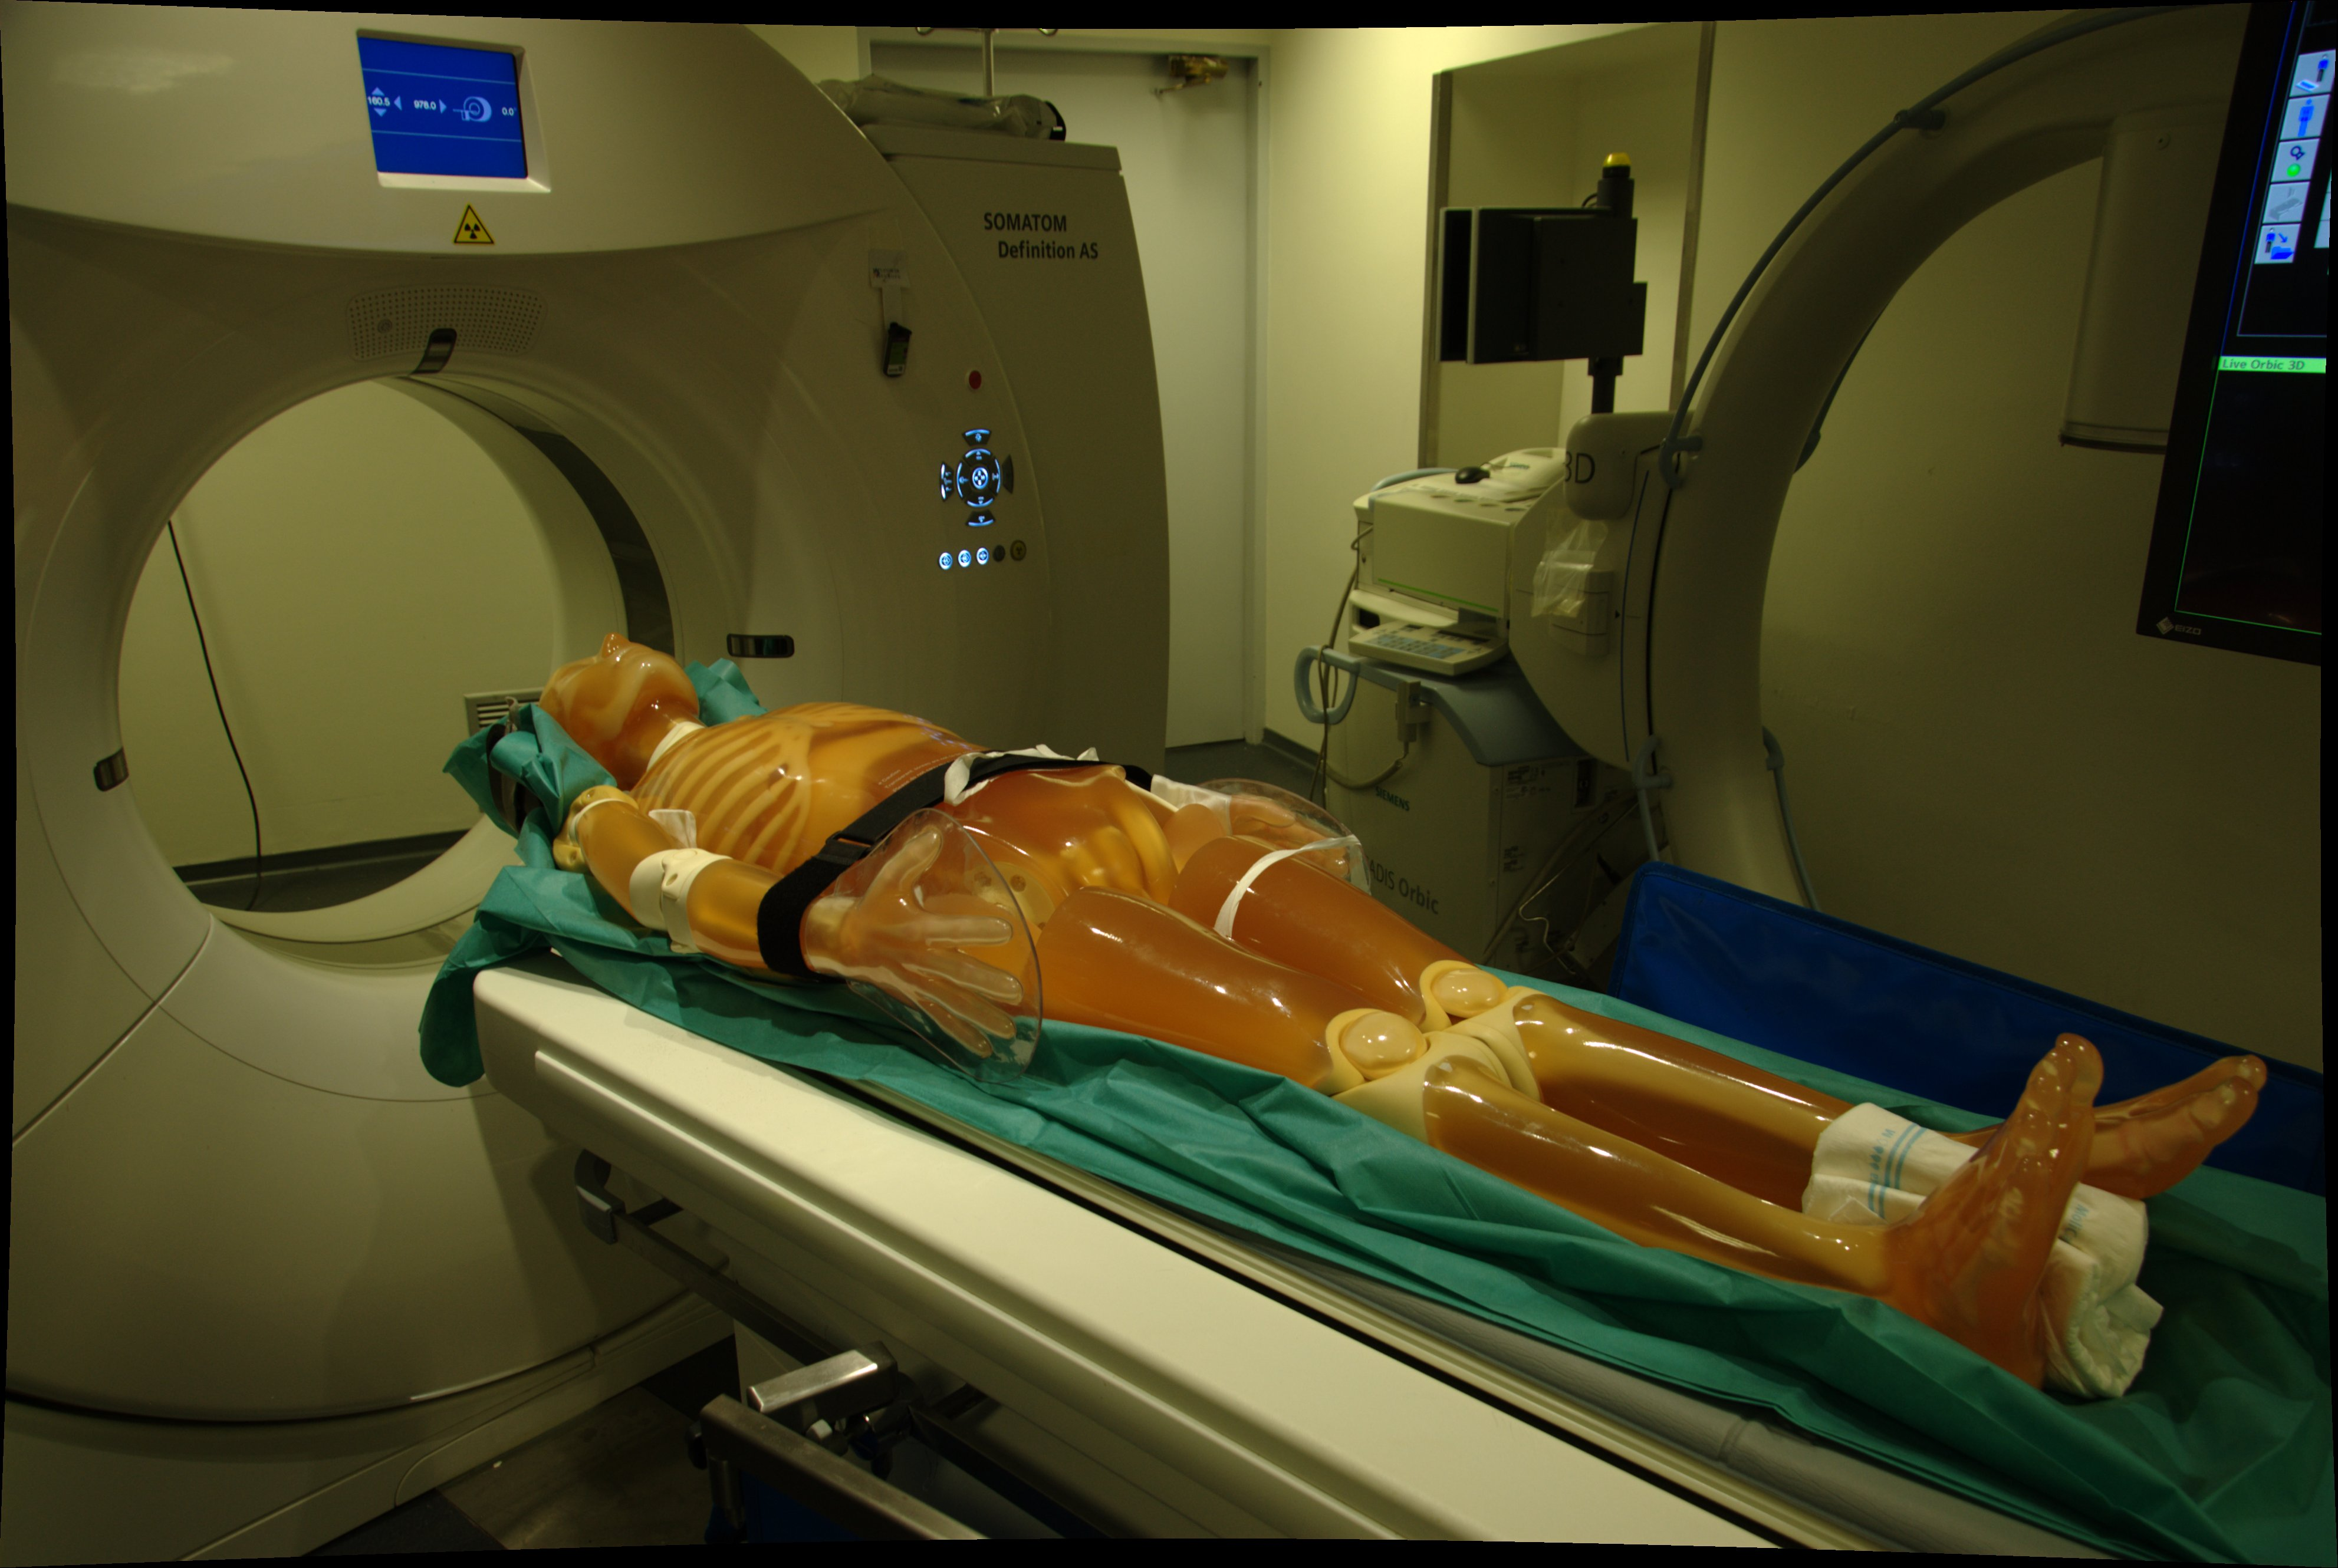
\includegraphics[width=0.6\textwidth]{../img/kyoto_irm}
\end{figure}
\vfill
Mannequin anthropomorphique scanné par rayons X à l'IRCAD.
\vfill
\end{frame}


\begin{frame}
\frametitle{Introduction}
\vfill
\begin{columns}[c]
\column{0.7\textwidth}
\begin{itemize}
\item 12 organes, grand niveau de détail géométrique ;
\item Maillage volumique de $5\,840\,122$ tétraèdres ;
\item Rapport d'échelle (vide englobant / antenne) : $1373$ ;
\item Contraintes géométriques très fortes ;
\item[=>] Utilisation de la méthode Galerkin Discontinue (GD) : solveur Teta-CLAC.
\end{itemize}
\vfill
\column{0.3\textwidth}
\begin{figure}
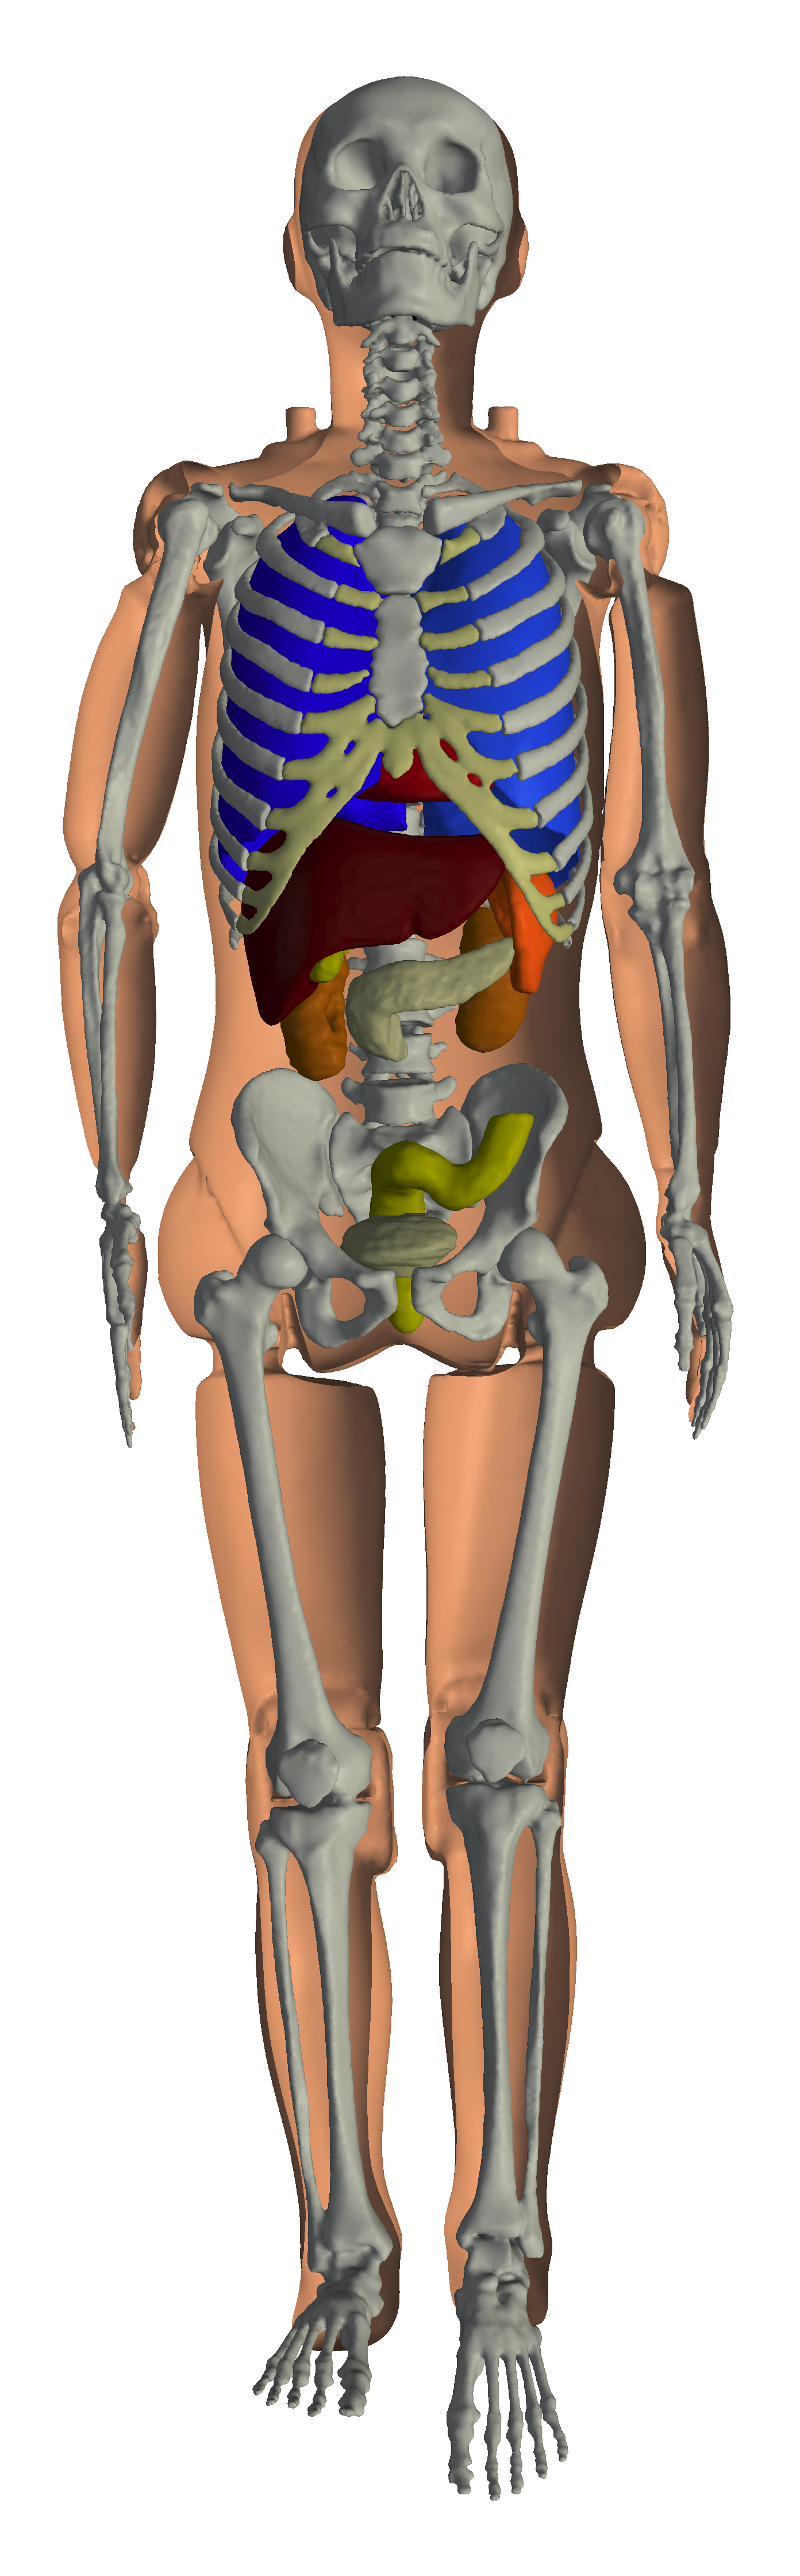
\includegraphics[width=\textwidth,trim={0 1400 0 0},clip]{../img/kyoto}
\end{figure}
\end{columns}
\vfill
\end{frame}


%----------------------------------------------------------------------------------------
%	TOC
%----------------------------------------------------------------------------------------

\begin{frame}
\frametitle{Sommaire} % Table of contents slide, comment this block out to remove it
\tableofcontents % Throughout your presentation, if you choose to use \section{} and \subsection{} commands, these will automatically be printed on this slide as an overview of your presentation
\end{frame}

%----------------------------------------------------------------------------------------
%	PRESENTATION SLIDES
%----------------------------------------------------------------------------------------

\section{Galerkin Discontinu appliqué aux équations de Maxwell}
\subsection*{Équations de Maxwell}

%\begin{frame}
\frametitle{Équations de Maxwell}
\vfill
\begin{align*}
	\Ptl{t} \EPrm \E + \ECnd \E - \Rot \H &= 0 ,
	\tag{Maxwell-Ampère}
	\\
	\Ptl{t} \HPrm \H + \HCnd \H + \Rot \E &= 0 .
	\tag{Maxwell-Faraday}
\end{align*}
\vfill
Paramètres :
\begin{itemize}
\item[]
\begin{itemize}
\item [$\E$] : champ électrique ($\in \Esp$) ;
\item [$\H$] : champ magnétique ($\in \Esp$) ;
\item [$\EPrm$] : permittivité électrique ;
\item [$\HPrm$] : perméabilité magnétique ;
\item [$\ECnd,\HCnd$] : conductivités électrique et magnétique ;
\end{itemize}
\end{itemize}
\vfill
\begin{columns}
\column{0.33\textwidth}
\begin{align*}
\Ptl{t} := \frac{\partial}{\partial t} ,
\end{align*}
\column{0.34\textwidth}
\begin{align*}
\x &= \NodeDef{\x} \in \Esp, \\
\nabla &= \Trp{(\Ptl{\x_1}, \Ptl{\x_2}, \Ptl{\x_3})} ,
\end{align*}
\column{0.33\textwidth}
\begin{align*}
\Ptl{i} := \Ptl{\x_i} .
\end{align*}
\end{columns}
\vfill
\end{frame}

 % maxwell
%\begin{frame}
\frametitle{Équations de Maxwell / Divergence}
\vfill
\begin{align*}
	\Div \EPrm \E &= 0 ,
	\tag{Maxwell-Gauss}
	\\
	\Div \HPrm \H &= 0 .
	\tag{Maxwell-Thomson}
\end{align*}
\vfill
\begin{itemize}
\item Doivent être satisfaites à l'état initial ($t = 0$) ;
\item Sont alors satisfaites au cours du temps ($t > 0$) ;
\item Inutiles dans la phase de simulation (formulation de l'algorithme).
\end{itemize}
\vfill
\end{frame}

 % divergence
\begin{frame}
\frametitle{Équations de Maxwell}
\vfill
\begin{align*}
	\Ptl{t} \EPrm \E + \ECnd \E - \Rot \H &= 0 ,
	\tag{Maxwell-Ampère}
	\\
	\Ptl{t} \HPrm \H + \HCnd \H + \Rot \E &= 0 ,
	\tag{Maxwell-Faraday}
	\\
	\Div \EPrm \E &= 0 ,
	\tag{Maxwell-Gauss}
	\\
	\Div \HPrm \H &= 0 .
	\tag{Maxwell-Thomson}
\end{align*}
\vfill
Paramètres :
\begin{itemize}
\item[]
\begin{itemize}
\item [$\E$] : champ électrique ($\in \Esp$) ;
\item [$\H$] : champ magnétique ($\in \Esp$) ;
\item [$\EPrm$] : permittivité électrique ;
\item [$\HPrm$] : perméabilité magnétique ;
\item [$\ECnd,\HCnd$] : conductivités électrique et magnétique ;
\end{itemize}
\end{itemize}
\vfill
\begin{columns}
\column{0.33\textwidth}
\begin{align*}
\Ptl{t} := \frac{\partial}{\partial t} ,
\end{align*}
\column{0.34\textwidth}
\begin{align*}
\x &= \NodeDef{\x} \in \Esp, \\
\nabla &= \Trp{(\Ptl{\x_1}, \Ptl{\x_2}, \Ptl{\x_3})} ,
\end{align*}
\column{0.33\textwidth}
\begin{align*}
\Ptl{i} := \Ptl{\x_i} .
\end{align*}
\end{columns}
\vfill
\end{frame}

 % maxwell + div
%\begin{frame}
\frametitle{Équations de Maxwell / Système de Friedrichs}
\vfill
\begin{align*}
	\Ptl{t} \EPrm \E + \ECnd \E - \Rot \H &= 0 ,
	\tag{Maxwell-Ampère}
	\\
	\Ptl{t} \HPrm \H + \HCnd \H + \Rot \E &= 0 .
	\tag{Maxwell-Faraday}
\end{align*}
\vfill
\begin{columns}%[c]
\column{.3\textwidth}
\column{.2\textwidth}
\begin{figure}
\begin{tikzpicture}[scale=0.5]
	% Fleche
	\draw[-,thick] (0,0) -- (1.4,1) -- (0.8,1) -- (0.8,3) -- (-0.8,3) -- (-0.8,1) -- (-1.4,1) -- cycle;
\end{tikzpicture}
\end{figure}
\column{.3\textwidth}
\begin{align*}
\W &= 
\begin{pmatrix}
	\E \\
	\H
\end{pmatrix}
\in \EnsR^6 ,
\\
\NC &= \dim(\EnsR^6) = 6 .
\end{align*}
\column{.2\textwidth}
\end{columns}
\vfill
\begin{align*}
	\Ptl{t} \At \W + \ACnd \W + \sum_{i=1}^3 \Aidi \W = \Src .
	\tag{Système de Friedrichs}
\end{align*}
\vfill
\begin{block}{Notation}
Dans la suite nous utilisons la convention de sommation des indices répétés,
\textit{i.e.} $\sum_{i=1}^3 \Aidi = \Aidi$.
\end{block}
\vfill
\end{frame}

 % maxwell > friedrichs
\begin{frame}
\frametitle{Équations de Maxwell / Système de Friedrichs}
\vfill
Divergence supposée nulle au cours du temps :
\begin{align*}
	\Ptl{t} \EPrm \E + \ECnd \E - \Rot \H &= 0 ,
	\tag{Maxwell-Ampère}
	\\
	\Ptl{t} \HPrm \H + \HCnd \H + \Rot \E &= 0 .
	\tag{Maxwell-Faraday}
\end{align*}
\vfill
\begin{columns}%[c]
\column{.3\textwidth}
\column{.2\textwidth}
\begin{figure}
\begin{tikzpicture}[scale=0.5]
	% Fleche
	\draw[-,thick] (0,0) -- (1.4,1) -- (0.8,1) -- (0.8,3) -- (-0.8,3) -- (-0.8,1) -- (-1.4,1) -- cycle;
\end{tikzpicture}
\end{figure}
\column{.3\textwidth}
\begin{align*}
\W &= 
\begin{pmatrix}
	\E(\x,t) \\
	\H(\x,t)
\end{pmatrix}
\in \EnsR^6 ,
\\
\NC &= \dim(\EnsR^6) = 6 .
\end{align*}
\column{.2\textwidth}
\end{columns}
\vfill
\begin{align*}
	\Ptl{t} \At \W + \ACnd \W + \sum_{i=1}^3 \Aidi \W = 0 .
	\tag{Système de Friedrichs}
\end{align*}
\vfill
\begin{itemize}
\item Matrices symétriques, $\At$ définie positive et $\ACnd$ positive ;
\item Nous considérons le problème sans sources ($\ACnd = 0$).
\end{itemize}
\begin{block}{Notation d'Einstein}
Dans la suite nous utilisons la convention de sommation des indices répétés,
\textit{i.e.} $\sum_{i=1}^3 \Aidi = \Aidi$.
\end{block}
\vfill
\end{frame}

 % maxwell > friedrichs
%\begin{frame}
\frametitle{Système de Friedrichs / Matrices}
\vfill
\scalebox{0.7}{\begin{minipage}{1.42\textwidth}
\begin{figure}
\centering
$
\begin{array}{ccc}
	\At =
	\begin{pmatrix}
		\EPrm &  &  &  &  &  \\
		 & \EPrm &  &  & 0 &  \\
		 &  & \EPrm &  &  &  \\
		 &  &  & \HPrm &  &  \\
		 & 0 &  &  & \HPrm &  \\
		 &  &  &  &  & \HPrm
	\end{pmatrix} ,
&
	\ACnd =
	\begin{pmatrix}
		\ECnd &  &  &  &  &  \\
		 & \ECnd &  &  & 0 &  \\
		 &  & \ECnd &  &  &  \\
		 &  &  & \HCnd &  &  \\
		 & 0 &  &  & \HCnd &  \\
		 &  &  &  &  & \HCnd
	\end{pmatrix} ,
&
	\Src =
	\begin{pmatrix}
		0 \\
		\vdots \\
		0
	\end{pmatrix} ,
\\
& &
\\
	\Ac{1} =
	\begin{pmatrix}
		 &  &  &  &  & 0 \\
		 & 0 &  &  & 0 & 1 \\
		 &  &  & 0 & -1 &  \\
		 &  & 0 & 0 &  &  \\
		 & 0 & -1 &  & 0 &  \\
		0 & 1 &  &  &  & 
	\end{pmatrix} ,
&
	\Ac{2} =
	\begin{pmatrix}
		 &  &  &  &  & -1 \\
		 & 0 &  &  & 0 &  \\
		 &  &  & 1 &  &  \\
		 &  & 1 &  &  &  \\
		 & 0 &  &  & 0 &  \\
		-1 &  &  &  &  & 
	\end{pmatrix} ,
&
	\Ac{3} =
	\begin{pmatrix}
		 &  &  &  & 1 & 0 \\
		 & 0 &  & -1 & 0 &  \\
		 &  & 0 & 0 &  &  \\
		 & -1 & 0 &  &  &  \\
		1 & 0 &  &  & 0 &  \\
		0 &  &  &  &  & 
	\end{pmatrix} ,
\end{array}
$
\end{figure}
\end{minipage}}
\vfill
\begin{align*}
\Aidi = 
\begin{pmatrix}
	0 & -\nabla \times \\
	\nabla \times & 0
\end{pmatrix} , \
\mathrm{avec} \
\nabla \times =
\begin{pmatrix}
	0 & -\Ptl{3} & \Ptl{2} \\
	\Ptl{3} & 0 & -\Ptl{1} \\
	-\Ptl{2} & \Ptl{1} & 0
\end{pmatrix} .
\end{align*}
\vfill
\begin{itemize}
\item Matrices symétriques ;
\item $\At$ définie positive et $\ACnd$ positive ;
\item Dans la suite nous considérons le problème sans sources ($\ACnd = 0$).
\end{itemize}
\vfill
\end{frame}

 % matrices friedrichs
\begin{frame}
\frametitle{Problème d'évolution}
\vfill
Soit $\PbEsp \in \Esp$ un ouvert et $t \in \PbTps$,
\begin{align*}
	\Ptl{t} \At \W + \Aidi \W = 0
	&\quad \mathrm{sur} \; \PbEspTps = \PbEsp \times \PbTps
	\tag{Système de Friedrichs} , \\
	\W (\x, 0) = \Winit (\x)
	&\quad \mathrm{sur} \; \PbEsp
	\tag{Condition initiale} , \\
	 \MatB \W = 0
	&\quad \mathrm{sur} \; \Bord{\PbEspTps}
	\tag{Condition limite} .
\end{align*}
\vfill
La matrice $\MatB(\x)$ dépend du type de la condition limite.
\vfill
\begin{block}{Théorème (Lax, Phillips, Rauch)}
	Si en tout point du bord :
	\begin{align*}
		\forall \W \in \ker(\MatB), \; (\Aini \W) \cdot \W \ge 0
		\tag{Unicité}
	\end{align*}
	et
	\begin{align*}
		\dim(\ker(\MatB)) = 4
		\tag{Existence} .
	\end{align*}
	alors le problème d'évolution \textbf{admet une
		unique solution}.
\end{block}
\vfill
\end{frame}

 % pb evol
\begin{frame}
\frametitle{Conditions aux limites}
\begin{columns}[c]
\column{0.5\textwidth}
\begin{align*}
	\n \times =
	\begin{pmatrix}
		0 & -\nC{3} & \nC{2} \\
		\nC{3} & 0 & -\nC{1} \\
		-\nC{2} & \nC{1} & 0
	\end{pmatrix} ,
\end{align*}
\column{0.5\textwidth}
\begin{align*}
	(\n \times)^2 = (\n \times)(\n \times) .
\end{align*}
\end{columns}
\vfill
\begin{itemize}
\item Condition de conducteur électrique parfait (PEC) :
\begin{columns}[c]
\column{0.5\textwidth}
\begin{align*}
	\n \times \E = 0 , 
\end{align*}
\column{0.5\textwidth}
\begin{align*}
	\MatB =
	\begin{pmatrix}
		a (\n \times)^2 + b \n \times & 0 \\
		c (\n \times)^2 + d \n \times & 0
	\end{pmatrix} .
\end{align*}
\end{columns}
\vfill
\item Condition d'impédance ($z$) de surface (SIBC) :
\begin{align*}
	\n \times \E + z \n \times (\n \times \H) = 0 , 
\end{align*}
\begin{align*}
	\MatB =
	\begin{pmatrix}
		a (\n \times)^2 & - a z \n \times \\
		- (1 + a z) \n \times & - (1 + a z) z (\n \times)^2
	\end{pmatrix} , \ a \le 0 .
\end{align*}
\vfill
\item Condition de Silver-Müller : SIBC avec l'impédance du vide.
\end{itemize}
\vfill
\end{frame}

 % matrices M
%\begin{frame}
\frametitle{Condition de saut}
La solution doit savoir prendre en compte les discontinuités fixes entre diélectriques : phénomène de réfraction.
\vfill
\scalebox{0.9}{\begin{minipage}{1.11\textwidth}
\begin{block}{Définition}
	Soit $\tilde{\n} = \Trp{(\Trp{\n},\nC{t})}$, avec $\n$
	un vecteur unitaire, la normale
	au support $\PbSrfTps$ d'une discontinuité spatio-temporelle de la solution du système
	de Friedrichs.
	La \textbf{relation de Rankine-Hugoniot} satisfaite sur cette discontinuité
	est donnée par l'équation :
	\begin{align*}
	\nC{t} \left( (\At)_\L \W_\L - (\At)_\R \W_\R \right) =
	\left( (\Aini)_\L \W_\L - (\Aini)_\R \W_\R \right) ,
	\end{align*}
	avec $\nC{t}$ la vitesse de propagation de la discontinuité.
\end{block}
\end{minipage}}
\vskip+1em
Application aux équations de Maxwell avec $\nC{t} = 0$ :
\begin{columns}
\column{0.5\textwidth}
\begin{align*}
\n \times (\H_\L - \H_\R) &= 0 , \\
\n \times (\E_\L - \E_\R) &= 0 .
\end{align*}
\column{0.5\textwidth}
\begin{align*}
\n \cdot (\EPrm_\L \E_\L - \EPrm_\R \E_\R) &= 0 , \\
\n \cdot (\HPrm_\L \H_\L - \HPrm_\R \H_\R) &= 0 .
\end{align*}
\end{columns}
\vfill
\begin{itemize}
\item Continuité des champs électromagnétiques tangents à $\PbSrfTps$ ;
\item Discontinuité des champs électromagnétiques normaux à $\PbSrfTps$.
\end{itemize}
\end{frame}

 % sauts
\begin{frame}
\frametitle{Condition de saut}
\vfill
\begin{itemize}
\item La solution doit savoir prendre en compte les discontinuités fixes entre diélectriques : phénomène de réfraction ;
\vfill
\item Utilisation de la relation de Rankine-Hugoniot sur la discontinuité :
\begin{align*}
	\nC{t} \left( (\At)_\L \W_\L - (\At)_\R \W_\R \right) =
	\left( (\Aini)_\L \W_\L - (\Aini)_\R \W_\R \right) \ ;
\end{align*}
\begin{itemize}
\item [$\nC{t}$] : vitesse de propagation de la discontinuité ;
\item [$\n$] : normale au support de la discontinuité ;
\end{itemize}
\vfill
\item Application aux équations de Maxwell avec $\nC{t} = 0$ (discontinuité fixe) :
\begin{columns}
\column{0.5\textwidth}
\begin{align*}
\n \times (\H_\L - \H_\R) &= 0 , \\
\n \times (\E_\L - \E_\R) &= 0 .
\end{align*}
\column{0.5\textwidth}
\begin{align*}
\n \cdot (\EPrm_\L \E_\L - \EPrm_\R \E_\R) &= 0 , \\
\n \cdot (\HPrm_\L \H_\L - \HPrm_\R \H_\R) &= 0 .
\end{align*}
\end{columns}
\vfill
\item [=>] Continuité des champs électromagnétiques tangents à la discontinuité ;
\item [=>] Discontinuité des champs électromagnétiques normaux à la discontinuité.
\end{itemize}
\vfill
\end{frame}

 % sauts

\subsection*{Formulation Galerkin Discontinue (GD)}

%\begin{frame}
\frametitle{Maillage : stratégie de zones}
\begin{columns}[c]
\column{.5\textwidth}
\begin{itemize}
\item Découpage en \textcolor{blue}{Zones}
\onslide<2->{et \textcolor{red}{Mailles} :}
\begin{align*}
\PbEsp = \textcolor{blue}{\bigcup_{k=1}^K \Adh{\PbEsp_k}}
\onslide<2->{=\textcolor{red}{\bigcup_{i=1}^\NE \Adh{\L_i}} ,}
\end{align*}
\item<3-> Maillage et interfaces :
\begin{align*}
\Mesh = &(\L_i)_{i \in \Range{1}{\NE}} , \\
\textcolor{blue}{\bigcup_{k=1}^K \Bord{\PbEsp_k}}
&\subset \textcolor{red}{\bigcup_{i=1}^\NE \Bord{\L_i}}
= \UItf ,
\end{align*}
\item<3-> Union des mailles (ouverts) :
\begin{align*}
\UElt = \bigcup_{i=1}^\NE \L_i = \PbEsp \setminus \UItf .
\end{align*}
\end{itemize}
\column{.5\textwidth}
\begin{figure}
	\begin{tikzpicture}[scale=1.5]
\onslide<1->{
\fill[gray!30] (0,0) -- (1,0.5) -- (1.5,1.2) -- (1.2,1.6) -- (1.8,2) -- (0.7,2.4) -- (-0.2,1.5) -- (-0.5,0.4) -- cycle;
}
\onslide<2->{
\draw[-,red] (1,0.5) -- (0.2,0.8);
\draw[-,red] (0,0) -- (0.2,0.8);
\draw[-,red] (-0.5,0.4) -- (0.2,0.8);
\draw[-,red] (-0.2,1.5) -- (0.2,0.8);
\draw[-,red] (-0.2,1.5) -- (1.2,1.6);
\draw[-,red] (0.7,2.4) -- (1.2,1.6);
\draw[-,red] (1.5,1.2) -- (0.2,0.8);
\draw[-,red] (1.2,1.6) -- (0.2,0.8);

\draw[-,red] (1,-0.5) -- (1,0.5);
\draw[-,red] (2,0) -- (1,0.5);
\draw[-,red] (2,0) -- (1.5,1.2);
\draw[-,red] (2.2,1) -- (1.5,1.2);
\draw[-,red] (1.8,2) -- (1.5,1.2);

\draw[red] (-0.1,0.9) node[]{$\L_1$};
\draw[red] (0.3,1.3) node[]{$\L_2$};
\draw[red] (0.5,1.8) node[]{$\L_3$};
\draw[red] (1.3,1.9) node[]{$\L_4$};
}
\onslide<1->{
\draw[-,thick,blue] (0,0) -- (1,0.5) -- (1.5,1.2) -- (1.2,1.6) -- (1.8,2);
\draw[blue] (-0.2,1.5) node[above left]{$\PbEsp_1$};
\draw[blue] (2,0) node[below right]{$\PbEsp_2$};
}
\onslide<1->{
\draw[-,thick] (0,0) -- (1,-0.5) -- (2,0) -- (2.2,1) -- (1.8,2) -- (0.7,2.4) -- (-0.2,1.5) -- (-0.5,0.4) -- cycle;
}
\onslide<1>{
\draw[arrows={latex-}] (1,1.5) -- (2,2.5) node[above right]{$\EPrm_1$};
\draw[arrows={latex-}] (1.5,0.5) -- (2.5,2.3) node[above right]{$\EPrm_2$};
}
	\end{tikzpicture}
\end{figure}
\end{columns}
\onslide<4->{
\textcolor{red}{Taille des mailles ? Fonction de la longueur d'onde : «~$\lambda_{\min} / 10$~».}
}
\end{frame}

 % maillage
\begin{frame}
\frametitle{Maillage : stratégie de zones}
\vfill
Prise en compte des discontinuités fixes dans le maillage :
\begin{columns}[c]
\column{.5\textwidth}
\begin{itemize}
\item Découpage en \textcolor{blue}{Zones}
\onslide<2->{et \textcolor{red}{Mailles} :}
\begin{align*}
\PbEsp = \textcolor{blue}{\bigcup_{k=1}^K \Adh{\PbEsp_k}}
\onslide<2->{=\textcolor{red}{\bigcup_{i=1}^\NE \Adh{\L_i}} \ ;}
\end{align*}
\item<3-> Maillage :
\begin{align*}
\Mesh = &(\L_i)_{i \in \Range{1}{\NE}} \ ;
\end{align*}
\vfill
\item<3-> Zones physiques données par le modèle CAO ;
\item<3-> Les zones permettront aussi de regrouper les mailles similaires pour appliquer des simplifications dans les calculs.
\end{itemize}
\column{.5\textwidth}
\begin{figure}
	\begin{tikzpicture}[scale=1.5]
\onslide<1->{
\fill[gray!30] (0,0) -- (1,0.5) -- (1.5,1.2) -- (1.2,1.6) -- (1.8,2) -- (0.7,2.4) -- (-0.2,1.5) -- (-0.5,0.4) -- cycle;
}
\onslide<2->{
\draw[-,red] (1,0.5) -- (0.2,0.8);
\draw[-,red] (0,0) -- (0.2,0.8);
\draw[-,red] (-0.5,0.4) -- (0.2,0.8);
\draw[-,red] (-0.2,1.5) -- (0.2,0.8);
\draw[-,red] (-0.2,1.5) -- (1.2,1.6);
\draw[-,red] (0.7,2.4) -- (1.2,1.6);
\draw[-,red] (1.5,1.2) -- (0.2,0.8);
\draw[-,red] (1.2,1.6) -- (0.2,0.8);

\draw[-,red] (1,-0.5) -- (1,0.5);
\draw[-,red] (2,0) -- (1,0.5);
\draw[-,red] (2,0) -- (1.5,1.2);
\draw[-,red] (2.2,1) -- (1.5,1.2);
\draw[-,red] (1.8,2) -- (1.5,1.2);

\draw[red] (-0.1,0.9) node[]{$\L_1$};
\draw[red] (0.3,1.3) node[]{$\L_2$};
\draw[red] (0.5,1.8) node[]{$\L_3$};
\draw[red] (1.3,1.9) node[]{$\L_4$};
}
\onslide<1->{
\draw[-,thick,blue] (0,0) -- (1,0.5) -- (1.5,1.2) -- (1.2,1.6) -- (1.8,2);
\draw[blue] (-0.2,1.5) node[above left]{$\PbEsp_1$};
\draw[blue] (2,0) node[below right]{$\PbEsp_2$};
}
\onslide<1->{
\draw[-,thick] (0,0) -- (1,-0.5) -- (2,0) -- (2.2,1) -- (1.8,2) -- (0.7,2.4) -- (-0.2,1.5) -- (-0.5,0.4) -- cycle;
}
\onslide<1>{
\draw[arrows={latex-}] (1,1.5) -- (2,2.5) node[above right]{$\EPrm_1$};
\draw[arrows={latex-}] (1.5,0.5) -- (2.5,2.3) node[above right]{$\EPrm_2$};
}
	\end{tikzpicture}
\end{figure}
\end{columns}
\vfill
\onslide<3->{
\textcolor{red}{Taille des mailles ? Fonction de la longueur d'onde : «~$\lambda_{\min} / 10$~».}
}
\end{frame}

 % maillage
\begin{frame}
\frametitle{Formulation GD / Définitions}
\vfill
Pour exprimer la formulation GD localement sur chaque maille :
\vfill
\begin{block}{Définition}
	Soit $\Mat{D} = (d_{i,j})_{i,j \in \EnsN^\star}$ une matrice réelle
	\textbf{diagonale}.\\ La \textbf{valeur absolue} de $\Mat{D}$ est définie par
	$\Abs{\Mat{D}} = (\Abs{d_{i,j}})$.
\end{block}
\vfill
\pause
\begin{block}{Définition}
	Soit $\Mat{A}$ une matrice carrée réelle et diagonalisable sur $\EnsR$. Soient
	$\Mat{P}$ une matrice inversible et $\Mat{D}$ une matrice diagonale telles que
	$\Mat{A} = \Mat{P} \Mat{D} \Inv{\Mat{P}}$.\\
	La \textbf{partie positive} de $\Mat{A}$, notée $\Pos{\Mat{A}}$, est définie par :
	\begin{align*}
		\Pos{\Mat{A}} = \frac{1}{2} \Mat{P} \left( \Mat{D} + \Abs{\Mat{D}} \right) \Inv{\Mat{P}} .
	\end{align*}
	La \textbf{partie négative} de $\Mat{A}$, notée $\Neg{\Mat{A}}$, est définie par :
	\begin{align*}
		\Neg{\Mat{A}} = \frac{1}{2} \Mat{P} \left( \Mat{D} - \Abs{\Mat{D}} \right) \Inv{\Mat{P}} .
	\end{align*}
\end{block}
\vfill
\end{frame}

 % definitions A+ et A-
\begin{frame}
\frametitle{Formulation GD / Construction}
\vfill
Étapes de construction de la formulation GD :
\scalebox{0.8}{\begin{minipage}{1.25\textwidth}
\begin{enumerate}[(i)]
\item \textbf{Formulation faible} (fonction test) du problème d'évolution avec \textbf{conditions aux limites} ;
\item Prise en compte des \textbf{discontinuités} de la solution en appliquant la \textbf{condition de saut} ;
\item \textbf{Formulation locale} aux mailles (fonction test nulle en-dehors) ;
\item \textbf{Intégration par parties} (Green) afin de transférer la dérivation spatiale sur la fonction test.
\end{enumerate}
\end{minipage}}
%\vfill
\vskip+1em
\begin{columns}%[c]
\column{0.7\textwidth}
Nous obtenons alors la formulation GD du problème :
\scalebox{0.9}{\begin{minipage}{1.11\textwidth}
\begin{align*}
	\mathcal{H} &= \lbrace
		f \in \mathrm{L}^2(\PbEsp) :
		\forall \L \in \Mesh,
		f_{\vert \L} \in \mathcal{C}^1(\Adh{\L})
	\rbrace , \\
	\W &\in \mathcal{C}^1(\PbTps,\mathcal{H}^\NC) :
	\forall \L \in \Mesh, \forall \psi \in \mathcal{C}^1(\Adh{\L}), \\
	0 &= \int_{\L} \Ptl{t} \At \W \psi d\x
	- \int_{\L} \Aidi \psi \W d\x
	+ \int_{\Bord{\L} \cap \Bord{\PbEsp}}
		(\Aini + \MatB) \W \psi ds \\
	&+ \int_{\Bord{\L} \setminus \Bord{\PbEsp}}
		(\Pos{\Aini} \W_\L + \Neg{\Aini} \W_\R) \psi ds .
\end{align*}
\end{minipage}}
\column{0.3\textwidth}
\begin{figure}
	\begin{tikzpicture}[scale=0.6]
		\draw [arrows={-latex},thick,red] (2,2.6)
			-- node[red, midway, below] {\small$\n$} (2.7,2.6); % normal
		\draw [thick] (0.7,1) -- node[midway, right] {\small$\L$} (0.4,3.7)
			-- (2,3.2) -- (2,1.7) -- cycle; % polygon L
		\draw [thick] (2,1.7) -- (2,3.2) -- (3.6,3)
			-- node[midway, left] {\small$\R$} (3.3,1) -- cycle; % polygon R
		\draw [arrows={-latex},red] (1,4) node[above,red] {\small$\Bord{\L} \cap \Bord{\R}$}
			-- (2,2.9); % flèche interface
		\draw (0.7,1) -- (0.2,0.5); % arêtes sortantes
		\draw (0.4,3.7) -- (0,3.8);
		\draw (2,3.2) -- (2.1,3.8);
		\draw (3.6,3) -- (4.1,3.1);
		\draw (3.3,1) -- (3.7,0.7);
		\draw (2,1.7) -- (1.9,1.1);
	\end{tikzpicture}
\end{figure}
\end{columns}
\vfill
\begin{block}{Théorème}
	La méthode est stable si en tout point du bord
	la matrice $\frac{1}{2} \Aini + \MatB$ est positive.
\end{block}
\vfill
\end{frame}

 % formulation
\begin{frame}
\frametitle{Formulation GD / Flux numérique}
\vfill
Nous introduisons alors le flux numérique :
\begin{align}
	\Flux{\W_\L}{\W_\R}{\n} = \Pos{\Aini} \W_\L + \Neg{\Aini} \W_\R
	\tag{Flux numérique}
\end{align}
et le flux de bord :
\begin{align}
	\FluxB{\W}{\n} = (\Aini + \MatB) \W .
	\tag{Flux de bord}
\end{align}
\vfill
\begin{block}{Propriétés}
Le flux numérique vérifie :
\begin{subequations}
\begin{align*}
	\Flux{\W}{\W}{\n} &= \Aini \W ,
	\tag{Consistance} \\
	\Flux{\W_\L}{\W_\R}{-\n} &= - \Flux{\W_\R}{\W_\L}{\n} .
	\tag{Conservation}
\end{align*}
\end{subequations}
\end{block}
\vfill
Autres choix possibles :
\begin{align*}
	\F_\alpha =
	\begin{pmatrix}
		- \frac{1}{2} \n \times (\H_\L + \H_\R)
		+ \alpha (\n \times)^2 (\E_\R - \E_\L) \\
		\frac{1}{2} \n \times (\E_\L + \E_\R)
		+ \alpha (\n \times)^2 (\H_\R - \H_\L)
	\end{pmatrix} .
\end{align*}
\vfill
\end{frame}

 % flux

\begin{frame}
\frametitle{Maxwell - GD / Conclusion}
\vfill
Nous avons vu :
\begin{itemize}
\item Rappel des équations de Maxwell (Friedrichs) ;
\item Étude du problème d'évolution : conditions aux limites et de saut ;
\item Stratégie de découpage en zones homogènes (zones, mailles) ;
\item Formulation GD : évaluation locale (aux mailles) de la \textbf{dérivée temporelle}.
\end{itemize}
\vfill
\pause
Nous allons voir :
\begin{itemize}
\item Passage du problème continu à la résolution discrète (dimension finie);
\item Simplifications induites par le choix de l'espace d'approximation ;
\item Améliorations algorithmiques apportées.
\end{itemize}
\vfill
\end{frame}




\section{Optimisations}

\subsection{Espace d'approximation et simplifications}

\begin{frame}
\frametitle{Espace d'approximation / Élément de référence}
\vfill
\begin{columns}[c]
\column{.5\textwidth}
\begin{itemize}
\item Choix des hexaèdres ;
\item Cube unité, noté $\HexaRef = \ItvCC{0}{1}^{3}$ ;
\item Faces notées $(\QuadRef_f)_{f \in \Range{0}{5}}$ ;
\item Permet de se ramener à un espace identique pour chaque maille ;
\item Passage des tétraèdres aux hexaèdres :
\end{itemize}
\vfill
\begin{figure}
\centering
		\begin{tikzpicture}[scale=3,rotate around x=270,rotate around z=45]
		%\draw[very thick] (0,0,0) -- (1,0,0) -- (0.5,0.5,0.7) -- (0,1,0) -- cycle;
		%\draw[very thick] (0,0,0) -- (0.5,0.5,0.7);
		%\draw[dashed,very thick] (1,0,0) -- (0,1,0);
		
		\fill[green!20,opacity=0.5] (0,1,0) -- (0,0.5,0) -- (0.3333,0.3333,0) -- (0.5,0.5,0) -- (0.5,0.5,0.2333) -- (0.25,0.75,0.35) -- cycle;
		
		\fill[blue!20,opacity=0.5] (1,0,0) -- (0.5,0,0) -- (0.3333,0.3333,0) -- (0.375,0.375,0.175) -- (0.5,0.5,0.2333) -- (0.75,0.25,0.35) -- cycle;
		
		\fill[yellow!20,opacity=0.5] (0.5,0.5,0.7) -- (0.75,0.25,0.35) -- (0.5,0.1666,0.2333) -- (0.375,0.375,0.175) -- (0.1666,0.5,0.2333) -- (0.25,0.75,0.35) -- cycle;

		\fill[red!20,opacity=0.5] (0,0,0) -- (0,0.5,0) -- (0.1666,0.5,0.2333) -- (0.25,0.25,0.35) -- (0.5,0.1666,0.2333) -- (0.5,0,0) -- cycle;
		
		\draw[green,dashed,very thick] (0,1,0) -- (0.5,0.5,0);
		\draw[green,dashed] (0.5,0.5,0) -- (0.3333,0.3333,0);
		\draw[green,dashed] (0.3333,0.3333,0) -- (0,0.5,0);
		\draw[green,very thick] (0,0.5,0) -- (0,1,0);
		\draw[green,dashed] (0.25,0.75,0.35) -- (0.5,0.5,0.2333);
		\draw[green,dashed] (0.5,0.5,0.2333) -- (0.375,0.375,0.175);
		\draw[green,dashed] (0.375,0.375,0.175) -- (0.1666,0.5,0.2333);
		\draw[green] (0.1666,0.5,0.2333) -- (0.25,0.75,0.35);
		\draw[green,very thick] (0,1,0) -- (0.25,0.75,0.35);
		\draw[green,dashed] (0.5,0.5,0) -- (0.5,0.5,0.2333);
		\draw[green,dashed] (0.3333,0.3333,0) -- (0.375,0.375,0.175);
		\draw[green] (0,0.5,0) -- (0.1666,0.5,0.2333);
		
		\draw[blue,very thick] (1,0,0) -- (0.5,0,0);
		\draw[blue,dashed] (0.5,0,0) -- (0.3333,0.3333,0);
		\draw[blue,dashed] (0.3333,0.3333,0) -- (0.5,0.5,0);
		\draw[blue,dashed,very thick] (0.5,0.5,0) -- (1,0,0);
		\draw[blue] (0.75,0.25,0.35) -- (0.5,0.1666,0.2333);
		\draw[blue,dashed] (0.5,0.1666,0.2333) -- (0.375,0.375,0.175);
		\draw[blue,dashed] (0.375,0.375,0.175) -- (0.5,0.5,0.2333);
		\draw[blue,dashed] (0.5,0.5,0.2333) -- (0.75,0.25,0.35);
		\draw[blue,very thick] (1,0,0) -- (0.75,0.25,0.35);
		\draw[blue] (0.5,0,0) -- (0.5,0.1666,0.2333);
		\draw[blue,dashed] (0.3333,0.3333,0) -- (0.375,0.375,0.175);
		\draw[blue,dashed] (0.5,0.5,0) -- (0.5,0.5,0.2333);
		
		\draw[yellow,very thick] (0.5,0.5,0.7) -- (0.25,0.25,0.35);
		\draw[yellow] (0.25,0.25,0.35) -- (0.5,0.1666,0.2333);
		\draw[yellow] (0.5,0.1666,0.2333) -- (0.75,0.25,0.35);
		\draw[yellow,very thick] (0.75,0.25,0.35) -- (0.5,0.5,0.7);
		\draw[yellow] (0.25,0.75,0.35) -- (0.1666,0.5,0.2333);
		\draw[yellow,dashed] (0.1666,0.5,0.2333) -- (0.375,0.375,0.175);
		\draw[yellow,dashed] (0.375,0.375,0.175) -- (0.5,0.5,0.2333);
		\draw[yellow,dashed] (0.5,0.5,0.2333) -- (0.25,0.75,0.35);
		\draw[yellow,very thick] (0.5,0.5,0.7) -- (0.25,0.75,0.35);
		\draw[yellow] (0.25,0.25,0.35) -- (0.1666,0.5,0.2333);
		\draw[yellow,dashed] (0.5,0.1666,0.2333) -- (0.375,0.375,0.175);
		\draw[yellow,dashed] (0.75,0.25,0.35) -- (0.5,0.5,0.2333);

		\draw[red,very thick] (0,0,0) -- (0,0.5,0);
		\draw[red,dashed] (0,0.5,0) -- (0.3333,0.3333,0);
		\draw[red,dashed] (0.3333,0.3333,0) -- (0.5,0,0);
		\draw[red,very thick] (0.5,0,0) -- (0,0,0);
		\draw[red] (0.25,0.25,0.35) -- (0.1666,0.5,0.2333);
		\draw[red,dashed] (0.1666,0.5,0.2333) -- (0.375,0.375,0.175);
		\draw[red,dashed] (0.375,0.375,0.175) -- (0.5,0.1666,0.2333);
		\draw[red] (0.5,0.1666,0.2333) -- (0.25,0.25,0.35);
		\draw[red,very thick] (0,0,0) -- (0.25,0.25,0.35);
		\draw[red] (0,0.5,0) -- (0.1666,0.5,0.2333);
		\draw[red,dashed] (0.3333,0.3333,0) -- (0.375,0.375,0.175);
		\draw[red] (0.5,0,0) -- (0.5,0.1666,0.2333);
		
		% centre : (0.375,0.375,0.175)
		% face 1 : (0.3333,0.3333,0)
		% face 2 : (0.5,0.1666,0.2333)
		% face 3 : (0.5,0.5,0.2333)
		% face 4 : (0.1666,0.5,0.2333)
		% edge 1 : (0.5,0,0)
		% edge 2 : (0.5,0.5,0)
		% edge 3 : (0,0.5,0)
		% edge 4 : (0.25,0.25,0.35)
		% edge 5 : (0.75,0.25,0.35)
		% edge 6 : (0.25,0.75,0.35)
		
		
		
		%\draw[very thick] (0,0,0) -- (1,0,0) -- (0,1,0) -- cycle;
		%\draw[blue] (0,0,0) -- (0.5,0.5,0.7);
		%\draw[red] (1,0,0) -- (0.5,0.5,0.7);
		%\draw[green] (0,1,0) -- (0.5,0.5,0.7);
		\end{tikzpicture}
\end{figure}
\column{.5\textwidth}
\begin{figure}
\centering
\begin{tikzpicture}[scale=3,rotate around x=270,rotate around z=258]
	% cube arriere
	\draw [dashed] (0,0,0) -- (1,0,0);
	\draw [dashed] (0,0,0) -- (0,1,0);
	\draw [dashed] (0,0,0) -- (0,0,1);

	% cube avant
	\draw [-] (1,1,0) -- (1,0,0);
	\draw [-] (0,1,1) -- (0,1,0);
	\draw [-] (1,0,1) -- (0,0,1);

	\draw [-] (1,1,0) -- (0,1,0);
	\draw [-] (0,1,1) -- (0,0,1);
	\draw [-] (1,0,1) -- (1,0,0);

	\draw [-] (1,1,0) -- (1,1,1);
	\draw [-] (0,1,1) -- (1,1,1);
	\draw [-] (1,0,1) -- (1,1,1);
\end{tikzpicture}
\end{figure}
\end{columns}
\vfill
\end{frame}

 % cube
\begin{frame}
\frametitle{Espace d'approximation / Points de volume}
\vfill
\begin{columns}[c]
\column{.5\textwidth}
\begin{itemize}
\item Ordre d'interpolation $\Deg \in \EnsN^\star$ ;
\item $(\Deg + 1)^3$ points et poids d'intégration de Gauss-Legendre :
\begin{align*}
&(\GLN{i})_{i \ge 0} \subset \HexaRef , \\
&(\GLW{i})_{i \ge 0} \subset \EnsR^{\star +} \ ;
\end{align*}
\item Formule de quadrature volumique :
\begin{align*}
\int_{\HexaRef} \psi (\xref) d\xref \approx
	\sum_{i} \GLW{i} \psi (\GLN{i}) .
\end{align*}
\end{itemize}
\column{.5\textwidth}
\begin{figure}
\centering
\begin{tikzpicture}[scale=3,rotate around x=270,rotate around z=258]
	% cube arriere
	\draw [dashed] (0,0,0) -- (1,0,0);
	\draw [dashed] (0,0,0) -- (0,1,0);
	\draw [dashed] (0,0,0) -- (0,0,1);

	\draw (0.7,1.25) node {\small$d=2$};

	% gauss legendre: 0.1127, 0.5, 0.8873
	\def \pgs {0.1127,0.5,0.8873}

	% points volumiques
	\foreach \x in \pgs {
	\foreach \y in \pgs {
	\foreach \z in \pgs {
		\draw (\x,\y,\z) node[blue] {$\bm{+}$};
	}}}
	% lignes pointilées direction x
	\foreach \y in \pgs
	\foreach \z in \pgs {
		\draw [dotted] (0,\y,\z) -- (1,\y,\z);
	}
	% lignes pointilées direction y
	\foreach \x in \pgs
	\foreach \z in \pgs {
		\draw [dotted] (\x,0,\z) -- (\x,1,\z);
	}
	% lignes pointilées direction z
	\foreach \x in \pgs
	\foreach \y in \pgs {
		\draw [dotted] (\x,\y,0) -- (\x,\y,1);
	}

	% cube avant
	\draw [-] (1,1,0) -- (1,0,0);
	\draw [-] (0,1,1) -- (0,1,0);
	\draw [-] (1,0,1) -- (0,0,1);

	\draw [-] (1,1,0) -- (0,1,0);
	\draw [-] (0,1,1) -- (0,0,1);
	\draw [-] (1,0,1) -- (1,0,0);

	\draw [-] (1,1,0) -- (1,1,1);
	\draw [-] (0,1,1) -- (1,1,1);
	\draw [-] (1,0,1) -- (1,1,1);
\end{tikzpicture}
\end{figure}
\end{columns}
\vfill
\end{frame}

 % pt volume
\begin{frame}
\frametitle{Espace d'approximation / Points de faces}
\vfill
\begin{columns}[c]
\column{.5\textwidth}
\begin{itemize}
\item $(\Deg + 1)^2$ points et poids d'intégration de Gauss-Legendre par face :
\begin{align*}
&(\GLN{f,i})_{i \ge 0} \subset \QuadRef_f , \\
&(\GLW{f,i})_{i \ge 0} \subset \EnsR^{\star +} \ ;
\end{align*}
\item Projetés orthogonaux sur les faces des points volumiques : $i = \pi(f,j)$ ;
\item Formule de quadrature surfacique :
\begin{align*}
\int_{\QuadRef_f} \psi (\xref) d\xref \approx
	\sum_{i} \GLW{f,i} \psi (\GLN{f,i}) .
\end{align*}
\end{itemize}
\column{.5\textwidth}
\begin{figure}
\centering
\begin{tikzpicture}[scale=3,rotate around x=270,rotate around z=258]
	% cube arriere
	\draw [dashed] (0,0,0) -- (1,0,0);
	\draw [dashed] (0,0,0) -- (0,1,0);
	\draw [dashed] (0,0,0) -- (0,0,1);

	\draw (0.7,1.25) node {\small$d=2$};
\onslide<2>{
	\draw (0.3,-0.25,1) node {\textcolor{red}{\small$f=5$}};
}

	% gauss legendre: 0.1127, 0.5, 0.8873
	\def \pgs {0.1127,0.5,0.8873}
	\def \c {0,1}

	% points surface et lignes pointilées direction x
	\foreach \y in \pgs
	\foreach \z in \pgs {
		\draw [dotted] (0,\y,\z) -- (1,\y,\z);
		\foreach \x in \c {
			\draw (\x,\y,\z) node[green] {$\bm{\times}$};
		}
	}
	% points surface et lignes pointilées direction y
	\foreach \x in \pgs
	\foreach \z in \pgs {
		\draw [dotted] (\x,0,\z) -- (\x,1,\z);
		\foreach \y in \c {
			\draw (\x,\y,\z) node[green] {$\bm{\times}$};
		}
	}
	% points surface et lignes pointilées direction z
	\foreach \x in \pgs
	\foreach \y in \pgs {
		\draw [dotted] (\x,\y,0) -- (\x,\y,1);
		\draw (\x,\y,0) node[green] {$\bm{\times}$};
\onslide<1>{
		\draw (\x,\y,1) node[green] {$\bm{\times}$};
}
\onslide<2>{
		\draw (\x,\y,1) node[red] {$\bm{\times}$};
}
	}

	% cube avant
	\draw [-] (1,1,0) -- (1,0,0);
	\draw [-] (0,1,1) -- (0,1,0);
	\draw [-] (1,0,1) -- (0,0,1);

	\draw [-] (1,1,0) -- (0,1,0);
	\draw [-] (0,1,1) -- (0,0,1);
	\draw [-] (1,0,1) -- (1,0,0);

	\draw [-] (1,1,0) -- (1,1,1);
	\draw [-] (0,1,1) -- (1,1,1);
	\draw [-] (1,0,1) -- (1,1,1);
\end{tikzpicture}
\end{figure}
\end{columns}
\vfill
\end{frame}

 % pt face
\begin{frame}
\frametitle{Espace d'approximation / Fonctions de base}
\vfill
\begin{itemize}
\item Polynômes de Lagrange $(l_p)_{p \in \RangeDeg}$
associés aux points de Gauss-Legendre $(\GLn_p)_{p \in \RangeDeg}$ en dimension 1 :
\begin{columns}[c]
\column{.5\textwidth}
\begin{align*}
	l_p(\GLn) = \prod_{\substack{q=0 \\ q \ne p}}^{\Deg}
	\frac{\GLn - \GLn_q}{\GLn_p - \GLn_q} ,
\end{align*}
\column{.5\textwidth}
\begin{align*}
l_p(\GLn_q) = \delta_{p,q} \ ;
\end{align*}
\end{columns}
\item Produits tensoriels des polynômes $(l_p)$ en dimension 3 :
\begin{align*}
	\PsiRef{i} : \HexaRef &\to \EnsR
	\tag{Base approx.} \\
	\xref &\mapsto
	l_p(\xref_1)
	l_q(\xref_2)
	l_r(\xref_3) , \\
	i &= p + (\Deg + 1)(q + (\Deg + 1) r) \ ;
\end{align*}
\item Vérifient, par définition (numérotation identique aux points) :
\begin{enumerate}[(i)]
\item Volume : $\PsiRef{i}(\GLN{j}) = \delta_{i,j}$ ;
\item Faces : $\PsiRef{i}(\GLN{f,j})
	\begin{cases}
	\ne 0 & \mathrm{si} \ \pi(f,i) = j , \\ 
	= 0 & \mathrm{sinon} .
	\end{cases}$\\
	\textit{i.e.} non nulle uniquement sur les projetés orthogonaux.
\end{enumerate}
\end{itemize}
\vfill
\end{frame}

 % base ref
\begin{frame}
\frametitle{Espace d'approximation / Fonctions de base physiques}
\vfill
\begin{itemize}
\item Transformation géométrique de $\HexaRef$ vers une maille $\L$ :
\begin{align*}
	\TGeo{\L} : \HexaRef &\to \L \\
	\xref &\mapsto \x \ ;
\end{align*}
\vfill
\item Transformation devant être bijective (inverse calculé par la méthode de Newton) :
\begin{align*}
	\Jac{\TGeo{\L}} = \Det{\TGeo{\L}'} > 0 \ ;
\end{align*}
\vfill
\item Fonctions de base dans la maille physique :
\begin{align*}
	\forall \xref \in \HexaRef, \
	\PsiPhy{\L}{i} \circ \TGeo{\L}(\xref) =
	\PsiRef{i}(\xref) ,
\end{align*}
\begin{align*}
	\PsiPhy{\L}{i}(\x) =
	\begin{cases}
		\PsiRef{i} \circ \Inv{\TGeo{\L}}(\x) & \x \in \L , \\
		0 & \x \notin \L .
	\end{cases}
\end{align*}
\end{itemize}
\vfill
\end{frame}

 % base phy (trans. geo)
\begin{frame}
\frametitle{Problème semi-discret}
\vfill
Décomposition des champs électromagnétiques dans la base d'approximation :
\begin{align*}
	\W(\x,t) \approx \Wd(\x,t) &= \sum_{\L \in \Mesh} \sum_{i}
		\Wd_{\L,i}(t) \PsiPhy{\L}{i}(\x) ,
	\\
	\Ptl{t}\W(\x,t) \approx \Ptl{t}\Wd(\x,t) &= \sum_{\L \in \Mesh} \sum_{i}
		\Wd'_{\L,i}(t) \PsiPhy{\L}{i}(\x) ,
\end{align*}
avec $\Wd$ la solution du problème dit « semi-discret ».
\vfill
\begin{itemize}
\item Les seules valeurs aux points d'interpolation volumiques suffisent à définir la solution semi-discrète.
\item La solution du problème semi-discret $\Wd$
converge vers la solution du problème continu $\W$
lorsque le \textit{pas de maillage} tend vers zéro (théorème : Lesaint, Johnson).
\end{itemize}
\vfill
Pourquoi les hexaèdres ? Le choix de cet espace d'approximation implique des simplifications.
\vfill
\end{frame}
\renewcommand{\W}{\Vec{\mathrm{w}}} % Solution discrète dans la suite

 % pb semi discret

\subsection*{Simplifications}

\begin{frame}
\frametitle{Simplifications / Terme de masse}
\vfill
Pour une fonction de base $\PsiPhy{\L}{i}$ fixée :
\begin{align*}
	\int_{\L} \Ptl{t} \At \W \PsiPhy{\L}{i} d\x
	&\approx \int_{\L} \sum_{j}
		\At \W'_{\L,j} \PsiPhy{\L}{j} \PsiPhy{\L}{i} d\x
		\tag{Base} \\
	&= \int_{\HexaRef} \sum_{j}
		\At \W'_{\L,j}
		\PsiRef{j} \PsiRef{i}
		\Jac{\TGeo{\L}} d\xref
		\tag{Chgt. var.} \\
	&\approx \sum_{k} \sum_{j}
		\GLW{k} \At \W'_{\L,j}
		\PsiRef{j}(\GLN{k}) \PsiRef{i}(\GLN{k})
		\Jac{\TGeo{\L}}(\GLN{k})
		\tag{Quadrature} \\
	&= \GLW{i} \At \W'_{\L,i}
		\Jac{\TGeo{\L}} (\GLN{i})
		\tag{Termes nuls} .
\end{align*}
\vfill
\begin{itemize}
\item Le terme de masse fait intervenir une matrice diagonale.
\end{itemize}
\end{frame}

 % masse
\begin{frame}
\frametitle{Simplifications / Terme de rigidité (volume)}
\vfill
Pour une fonction de base $\PsiPhy{\L}{i}$ fixée :
\scalebox{0.9}{\begin{minipage}{1.11\textwidth}
\begin{align*}
	\int_{\L} &\Flux{\W}{\W}{\nabla \PsiPhy{\L}{i}} d\x \\
	&= \int_{\HexaRef}
		\Flux{\W \circ \TGeo{\L}}{\W \circ \TGeo{\L}}{\nabla \PsiPhy{\L}{i} \circ \TGeo{\L}}
		\Jac{\TGeo{\L}} d\xref
		\tag{Chgt. var.} \\
	&\approx \int_{\HexaRef}
		\Flux{\sum_{k}
		\W_{\L,k} \PsiRef{k}}{\sum_{k}
		\W_{\L,k} \PsiRef{k}}{\Com{\TGeo{\L}'} \hat{\nabla} \PsiRef{i}}
		d\xref
		\tag{Base} \\
	&\approx \sum_{j} \GLW{j}
		\Flux{\sum_{k}
		\W_{\L,k} \PsiRef{k}(\GLN{j})}{\sum_{k}
		\W_{\L,k} \PsiRef{k}(\GLN{j})}{\Com{\TGeo{\L}'} \hat{\nabla} \PsiRef{i}(\GLN{j})}
		\tag{Quadrature} \\
	&= \sum_{j} \GLW{j}
		\Flux{\W_{\L,j}}{\W_{\L,j}}{\Com{\TGeo{\L}'} \hat{\nabla} \PsiRef{i}(\GLN{j})}
		\tag{Termes nuls} .
\end{align*}
\end{minipage}}
\vfill
\begin{itemize}
\item Changement de variable : linéarité du flux et $\Com{\TGeo{\L}'} \TGeo{\L}' = \det (\TGeo{\L}') \Mat{I}$ ;
\item Flux : évaluation du gradient de la fonction de base sur tous les points de volume ;
\item Des simplifications apparaissent sur le gradient de la fonction de base.
\end{itemize}
\vfill
\end{frame}

 % volume
\begin{frame}
\frametitle{Simplifications / Terme de rigidité / Gradient}
\vfill
\begin{columns}%[c]
\column{.5\textwidth}
\begin{itemize}
\item Pour une fonction de base $\PsiRef{i}$ donnée, la valeur de son gradient
en un point d'intégration $\GLN{j}$ est non nulle uniquement si ce point est aligné dans une direction avec le point
$\GLN{i}$ associé à la fonction ;
\item<5-> Seule la composante correspondant à la direction d'alignement est non nulle ;
\end{itemize}
\column{.5\textwidth}
\begin{figure}
\centering
\begin{tikzpicture}[scale=3,rotate around x=270,rotate around z=258]
	% cube
	\draw [dashed] (0,0,0) -- (1,0,0);
	\draw [dashed] (0,0,0) -- (0,1,0);
	\draw [dashed] (0,0,0) -- (0,0,1);

	\draw [-] (1,1,0) -- (1,0,0);
	\draw [-] (0,1,1) -- (0,1,0);
	\draw [-] (1,0,1) -- (0,0,1);

	\draw [-] (1,1,0) -- (0,1,0);
	\draw [-] (0,1,1) -- (0,0,1);
	\draw [-] (1,0,1) -- (1,0,0);

	\draw [-] (1,1,0) -- (1,1,1);
	\draw [-] (0,1,1) -- (1,1,1);
	\draw [-] (1,0,1) -- (1,1,1);
	
	\draw (0.7,1.25) node {\small$d=3$};

\onslide<1>{
	% gauss legendre: 0.06943, 0.33, 0.67, 0.9306
	\def \rpg {0.67}
	\def \pgs {0.06943,0.33,0.9306}
	% points volumiques
	\foreach \x in \pgs {
	\foreach \y in \pgs {
	\foreach \z in \pgs {
		\draw (\x,\y,\z) node[blue] {$\bm{+}$};
	}}}
	\foreach \y in \pgs {
	\foreach \z in \pgs {
		\draw (\rpg,\y,\z) node[blue] {$\bm{+}$};
	}}
	\foreach \x in \pgs {
	\foreach \z in \pgs {
		\draw (\x,\rpg,\z) node[blue] {$\bm{+}$};
	}}
	\foreach \x in \pgs {
	\foreach \y in \pgs {
		\draw (\x,\y,\rpg) node[blue] {$\bm{+}$};
	}}
	% points volumiques alignés
	\foreach \x in \pgs {
		\draw (\x,\rpg,\rpg) node[blue] {$\bm{+}$};
		\draw (\rpg,\x,\rpg) node[blue] {$\bm{+}$};
		\draw (\rpg,\rpg,\x) node[blue] {$\bm{+}$};
	}
	% point volumique de référence
	\draw (\rpg,\rpg,\rpg) node[red] {$\bm{\times}$};

	\def \apgs {0.06943,0.33,0.67,0.9306}
	% points surface et lignes pointilées direction x
	\foreach \y in \apgs
	\foreach \z in \apgs {
		\draw [dotted] (0,\y,\z) -- (1,\y,\z);
%		\foreach \x in \c {
%			\draw (\x,\y,\z) node[green] {$\bm{\times}$};
%		}
	}
	% points surface et lignes pointilées direction y
	\foreach \x in \apgs
	\foreach \z in \apgs {
		\draw [dotted] (\x,0,\z) -- (\x,1,\z);
%		\foreach \y in \c {
%			\draw (\x,\y,\z) node[green] {$\bm{\times}$};
%		}
	}
	% points surface et lignes pointilées direction z
	\foreach \x in \apgs
	\foreach \y in \apgs {
		\draw [dotted] (\x,\y,0) -- (\x,\y,1);
%		\foreach \z in \c {
%			\draw (\x,\y,\z) node[green] {$\bm{\times}$};
%		}
	}
}
\onslide<2>{
	% gauss legendre: 0.06943, 0.33, 0.67, 0.9306
	\def \rpg {0.67}
	\def \pgs {0.06943,0.33,0.9306}
	% pointillés
	\draw [dotted] (0,\rpg,\rpg) -- (1,\rpg,\rpg);
	% points volumiques alignés
	\foreach \x in \pgs {
		\draw (\x,\rpg,\rpg) node[blue] {$\bm{+}$};
	}
	% point volumique de référence
	\draw (\rpg,\rpg,\rpg) node[red] {$\bm{\times}$};
}
\onslide<3>{
	% gauss legendre: 0.06943, 0.33, 0.67, 0.9306
	\def \rpg {0.67}
	\def \pgs {0.06943,0.33,0.9306}
	% pointillés
	\draw [dotted] (0,\rpg,\rpg) -- (1,\rpg,\rpg);
	\draw [dotted] (\rpg,0,\rpg) -- (\rpg,1,\rpg);
	% points volumiques alignés
	\foreach \x in \pgs {
		\draw (\x,\rpg,\rpg) node[blue] {$\bm{+}$};
		\draw (\rpg,\x,\rpg) node[blue] {$\bm{+}$};
	}
	% point volumique de référence
	\draw (\rpg,\rpg,\rpg) node[red] {$\bm{\times}$};
}
\onslide<4->{
	% gauss legendre: 0.06943, 0.33, 0.67, 0.9306
	\def \rpg {0.67}
	\def \pgs {0.06943,0.33,0.9306}
	% pointillés
	\draw [dotted] (0,\rpg,\rpg) -- (1,\rpg,\rpg);
	\draw [dotted] (\rpg,0,\rpg) -- (\rpg,1,\rpg);
	\draw [dotted] (\rpg,\rpg,0) -- (\rpg,\rpg,1);
	% points volumiques alignés
	\foreach \x in \pgs {
		\draw (\x,\rpg,\rpg) node[blue] {$\bm{+}$};
		\draw (\rpg,\x,\rpg) node[blue] {$\bm{+}$};
		\draw (\rpg,\rpg,\x) node[blue] {$\bm{+}$};
	}
	% point volumique de référence
	\draw (\rpg,\rpg,\rpg) node[red] {$\bm{\times}$};
}
\end{tikzpicture}
\end{figure}
\end{columns}
\vfill
\begin{itemize}
\item<6-> Complexité du terme de rigidité pour une fonction de base :\\
$(\Deg + 1)^3$ opérations vectorielles $\rightarrow$ $3 (\Deg + 1)$ opérations scalaires.
\end{itemize}
\vfill
\end{frame}

 % gradient
\begin{frame}
\frametitle{Simplifications / Terme de flux (faces) conforme}
%\vfill
\vskip-1em
\begin{columns}%[c]
\column{.25\textwidth}
\begin{align*}
\QuadPhy_f \subset \Adh{\L},
\end{align*}
\column{.25\textwidth}
\begin{align*}
\QuadPhy_{f'} \subset \Adh{\R},
\end{align*}
\column{.25\textwidth}
\begin{align*}
\QuadPhy_f = \QuadPhy_{f'},
\end{align*}
\column{.25\textwidth}
\begin{align*}
\Deg_\L = \Deg_\R = \Deg,
\end{align*}
\end{columns}
\vskip+0.5em
Il existe une permutation d'indices qui fait correspondre les points de face :
\vskip-2em
\begin{align*}
	\sigma : \EnsN \rightarrow \EnsN :
	\GLNPhy{\L}{f,i} = \GLNPhy{\R}{f',\sigma(i)} , \
	\TGeo{\L}(\GLN{f,i}) = \TGeo{\R}(\GLN{f',\sigma(i)}) ,
\end{align*}
\vfill
Pour une fonction de base $\PsiPhy{\L}{i}$ fixée :
\scalebox{0.7}{\begin{minipage}{1.42\textwidth}
\begin{align*}
	&\int_{\QuadPhy_f} \Flux{\W_\L}{\W_\R}{\n} \PsiPhy{\L}{i} ds \\
	&= \int_{\QuadRef_f}
		\Flux{\W_\L \circ \TGeo{\L}}{\W_\R \circ \TGeo{\L}}{
			\Com{\TGeo{\L}'} \hat{\n}}
		\PsiPhy{\L}{i} \circ \TGeo{\L} d\hat{s}
		\tag{Chgt. var.} \\
	&\approx \int_{\QuadRef_f}
		\Flux{\sum_{k}
		\W_{\L,k} \PsiRef{k}}{\sum_{k}
		\W_{\R,k} \PsiRef{k} \circ \Inv{\TGeo{\R}} \circ \TGeo{\L}}{
			\Com{\TGeo{\L}'} \hat{\n}}
		\PsiRef{i} d\hat{s}
		\tag{Base} \\
	&\approx \sum_{j} \GLW{f,j}
		\Flux{\sum_{k}
		\W_{\L,k} \PsiRef{k}(\GLN{f,j})}{\sum_{k}
		\W_{\R,k} \PsiRef{k}(\GLN{f',\sigma(j)})}{
			\Com{\TGeo{\L}'} \hat{\n}}
		\PsiRef{i}(\GLN{f,j})
		\tag{Quadrature} \\
	&= \GLW{f,\pi(f,i)}
		\Flux{\sum_{k}
		\W_{\L,k} \PsiRef{k}(\GLN{f,\pi(f,i)})}{\sum_{k}
		\W_{\R,k} \PsiRef{k}(\GLN{f',\sigma(\pi(f,i))})}{
			\Com{\TGeo{\L}'} \hat{\n}}
		\PsiRef{i}(\GLN{f,\pi(f,i)})
		\tag{Termes nuls}
\end{align*}
\end{minipage}}
\vfill
\vfill
\begin{itemize}
\item Flux : extrapolation des champs sur les points de face ;
\item Application des flux issus uniquement des projetés orthogonaux ;
\item Des simplifications apparaissent à l'extrapolation des champs sur la face.
\end{itemize}
\vfill
\end{frame}

 % flux
\begin{frame}
\frametitle{Simplifications / Terme de flux conforme / Extrapolation}
\vfill
\begin{itemize}
\item Pour un point de face $\GLN{f,j}$ donné, seules les fonctions associées aux points de volume qui s'y projettent orthogonalement sont concernées :
\begin{align*}
	\sum_{k} \W_{\L,k} \PsiRef{k}(\GLN{f,j})
		= \sum_{k:\pi(f,k)=j} \W_{\L,k} \PsiRef{k}(\GLN{f,j}) ,
\end{align*}
\begin{align*}
	\sum_{k} \W_{\R,k} \PsiRef{k}(\GLN{f',\sigma(j)})
		= \sum_{k:\pi(f',k)=\sigma(j)} \W_{\R,k} \PsiRef{k}(\GLN{f',\sigma(j)}) .
\end{align*}
Rappel : $\PsiRef{i}(\GLN{f,j}) = 0$ ssi $\pi(f,i) \ne j$.
\vfill
\item Complexité de l'extrapolation pour un point de face :\\
$(\Deg + 1)^3$ fonctions de base $\rightarrow$ $\Deg + 1$ fonctions de base.
\end{itemize}
\vfill
\end{frame}

 % extrapolation
\begin{frame}
\frametitle{Simplifications / Bilan}
\vfill
Pour $N_p$ fonctions de base (ou points d'interpolation), par maille :
\vfill
\begin{itemize}
\item Interpolation de Gauss-Legendre sur hexaèdre :
\begin{itemize}
\item Gradient du terme de volume : $O({N_p}^{4/3})$ opérations \textbf{scalaires} ;
\item Extrapolation du terme de flux : utilisation de $O(N_p)$ fonctions de base ;
\item Application du terme de flux : utilisation de $O(N_p)$ points de face.
\end{itemize}
\vfill
\item Interpolation sur tétraèdre :
\begin{itemize}
\item Gradient du terme de volume : $O({N_p}^{2})$ opérations \textbf{vectorielles} ;
\item Extrapolation du terme de flux : utilisation de $O({N_p}^{2})$ fonctions de base ;
\item Application du terme de flux : utilisation de $O({N_p}^{2})$ points de face.
\end{itemize}
\vfill
\item [=>] La complexité des calculs sur hexaèdre est inférieure à celle sur tétraèdre pour un ordre d'interpolation assez grand.
\end{itemize}
\vfill
Autre axe d'amélioration : l'intégration temporelle.
\vfill
\end{frame}

 % bilan

%TODO: supprimer formules volume et flux ?

\subsection{Améliorations algorithmiques}

\subsection*{Intégration temporelle}

\begin{frame}
\frametitle{Intégration temporelle}
\vfill
\begin{itemize}
\item Nous avons défini un opérateur GD pour estimer la dérivée temporelle :
\begin{align*}
	\Ptl{t} \W = \mathcal{G}(\W) = \A \W \ ;
\end{align*}
\vfill
\item Avancée en temps :
\begin{align*}
	\W^{n+1} = \W^n + \int_{t_n}^{t_{n+1}} \Ptl{t} \W dt \ ;
\end{align*}
\begin{itemize}
\item [$\dt$] $\in \PbTps$ : le « pas de temps » ;
\item [$t_n$] $= n \dt$ : le temps discrétisé ;
\item [$\W^n$] $:= \W(t_n)$ : la discrétisation temporelle de la solution ;
\end{itemize}
\vfill
\item Méthode Runge-Kutta d'ordre 2 (RK2), ou Euler améliorée :
\begin{align*}
	\W^{n+\frac{1}{2}} &= \W^n
		+ \frac{\dt}{2} \mathcal{G}(\W^n) ,
	\tag{Prédiction} \\
	\W^{n+1} &= \W^n
		+ \dt \mathcal{G}\left(\W^{n+\frac{1}{2}}\right) .
	\tag{Mise-à-jour}
\end{align*}
\end{itemize}
\vfill
\end{frame}

 % integration t
\begin{frame}
\frametitle{Intégration temporelle / Stabilité}
\vfill
\scalebox{0.9}{\begin{minipage}{1.11\textwidth}
\begin{block}{Proposition}
	Un schéma d’ordre $k$ en temps est stable pour un pas de temps $\dt$ si toutes les
	valeurs propres $\lambda \in \EnsC$ de $\A$ sont telles que $\dt \lambda$
	appartienne à :
	\begin{align*}
		S_k = \left \{
			\mu \in \EnsC : \Abs{\sum_{i=0}^{k} \frac{\mu^i}{i!}} \le 1
		\right \} .
	\end{align*}
	On note $C_k$ le contour de $S_k$.
\end{block}
\end{minipage}}
\vfill
\begin{columns}[c]
\column{0.5\textwidth}
\scalebox{0.5}{\begin{minipage}{2\textwidth}
\begin{figure}
\centering
\begin{tikzpicture}
	\begin{axis}[
		axis lines=middle,
		xlabel=$\mathrm{Re}$, x label style={at={(axis cs:0.4,0)},anchor=north},
		ylabel=$\mathrm{Im}$, y label style={at={(axis cs:0,2.7)},anchor=east},
		xmin=-3.1,xmax=0.4,ymin=-2.7,ymax=2.7,
		xtick={-3,-2,...,0},ytick={-2,-1,...,2},
		x post scale=1.5,
		y post scale=1.2,
		legend style={at={(axis cs:-3,2.6)},anchor=north west}]
		\addplot[
			color=black,
			%fill=black, 
			%fill opacity=0.05
		]
		table[
			mark=none] {../stab_rk1.plt};
		\addlegendentry{$C_1$ (RK$1$)}
		\addplot[
			color=red,
			%fill=red, 
			%fill opacity=0.05
			]
			table[
				mark=none] {../stab_rk2.plt};
		\addlegendentry{$C_2$ (RK$2$)}
		\addplot[
			color=blue,
			%fill=blue, 
			%fill opacity=0.05
			]
			table[
				mark=none] {../stab_rk3.plt};
		\addlegendentry{$C_3$ (RK$3$)}
	\end{axis}
\end{tikzpicture}
\end{figure}
\end{minipage}}
\column{0.5\textwidth}
\begin{itemize}
\item RK2 : la partie réelle des valeurs propres doit être négative ;
\item La stabilité peut être obtenue en diminuant le pas de temps ;
\item Le calcul des valeurs propres est très coûteux.
\end{itemize}
\end{columns}
\vfill
\end{frame}

 % zones stab
\begin{frame}
\frametitle{Intégration temporelle / Critères CFL}
\vfill
\begin{itemize}
\item Critère de stabilité empirique lorsque $\Deg = k$ :
\begin{align*}
	\dt = \beta C_1 \frac{\min l_H}{v} \frac{1}{2 \Deg + 1} ,
	\tag{Hesthaven}
\end{align*}
\begin{itemize}
\item [$\beta$] : coefficient CFL (généralement $\beta < 1$) ;
\item [$\min l_H$] : plus petite arête du maillage hexaédrique ;
\item [$v$] : vitesse de propagation dans le milieu considéré ;
\item [$C_1$] : rapport volume / surface, soit $1/6$.
\end{itemize}
\vfill
\item Critère pour le schéma couplé GD-RK$2$ :
\begin{align*}
	\dt = \beta C_2 \left(\frac{\min \dx}{v}\right)^{\alpha}
	\tag{Schneider, Burman} ,
\end{align*}
\begin{itemize}
\item [$\min \dx$] : plus petite distance entre deux points d'intégration ;
\item [$\alpha$] $= \begin{cases} 4/3 & k = 2 \\ 1 & k \ne 2\end{cases}$ ;
\item [$C_2$] : constante.
\end{itemize}
\end{itemize}
\vfill
\end{frame}

 % crit cfl
\begin{frame}
\frametitle{Intégration temporelle / Puissance itérée}
\vfill
Application du diagnostic :
\begin{itemize}
\item[] 
\begin{itemize}
\item [(0)] Initialisation des champs en bruit blanc Gaussien ;
\item [($1$..$n$)] Normalisation des champs pour la norme $\mathrm{L}^2$ ;
\item [($1$..$n$)] Application du schéma couplé espace-temps ;
\item [($1$..$n$)] Si la norme devient supérieure à 1, alors le schéma est instable ;
\item [($n+1$)] Le schéma est assuré stable sur au moins $n$ itérations.
\end{itemize}
\end{itemize}
\vfill
\begin{columns}[c]
\column{0.6\textwidth}
\scalebox{0.7}{\begin{minipage}{1.42\textwidth}
\begin{figure}
\centering
		\begin{tikzpicture}[scale=1]
		\begin{semilogxaxis}[
		axis lines=middle,
		xlabel=Itérations, %x label style={anchor=north},
		ylabel=$\Norm{\A \W^n}$,% y label style={at={(axis cs:0,-0.05)},anchor=east},
		xmin=1,%xmax=2500,%ymin=-0.1,
		ymax=1.002,
		%xtick={0,0.1,...,0.5},
		ytick={0.999,1,1.001},
		yticklabel style={/pgf/number format/.cd,fixed,precision=3},
		x post scale=1,
		y post scale=0.75,
		legend style={at={(axis cs:1000,1.002)},anchor=north west}
		]
		
%\onslide<4>{
%		\addplot[
%		thick,
%		mark=none,
%		color=red,
%		] table {../puissance_iteree/norms_cfl9.plt};
%		\addlegendentry{$0.9$}
%		
%		\addplot[
%		thick,
%		mark=none,
%		color=blue,
%		] table {../puissance_iteree/norms_cfl15.plt};
%		\addlegendentry{$1.5$}
%		
%		\addplot[
%		thick,
%		mark=none,
%		color=green,
%		] table {../puissance_iteree/norms_cfl20.plt};
%		\addlegendentry{$2.0$}
%		
%		\addplot[
%		thick,
%		mark=none,
%		color=orange,
%		] table {../puissance_iteree/norms_cfl25.plt};
%		\addlegendentry{$2.5$}
%		
%		\addplot[
%		thick,
%		mark=none,
%		color=purple,
%		] table {../puissance_iteree/norms_cfl30.plt};
%		\addlegendentry{$3.0$}
%}		
%\onslide<4,5>{
		\addplot[
		thick,
		mark=none,
		color=green,
		] table {../puissance_iteree/norms_cfl31.plt};
		\addlegendentry{$\beta=3.1$}
		
		\addplot[
		thick,
		mark=none,
		color=red, densely dashed,
		] table {../puissance_iteree/norms_cfl32.plt};
		\addlegendentry{$\beta=3.2$}
		
		\addplot[
		thick,
		mark=none,
		color=blue, densely dashed,
		] table {../puissance_iteree/norms_cfl33.plt};
		\addlegendentry{$\beta=3.3$}
%}
		

		\addplot+[
		mark=none,
		color=gray, dotted,
		] plot coordinates {
			(1,	1)
			(2500,	1)
		};
		
		\end{semilogxaxis}
		\end{tikzpicture}
\end{figure}
\end{minipage}}
\column{0.4\textwidth}
\begin{itemize}
\item La méthode s'applique pour un pas de temps (ou $\beta$) fixé ;
\item La convergence est lente et le résultat est binaire.
\end{itemize}
\end{columns}
\vfill
\end{frame}

 % puiss iteree
\begin{frame}
\frametitle{Intégration temporelle / Puissance itérée améliorée}
\vfill
Algorithme permettant de déterminer le pas de temps maximal de stabilité :
\begin{itemize}
\item[] 
\begin{itemize}
\item [(0)] Initialisation des champs en bruit blanc Gaussien ;
\item [($1$..$n$)] Normalisation des champs pour la norme $\mathrm{L}^2$ ;
\item [($1$..$n$)] \textcolor{red}{Ajustement du pas de temps en fonction de la norme} ;
\item [($1$..$n$)] Application du schéma couplé espace-temps ;
\item [($1$..$n$)] \sout{Si la norme devient supérieure à 1, alors le schéma est instable} ;
\item [($n+1$)] Arrêt lorsque le pas de temps est statistiquement assez précise.
\end{itemize}
\end{itemize}
\vfill
\begin{itemize}
\item Assure un pas de temps de stabilité en temps long en peu de temps (démontré expérimentalement) ;
\item Méthode plus efficace et simple d'implémentation qu'une approche dichotomique ;
\item A permis de déterminer le pas de temps maximal des cas d'application présentés dans la dernière section.
\end{itemize}
\vfill
Le pas de temps est tout de même identique sur chaque maille : introduction d'un schéma à pas de temps local par maille.
\vfill
\end{frame}

 % max cfl

%\subsection*{Ordre spatial adaptatif}

%\begin{frame}
\frametitle{Ordre spatial adaptatif}
\vfill
Principe :
\begin{itemize}
\item Maillage classique du domaine en «~$\lambda_{\min}$ sur $10$~» ;
\item Présence de petites mailles dûes aux contraintes géométriques (antennes) ;
\item Algorithme de réduction de l'ordre d'interpolation de ces mailles tout en respectant le critère «~$\lambda_{\min}$ sur $10$~».
\end{itemize}
\vfill
Résultats :
\begin{itemize}
\item Facteur d'accélération de $3.8$ sur le cas de la tête simplifiée (dernière section) ;
\item A permis de réaliser la simulation sur corps humain (dernière section) ;
\item Particulièrement efficace sur les maillages en tétraèdres découpés :
\end{itemize}
\begin{figure}
\centering
		\begin{tikzpicture}[scale=3,rotate around x=270,rotate around z=45]
		%\draw[very thick] (0,0,0) -- (1,0,0) -- (0.5,0.5,0.7) -- (0,1,0) -- cycle;
		%\draw[very thick] (0,0,0) -- (0.5,0.5,0.7);
		%\draw[dashed,very thick] (1,0,0) -- (0,1,0);
		
		\fill[green!20,opacity=0.5] (0,1,0) -- (0,0.5,0) -- (0.3333,0.3333,0) -- (0.5,0.5,0) -- (0.5,0.5,0.2333) -- (0.25,0.75,0.35) -- cycle;
		
		\fill[blue!20,opacity=0.5] (1,0,0) -- (0.5,0,0) -- (0.3333,0.3333,0) -- (0.375,0.375,0.175) -- (0.5,0.5,0.2333) -- (0.75,0.25,0.35) -- cycle;
		
		\fill[yellow!20,opacity=0.5] (0.5,0.5,0.7) -- (0.75,0.25,0.35) -- (0.5,0.1666,0.2333) -- (0.375,0.375,0.175) -- (0.1666,0.5,0.2333) -- (0.25,0.75,0.35) -- cycle;

		\fill[red!20,opacity=0.5] (0,0,0) -- (0,0.5,0) -- (0.1666,0.5,0.2333) -- (0.25,0.25,0.35) -- (0.5,0.1666,0.2333) -- (0.5,0,0) -- cycle;
		
		\draw[green,dashed,very thick] (0,1,0) -- (0.5,0.5,0);
		\draw[green,dashed] (0.5,0.5,0) -- (0.3333,0.3333,0);
		\draw[green,dashed] (0.3333,0.3333,0) -- (0,0.5,0);
		\draw[green,very thick] (0,0.5,0) -- (0,1,0);
		\draw[green,dashed] (0.25,0.75,0.35) -- (0.5,0.5,0.2333);
		\draw[green,dashed] (0.5,0.5,0.2333) -- (0.375,0.375,0.175);
		\draw[green,dashed] (0.375,0.375,0.175) -- (0.1666,0.5,0.2333);
		\draw[green] (0.1666,0.5,0.2333) -- (0.25,0.75,0.35);
		\draw[green,very thick] (0,1,0) -- (0.25,0.75,0.35);
		\draw[green,dashed] (0.5,0.5,0) -- (0.5,0.5,0.2333);
		\draw[green,dashed] (0.3333,0.3333,0) -- (0.375,0.375,0.175);
		\draw[green] (0,0.5,0) -- (0.1666,0.5,0.2333);
		
		\draw[blue,very thick] (1,0,0) -- (0.5,0,0);
		\draw[blue,dashed] (0.5,0,0) -- (0.3333,0.3333,0);
		\draw[blue,dashed] (0.3333,0.3333,0) -- (0.5,0.5,0);
		\draw[blue,dashed,very thick] (0.5,0.5,0) -- (1,0,0);
		\draw[blue] (0.75,0.25,0.35) -- (0.5,0.1666,0.2333);
		\draw[blue,dashed] (0.5,0.1666,0.2333) -- (0.375,0.375,0.175);
		\draw[blue,dashed] (0.375,0.375,0.175) -- (0.5,0.5,0.2333);
		\draw[blue,dashed] (0.5,0.5,0.2333) -- (0.75,0.25,0.35);
		\draw[blue,very thick] (1,0,0) -- (0.75,0.25,0.35);
		\draw[blue] (0.5,0,0) -- (0.5,0.1666,0.2333);
		\draw[blue,dashed] (0.3333,0.3333,0) -- (0.375,0.375,0.175);
		\draw[blue,dashed] (0.5,0.5,0) -- (0.5,0.5,0.2333);
		
		\draw[yellow,very thick] (0.5,0.5,0.7) -- (0.25,0.25,0.35);
		\draw[yellow] (0.25,0.25,0.35) -- (0.5,0.1666,0.2333);
		\draw[yellow] (0.5,0.1666,0.2333) -- (0.75,0.25,0.35);
		\draw[yellow,very thick] (0.75,0.25,0.35) -- (0.5,0.5,0.7);
		\draw[yellow] (0.25,0.75,0.35) -- (0.1666,0.5,0.2333);
		\draw[yellow,dashed] (0.1666,0.5,0.2333) -- (0.375,0.375,0.175);
		\draw[yellow,dashed] (0.375,0.375,0.175) -- (0.5,0.5,0.2333);
		\draw[yellow,dashed] (0.5,0.5,0.2333) -- (0.25,0.75,0.35);
		\draw[yellow,very thick] (0.5,0.5,0.7) -- (0.25,0.75,0.35);
		\draw[yellow] (0.25,0.25,0.35) -- (0.1666,0.5,0.2333);
		\draw[yellow,dashed] (0.5,0.1666,0.2333) -- (0.375,0.375,0.175);
		\draw[yellow,dashed] (0.75,0.25,0.35) -- (0.5,0.5,0.2333);

		\draw[red,very thick] (0,0,0) -- (0,0.5,0);
		\draw[red,dashed] (0,0.5,0) -- (0.3333,0.3333,0);
		\draw[red,dashed] (0.3333,0.3333,0) -- (0.5,0,0);
		\draw[red,very thick] (0.5,0,0) -- (0,0,0);
		\draw[red] (0.25,0.25,0.35) -- (0.1666,0.5,0.2333);
		\draw[red,dashed] (0.1666,0.5,0.2333) -- (0.375,0.375,0.175);
		\draw[red,dashed] (0.375,0.375,0.175) -- (0.5,0.1666,0.2333);
		\draw[red] (0.5,0.1666,0.2333) -- (0.25,0.25,0.35);
		\draw[red,very thick] (0,0,0) -- (0.25,0.25,0.35);
		\draw[red] (0,0.5,0) -- (0.1666,0.5,0.2333);
		\draw[red,dashed] (0.3333,0.3333,0) -- (0.375,0.375,0.175);
		\draw[red] (0.5,0,0) -- (0.5,0.1666,0.2333);
		
		% centre : (0.375,0.375,0.175)
		% face 1 : (0.3333,0.3333,0)
		% face 2 : (0.5,0.1666,0.2333)
		% face 3 : (0.5,0.5,0.2333)
		% face 4 : (0.1666,0.5,0.2333)
		% edge 1 : (0.5,0,0)
		% edge 2 : (0.5,0.5,0)
		% edge 3 : (0,0.5,0)
		% edge 4 : (0.25,0.25,0.35)
		% edge 5 : (0.75,0.25,0.35)
		% edge 6 : (0.25,0.75,0.35)
		
		
		
		%\draw[very thick] (0,0,0) -- (1,0,0) -- (0,1,0) -- cycle;
		%\draw[blue] (0,0,0) -- (0.5,0.5,0.7);
		%\draw[red] (1,0,0) -- (0.5,0.5,0.7);
		%\draw[green] (0,1,0) -- (0.5,0.5,0.7);
		\end{tikzpicture}
\end{figure}
\vfill
\end{frame}

 % ordre adapt

\subsection*{Pas de temps local}

\begin{frame}
\frametitle{Pas de temps local / Local RK2 (LRK2)}
\vfill
\begin{itemize}
\item Introduction d'un flux local dans la phase de prédiction :
\begin{align*}
	\Flux{\W_\L}{\W_\R}{\n} \rightarrow \Flux{\W_\L}{\W_\L}{\n} \ ;
\end{align*}
\item Opérateur GD local :
\begin{align*}
	\Ptl{t} \V = \mathcal{G}_l(\W) \ ;
\end{align*}
\item Schéma LRK2 :
\begin{align*}
	\V^{n+\frac{1}{2}} &= \W^n
		+ \frac{\dt}{2} \mathcal{G}_l(\W^n) ,
	\tag{Prédiction locale} \\
	\W^{n+1} &= \W^n
		+ \dt \mathcal{G}\left(\V^{n+\frac{1}{2}}\right) \;
	\tag{Mise-à-jour}
\end{align*}
\item L'extrapolation à la prédiction n'est faite que dans la maille courante ;
\item À pas de temps égal : plus efficace que RK2 de 12 \% pour $\Deg = 2$ ;
\item Avec le pas de temps optimal : moins efficace que RK2 de 30 \% pour $\Deg = 2$.
\end{itemize}
\vfill
\end{frame}

 % lrk2
\begin{frame}
\frametitle{Pas de temps local / Comparaison RK2, LRK2}
\vfill
\begin{columns}
\column{0.35\textwidth}
\begin{itemize}
\item RK2 : à chaque étape le flux GD (en \textcolor{blue}{bleu}) est calculé en fonction des mailles voisines ;
\end{itemize}
\column{0.65\textwidth}
\scalebox{0.6}{\begin{minipage}{1.66\textwidth}
\begin{figure}
	\centering
		\tikzstyle{fluxarrow}=[-,blue,arrows={-latex},thick,shorten <=5pt,shorten >=2pt]
		
		\tikzstyle{fluxcircle}=[blue,thick]
		
		\begin{tikzpicture}[scale=1]
		% rectangles gris
		\draw[fill=gray!10] (0,0) rectangle (2,2);
		\draw[fill=gray!10] (2,0) rectangle (6,4);
		\draw[fill=gray!10] (6,0) rectangle (10,4);

		% axe x
		\draw[-,arrows={-latex}] (0,0) -- (11,0) node[below right] {$\PbEsp$};
		
		% axe t
		\draw[-,arrows={-latex}] (0,0) -- (0,5) node[above left] {$t$};
		
		% noeuds
		\draw[-] (0,-0.1) -- (0,2) -- (2,2);
		\draw[-] (2,-0.1) -- (2,4) -- (6,4);
		\draw[-] (6,-0.1) -- (6,4) -- (10,4);
		\draw[-] (10,-0.1) -- (10,4);
		
		% mailles
		\draw (1,-0.2) node[below] {$\L$};
		\draw (4,-0.2) node[below] {$\L+1$};
		\draw (8,-0.2) node[below] {$\L+2$};
		
		% dt
		\draw[-] (-0.1,2) node[below left] {$\dt_\L$} -- (0.1,2);
		\draw[-] (-0.1,4) node[left] {$2 \dt_\L$} -- (0.1,4);
		\draw[dotted] (0.1,4) -- (2,4);
		
		% solutions
		\draw[dashed,red,very thick] (0,0) node[left] {$\W^n$} -- (10,0);
		\draw[dashed,red,very thick] (0,1) node[left] {$\W^{n+\frac{1}{2}}$} -- (10,1);
		\draw[dashed,red,very thick] (0,2) node[above left] {$\W^{n+1}$} -- (10,2);
		
		% flux
		\draw[fluxcircle] (0,0) circle (0.15);
		\draw[fluxcircle] (2,0) circle (0.15);
		\draw[fluxcircle] (6,0) circle (0.15);
		\draw[fluxcircle] (10,0) circle (0.15);
		\draw[fluxcircle] (0,1) circle (0.15);
		\draw[fluxcircle] (2,1) circle (0.15);
		\draw[fluxcircle] (6,1) circle (0.15);
		\draw[fluxcircle] (10,1) circle (0.15);

		% application
		\draw[fluxarrow] (0,0) -- (1,1);
		\draw[fluxarrow] (2,0) -- (1,1);
		\draw[fluxarrow] (2,0) -- (3,1);
		\draw[fluxarrow] (6,0) -- (5,1);
		\draw[fluxarrow] (6,0) -- (7,1);
		\draw[fluxarrow] (10,0) -- (9,1);
		
		\draw[fluxarrow] (0,1) -- (1,2);
		\draw[fluxarrow] (2,1) -- (1,2);
		\draw[fluxarrow] (2,1) -- (3,2);
		\draw[fluxarrow] (6,1) -- (5,2);
		\draw[fluxarrow] (6,1) -- (7,2);
		\draw[fluxarrow] (10,1) -- (9,2);

		\end{tikzpicture}
\end{figure}
\end{minipage}}
\end{columns}
\vfill
\begin{columns}
\column{0.35\textwidth}
\begin{itemize}
\item LRK2 : lors de la prédiction, le flux local (en \textcolor{green}{vert}) est calculé uniquement en fonction de la maille courante.
\end{itemize}
\column{0.65\textwidth}
\scalebox{0.6}{\begin{minipage}{1.66\textwidth}
\begin{figure}
	\centering
		
		\tikzstyle{fluxarrow}=[-,blue,arrows={-latex},thick,shorten <=5pt,shorten >=2pt]
		
		\tikzstyle{fluxcircle}=[blue,thick]
		
		\tikzstyle{lfluxarrow}=[-,green,arrows={-latex},thick,shorten <=5pt,shorten >=2pt]
		
		\tikzstyle{lfluxcircle}=[green,thick]

		\begin{tikzpicture}[scale=1]
		% rectangles gris
		\draw[fill=gray!10] (0,0) rectangle (2,2);
		\draw[fill=gray!10] (2,0) rectangle (6,4);
		\draw[fill=gray!10] (6,0) rectangle (10,4);
		
		% axe x
		\draw[-,arrows={-latex}] (0,0) -- (11,0) node[below right] {$\PbEsp$};
		
		% axe t
		\draw[-,arrows={-latex}] (0,0) -- (0,5) node[above left] {$t$};
		
		% noeuds
		\draw[-] (0,-0.1) -- (0,2) -- (2,2);
		\draw[-] (2,-0.1) -- (2,4) -- (6,4);
		\draw[-] (6,-0.1) -- (6,4) -- (10,4);
		\draw[-] (10,-0.1) -- (10,4);
		
		% mailles
		\draw (1,-0.2) node[below] {$\L$};
		\draw (4,-0.2) node[below] {$\L+1$};
		\draw (8,-0.2) node[below] {$\L+2$};
		
		% dt
		\draw[-] (-0.1,2) node[below left] {$\dt_\L$} -- (0.1,2);
		\draw[-] (-0.1,4) node[left] {$2 \dt_\L$} -- (0.1,4);
		\draw[dotted] (0.1,4) -- (2,4);
		
		% solutions
		\draw[dashed,red,very thick] (0,0) node[left] {$\W^n$} -- (10,0);
		\draw[dashed,red,very thick] (0,1) node[left] {$\V^{n+\frac{1}{2}}$} -- (10,1);
		\draw[dashed,red,very thick] (0,2) node[above left] {$\W^{n+1}$} -- (10,2);
		
		% flux
		\begin{scope}
			\clip (0.025,-0.2) rectangle (0.2,0.2);
			\draw[lfluxcircle,fill=green] (0,0) circle (0.15);
		\end{scope}
		\draw[lfluxcircle] (0.025,-0.15) -- (0.025,0.15);
		\begin{scope}
			\clip (1.975,-0.2) rectangle (1.8,0.2);
			\draw[lfluxcircle,fill=green] (2,0) circle (0.15);
		\end{scope}
		\draw[lfluxcircle] (1.975,-0.15) -- (1.975,0.15);
		\begin{scope}
			\clip (2.025,-0.2) rectangle (2.2,0.2);
			\draw[lfluxcircle,fill=green] (2,0) circle (0.15);
		\end{scope}
		\draw[lfluxcircle] (2.025,-0.15) -- (2.025,0.15);
		\begin{scope}
			\clip (5.975,-0.2) rectangle (5.8,0.2);
			\draw[lfluxcircle,fill=green] (6,0) circle (0.15);
		\end{scope}
		\draw[lfluxcircle] (5.975,-0.15) -- (5.975,0.15);
		\begin{scope}
			\clip (6.025,-0.2) rectangle (6.2,0.2);
			\draw[lfluxcircle,fill=green] (6,0) circle (0.15);
		\end{scope}
		\draw[lfluxcircle] (6.025,-0.15) -- (6.025,0.15);
		\begin{scope}
			\clip (9.975,-0.2) rectangle (9.8,0.2);
			\draw[lfluxcircle,fill=green] (10,0) circle (0.15);
		\end{scope}
		\draw[lfluxcircle] (9.975,-0.15) -- (9.975,0.15);
		
		\draw[fluxcircle] (0,1) circle (0.15);
		\draw[fluxcircle] (2,1) circle (0.15);
		\draw[fluxcircle] (6,1) circle (0.15);
		\draw[fluxcircle] (10,1) circle (0.15);
		
		% application
		\draw[lfluxarrow] (0,0) -- (1,1);
		\draw[lfluxarrow] (2,0) -- (1,1);
		\draw[lfluxarrow] (2,0) -- (3,1);
		\draw[lfluxarrow] (6,0) -- (5,1);
		\draw[lfluxarrow] (6,0) -- (7,1);
		\draw[lfluxarrow] (10,0) -- (9,1);
		
		\draw[fluxarrow] (0,1) -- (1,2);
		\draw[fluxarrow] (2,1) -- (1,2);
		\draw[fluxarrow] (2,1) -- (3,2);
		\draw[fluxarrow] (6,1) -- (5,2);
		\draw[fluxarrow] (6,1) -- (7,2);
		\draw[fluxarrow] (10,1) -- (9,2);
		
		\end{tikzpicture}
\end{figure}
\end{minipage}}
\end{columns}
\vfill
\end{frame}

 % rk2 vs lrk2
\begin{frame}
\frametitle{Pas de temps local / Schéma LTS2}
\newcommand{\AderBigShemeScales}{0.95}
\vfill
\begin{columns}
\column{0.45\textwidth}
\begin{itemize}
\item Pas de temps local par maille ;
\item Regroupement en fonction du pas de temps (classes) ;
\item Étape LTS2 pour 2 tailles (ou classes) de mailles :
\begin{enumerate}[(i)]
\item La petite maille $\L$ effectue 2 étapes LRK2 avec les prédictions locales nécessaires sur la maille tampon $\L + 1$ ; 
\item Les grandes mailles $\L + 1$ et $\L + 2$ effectuent une étape LRK2 ;
\item Le flux à gauche de la maille tampon est calculé sur 2 points d'intégration temporels.
\end{enumerate}
\vfill
\item Généralisation à un nombre quelconque de classes.
\end{itemize}
\column{0.55\textwidth}
\scalebox{0.5}{\begin{minipage}{2\textwidth}
\begin{figure}
	\centering
		\tikzstyle{fluxarrow}=[-,blue,arrows={-latex},thick,shorten <=5pt,shorten >=2pt]
		
		\tikzstyle{fluxcircle}=[blue,thick]
		
		\tikzstyle{lfluxarrow}=[-,green,arrows={-latex},thick,shorten <=5pt,shorten >=2pt]
		
		\tikzstyle{lfluxcircle}=[green,thick]

		\begin{tikzpicture}[scale=\AderBigShemeScales]
		% rectangles gris
		\draw[fill=gray!10] (0,0) rectangle (2,2);
		\draw[fill=gray!10] (2,0) rectangle (6,4);
		%\draw[fill=gray!10] (6,0) rectangle (10,4);
		
		% axe x
		\draw[-,arrows={-latex}] (0,0) -- (11,0) node[below right] {$\PbEsp$};
		
		% axe t
		\draw[-,arrows={-latex}] (0,0) -- (0,4.5) node[left] {$t$};
		
		% noeuds
		\draw[-] (0,-0.1) -- (0,2) -- (2,2);
		\draw[-] (2,-0.1) -- (2,4) -- (6,4);
		\draw[-] (6,-0.1) -- (6,4) -- (10,4);
		\draw[-] (10,-0.1) -- (10,4);
		
		% mailles
		\draw (1,-0.2) node[below] {$\L$};
		\draw (4,-0.2) node[below] {$\L+1$};
		\draw (8,-0.2) node[below] {$\L+2$};
		
		% dt
		\draw[-] (-0.1,2) node[left] {$\dt_\L$} -- (0.1,2);
		\draw[-] (-0.1,4) node[left] {$2 \dt_\L$} -- (0.1,4);
		\draw[dotted] (0.1,4) -- (2,4);
		
		% solutions
		\draw[dashed,red,very thick] (0,0) node[left] {$\W^n$} -- (10,0);
		\draw[dashed,red,very thick] (0,1) node[left] {$\V^{n+\frac{1}{2}}$} -- (6,1);
		\draw[dashed,red,very thick] (0,2) -- node[midway, above] {$\W^{n+1}$} (2,2);
		
		% flux
		\begin{scope}
			\clip (0.025,-0.2) rectangle (0.2,0.2);
			\draw[lfluxcircle,fill=green] (0,0) circle (0.15);
		\end{scope}
		\draw[lfluxcircle] (0.025,-0.15) -- (0.025,0.15);
		\begin{scope}
			\clip (1.975,-0.2) rectangle (1.8,0.2);
			\draw[lfluxcircle,fill=green] (2,0) circle (0.15);
		\end{scope}
		\draw[lfluxcircle] (1.975,-0.15) -- (1.975,0.15);
		\begin{scope}
			\clip (2.025,-0.2) rectangle (2.2,0.2);
			\draw[lfluxcircle,fill=green] (2,0) circle (0.15);
		\end{scope}
		\draw[lfluxcircle] (2.025,-0.15) -- (2.025,0.15);
		\begin{scope}
			\clip (5.975,-0.2) rectangle (5.8,0.2);
			\draw[lfluxcircle,fill=green] (6,0) circle (0.15);
		\end{scope}
		\draw[lfluxcircle] (5.975,-0.15) -- (5.975,0.15);
		
		\draw[fluxcircle] (0,1) circle (0.15);
		\draw[fluxcircle] (2,1) circle (0.15);
		
		% application
		\draw[lfluxarrow] (0,0) -- (1,1);
		\draw[lfluxarrow] (2,0) -- (1,1);
		\draw[lfluxarrow] (2,0) -- (3,1);
		\draw[lfluxarrow] (6,0) -- (5,1);
		
		\draw[fluxarrow] (0,1) -- (1,2);
		\draw[fluxarrow] (2,1) -- (1,2);
		
		\end{tikzpicture}
\end{figure}
\vskip-1.5em
\begin{figure}
	\centering
		\tikzstyle{fluxarrow}=[-,blue,arrows={-latex},thick,shorten <=5pt,shorten >=2pt]
		
		\tikzstyle{fluxcircle}=[blue,thick]
		
		\tikzstyle{lfluxarrow}=[-,green,arrows={-latex},thick,shorten <=5pt,shorten >=2pt]
		
		\tikzstyle{lfluxcircle}=[green,thick]

		\begin{tikzpicture}[scale=\AderBigShemeScales]
		% rectangles gris
		\draw[fill=gray!10] (0,2) rectangle (2,4);
		\draw[fill=gray!10] (2,0) rectangle (6,4);
		%\draw[fill=gray!10] (6,0) rectangle (10,4);
		
		% axe x
		\draw[-,arrows={-latex}] (0,0) -- (11,0) node[below right] {$\PbEsp$};
		
		% axe t
		\draw[-,arrows={-latex}] (0,0) -- (0,4.5) node[left] {$t$};
		
		% noeuds
		\draw[-] (0,-0.1) -- (0,2) -- (2,2);
		\draw[-] (2,-0.1) -- (2,4) -- (6,4);
		\draw[-] (6,-0.1) -- (6,4) -- (10,4);
		\draw[-] (10,-0.1) -- (10,4);
		
		% mailles
		\draw (1,-0.2) node[below] {$\L$};
		\draw (4,-0.2) node[below] {$\L+1$};
		\draw (8,-0.2) node[below] {$\L+2$};
		
		% dt
		\draw[-] (-0.1,2) node[left] {$\dt_\L$} -- (0.1,2);
		\draw[-] (-0.1,4) node[left] {$2 \dt_\L$} -- (0.1,4);
		\draw[-] (0.1,4) -- (2,4);
		
		% solutions
		\draw[dashed,red,very thick] (2,0) -- (10,0) node[above right,red] {$\W^n$};
		\draw[dashed,red,very thick] (0,2) -- node[midway, below] {$\W^{n+1}$} (2,2);
		\draw[dashed,red,very thick] (0,3) node[left] {$\V^{n+\frac{3}{2}}$} -- (6,3);
		\draw[dashed,red,very thick] (0,4) -- node[midway, above] {$\W^{n+2}$} (2,4);
		
		% flux
		\begin{scope}
			\clip (0.025,1.8) rectangle (0.2,2.2);
			\draw[lfluxcircle,fill=green] (0,2) circle (0.15);
		\end{scope}
		\draw[lfluxcircle] (0.025,1.85) -- (0.025,2.15);
		\begin{scope}
			\clip (1.975,1.8) rectangle (1.8,2.2);
			\draw[lfluxcircle,fill=green] (2,2) circle (0.15);
		\end{scope}
		\draw[lfluxcircle] (1.975,1.85) -- (1.975,2.15);
		\begin{scope}
			\clip (2.025,-0.2) rectangle (2.2,0.2);
			\draw[lfluxcircle,fill=green] (2,0) circle (0.15);
		\end{scope}
		\draw[lfluxcircle] (2.025,-0.15) -- (2.025,0.15);
		\begin{scope}
			\clip (5.975,-0.2) rectangle (5.8,0.2);
			\draw[lfluxcircle,fill=green] (6,0) circle (0.15);
		\end{scope}
		\draw[lfluxcircle] (5.975,-0.15) -- (5.975,0.15);
		
		\draw[fluxcircle] (0,3) circle (0.15);
		\draw[fluxcircle] (2,3) circle (0.15);

		\begin{scope}
			\clip (2.025,0.8) rectangle (2.2,1.2);
			\draw[fluxcircle] (2,1) circle (0.15);
		\end{scope}
		
		% application
		\draw[lfluxarrow] (0,2) -- (1,3);
		\draw[lfluxarrow] (2,2) -- (1,3);
		\draw[lfluxarrow] (2,0) -- (3,3);
		\draw[lfluxarrow] (6,0) -- (5,3);
		
		\draw[fluxarrow] (0,3) -- (1,4);
		\draw[fluxarrow] (2,3) -- (1,4);
		
		\end{tikzpicture}
\end{figure}
\vskip-1.5em
\begin{figure}
	\centering
		\tikzstyle{fluxarrow}=[-,blue,arrows={-latex},thick,shorten <=5pt,shorten >=2pt]
		
		\tikzstyle{fluxcircle}=[blue,thick]
		
		\tikzstyle{lfluxarrow}=[-,green,arrows={-latex},thick,shorten <=5pt,shorten >=2pt]
		
		\tikzstyle{lfluxcircle}=[green,thick]

		\begin{tikzpicture}[scale=\AderBigShemeScales]
		% rectangles gris
		%\draw[fill=gray!10] (0,0) rectangle (2,4);
		\draw[fill=gray!10] (2,0) rectangle (6,4);
		\draw[fill=gray!10] (6,0) rectangle (10,4);
		
		% axe x
		\draw[-,arrows={-latex}] (0,0) -- (11,0) node[below right] {$\PbEsp$};
		
		% axe t
		\draw[-,arrows={-latex}] (0,0) -- (0,4.5) node[left] {$t$};
		
		% noeuds
		\draw[-] (0,-0.1) -- (0,2) -- (2,2);
		\draw[-] (2,-0.1) -- (2,4) -- (6,4);
		\draw[-] (6,-0.1) -- (6,4) -- (10,4);
		\draw[-] (10,-0.1) -- (10,4);
		
		% mailles
		\draw (1,-0.2) node[below] {$\L$};
		\draw (4,-0.2) node[below] {$\L+1$};
		\draw (8,-0.2) node[below] {$\L+2$};
		
		% dt
		\draw[-] (-0.1,2) node[left] {$\dt_\L$} -- (0.1,2);
		\draw[-] (-0.1,4) node[left] {$2 \dt_\L$} -- (0.1,4);
		\draw[-] (0.1,4) -- (2,4);
		
		% solutions
		\draw[dashed,red,very thick] (2,0) -- (10,0) node[above right] {$\W^n$};
		\draw[dashed,red,very thick] (2,2) -- (10,2) node[right] {$\V^{n+1}$};
		\draw[dashed,red,very thick] (0,4) -- (10,4) node[right] {$\W^{n+2}$};
		
		% flux
		\begin{scope}
			\clip (2.025,-0.2) rectangle (2.2,0.2);
			\draw[lfluxcircle,fill=green] (2,0) circle (0.15);
		\end{scope}
		\draw[lfluxcircle] (2.025,-0.15) -- (2.025,0.15);
		\begin{scope}
			\clip (5.975,-0.2) rectangle (5.8,0.2);
			\draw[lfluxcircle,fill=green] (6,0) circle (0.15);
		\end{scope}
		\draw[lfluxcircle] (5.975,-0.15) -- (5.975,0.15);
		\begin{scope}
			\clip (6.025,-0.2) rectangle (6.2,0.2);
			\draw[lfluxcircle,fill=green] (6,0) circle (0.15);
		\end{scope}
		\draw[lfluxcircle] (6.025,-0.15) -- (6.025,0.15);
		\begin{scope}
			\clip (9.975,-0.2) rectangle (9.8,0.2);
			\draw[lfluxcircle,fill=green] (10,0) circle (0.15);
		\end{scope}
		\draw[lfluxcircle] (9.975,-0.15) -- (9.975,0.15);
		
		\begin{scope}
			\clip (2.025,0.8) rectangle (2.2,1.2);
			\draw[fluxcircle] (2,1) circle (0.15);
		\end{scope}
		\begin{scope}
			\clip (2.025,2.8) rectangle (2.2,3.2);
			\draw[fluxcircle] (2,3) circle (0.15);
		\end{scope}
		\draw[fluxcircle] (6,2) circle (0.15);
		\draw[fluxcircle] (10,2) circle (0.15);
		

		% application
		\draw[lfluxarrow] (2,0) -- (3,2);
		\draw[lfluxarrow] (6,0) -- (5,2);
		\draw[lfluxarrow] (6,0) -- (7,2);
		\draw[lfluxarrow] (10,0) -- (9,2);
		
		\draw[fluxarrow] (2,1) -- (3,4);
		\draw[fluxarrow] (2,3) -- (2.7,4);
		\draw[fluxarrow] (6,2) -- (5,4);
		\draw[fluxarrow] (6,2) -- (7,4);
		\draw[fluxarrow] (10,2) -- (9,4);
		
		\end{tikzpicture}
\end{figure}
\end{minipage}}
\end{columns}
\vfill
\end{frame}

 % lts2
%\begin{frame}
\frametitle{Pas de temps local / Classes de pas de temps}
\vskip-1em
\begin{columns}
\column{0.5\textwidth}
Configuration usuelle :
\begin{itemize}
\item [$\mathcal{C}_i$] : classe de pas de temps $i$ ;
\item [$\mathcal{T}_i$] : mailles tampon entre les classes $\mathcal{C}_i$ et $\mathcal{C}_{i + 1}$.
\end{itemize}
\vfill
Le pas de temps de la classe $\mathcal{C}_i$ est donné par $2^i \dt$, où $\dt$ est le pas de temps de la maille la plus contraignante.
\column{0.5\textwidth}
\begin{figure}
	\centering
		\begin{tikzpicture}[scale=0.5]
		
		\begin{scope}
			\clip (0,0) rectangle (10,6);
			
			% T4
			\draw (9.3,0.7) node {$\mathcal{C}_4$};
			
			% R3
			\fill[gray!15] (7,4) circle (3.4);
			\fill[gray!15] (2.5,2) circle (3.4);

			% T3
			\draw[] (7,4) circle (3.2);
			\draw[] (2.5,2) circle (3.2);
			\fill[gray!15] (7,4) circle (3.18);
			\fill[gray!15] (2.5,2) circle (3.18);
			\draw (4.5,4.5) node {$\mathcal{C}_3$};

			%---------------------
			% obstacle
			%---------------------
			% R2
			\fill[gray!30] (7,4) circle (1.7);

			% T2
			\draw[fill=gray!30] (7,4) circle (1.5);
			\draw (6,4) node {$\mathcal{C}_2$};
			
			%---------------------
			% source
			%---------------------
			% R2
			\fill[gray!30] (2.5,2) circle (2.4);
			
			% T2
			\draw[fill=gray!30] (2.5,2) circle (2.2);
			\draw (0.7,2) node {$\mathcal{C}_2$};
			
			% R1
			\fill[gray!45] (2.5,2) circle (1.4);
			
			% T1
			\draw[fill=gray!45] (2.5,2) circle (1.2);
			\draw (1.65,2) node {$\mathcal{C}_1$};

			% R0
			\fill[gray!60] (2.5,2) circle (0.6);
						
			% T0
			\draw[fill=gray!60] (2.5,2) circle (0.4);
		\end{scope}
		\draw[thick] (0,0) rectangle (10,6);

		% T0
		\draw (1,-0.2) node[below] {$\mathcal{C}_0$};
		\draw[dotted] (1,-0.2) -- (2.3,1.9);
	
		% R0
		\draw (2,-0.2) node[below] {$\mathcal{T}_0$};
		\draw[dotted] (2,-0.2) -- (2.45,1.5);
		
		% R1
		\draw (3,-0.2) node[below] {$\mathcal{T}_1$};
		\draw[dotted] (3,-0.2) -- (3,0.8);
		
		% R2
		\draw (4,-0.2) node[below] {$\mathcal{T}_2$};
		\draw[dotted] (4,-0.2) -- (4,0.3);
		\draw[dotted] (4,-0.2) -- (6,2.8);
		
		% R3
		\draw (5,-0.2) node[below] {$\mathcal{T}_3$};
		\draw[dotted] (5,-0.2) -- (5.35,0.3);
				
		% Source
		\fill (2.47,1.8) rectangle (2.53,2.2);
		\draw (2,6.3) node[red,above] {Source};
		\draw[-,red] (1.7,6.3) -- (2.3,6.3); 
		\draw[-,red,arrows={-latex}] (2,6.3) -- (2.5,2.25);
		
		% Obstacle
		\fill (6.5,3.5) rectangle (7.5,4.5);
		\draw (8,6.3) node[red,above] {Obstacle};
		\draw[-,red] (7.7,6.3) -- (8.3,6.3); 
		\draw[-,red,arrows={-latex}] (8,6.3) -- (7,4);

		\end{tikzpicture}
\end{figure}
\end{columns}
\vskip+1em
Résultats sur un cas d'application vu dans la dernière section pour 4 classes de pas de temps :
\begin{itemize}
\item Accélération théorique selon les classes : 4 ;
\item Facteur d'accélération de 2.84 à l'ordre $\Deg = 2$ (si $\dt$ identique) ;
\item Facteur d'accélération de 3.44 à l'ordre $\Deg = 1$ (si $\dt$ identique) ;
\item Le facteur d'échelle n'est que d'ordre 100 contre 1300 pour le corps humain, soient potentiellement 11 classes de pas de temps : accélération théorique bien supérieure.
\end{itemize}
\vfill
\end{frame}

 % classes
\begin{frame}
\frametitle{Pas de temps local / Classes de pas de temps}
\vfill
\begin{columns}[c]
\column{0.5\textwidth}
Configuration usuelle antenne / obstacle :
\begin{itemize}
\item Antenne : fortes contraintes ;
\item Obstacle : (fortes) contraintes ;
\item Vide englobant : 0 contrainte ;
\item [$N_t$] : nombre de classes ;
\item [$\mathcal{C}_i$] : classe de pas de temps $i$ ;
\item [$\mathcal{T}_i$] : zone tampon entre les classes $\mathcal{C}_i$ et $\mathcal{C}_{i + 1}$.
\end{itemize}
\column{0.5\textwidth}
\begin{figure}
	\centering
		\begin{tikzpicture}[scale=0.5]
		
		\begin{scope}
			\clip (0,0) rectangle (10,6);
			
			% T4
			\draw (9.3,0.7) node {$\mathcal{C}_4$};
			
			% R3
			\fill[gray!15] (7,4) circle (3.4);
			\fill[gray!15] (2.5,2) circle (3.4);

			% T3
			\draw[] (7,4) circle (3.2);
			\draw[] (2.5,2) circle (3.2);
			\fill[gray!15] (7,4) circle (3.18);
			\fill[gray!15] (2.5,2) circle (3.18);
			\draw (4.5,4.5) node {$\mathcal{C}_3$};

			%---------------------
			% obstacle
			%---------------------
			% R2
			\fill[gray!30] (7,4) circle (1.7);

			% T2
			\draw[fill=gray!30] (7,4) circle (1.5);
			\draw (6,4) node {$\mathcal{C}_2$};
			
			%---------------------
			% source
			%---------------------
			% R2
			\fill[gray!30] (2.5,2) circle (2.4);
			
			% T2
			\draw[fill=gray!30] (2.5,2) circle (2.2);
			\draw (0.7,2) node {$\mathcal{C}_2$};
			
			% R1
			\fill[gray!45] (2.5,2) circle (1.4);
			
			% T1
			\draw[fill=gray!45] (2.5,2) circle (1.2);
			\draw (1.65,2) node {$\mathcal{C}_1$};

			% R0
			\fill[gray!60] (2.5,2) circle (0.6);
						
			% T0
			\draw[fill=gray!60] (2.5,2) circle (0.4);
		\end{scope}
		\draw[thick] (0,0) rectangle (10,6);

		% T0
		\draw (1,-0.2) node[below] {$\mathcal{C}_0$};
		\draw[dotted] (1,-0.2) -- (2.3,1.9);
	
		% R0
		\draw (2,-0.2) node[below] {$\mathcal{T}_0$};
		\draw[dotted] (2,-0.2) -- (2.45,1.5);
		
		% R1
		\draw (3,-0.2) node[below] {$\mathcal{T}_1$};
		\draw[dotted] (3,-0.2) -- (3,0.8);
		
		% R2
		\draw (4,-0.2) node[below] {$\mathcal{T}_2$};
		\draw[dotted] (4,-0.2) -- (4,0.3);
		\draw[dotted] (4,-0.2) -- (6,2.8);
		
		% R3
		\draw (5,-0.2) node[below] {$\mathcal{T}_3$};
		\draw[dotted] (5,-0.2) -- (5.35,0.3);
				
		% Source
		\fill (2.47,1.8) rectangle (2.53,2.2);
		\draw (2,6.3) node[red,above] {Antenne};
		\draw[-,red] (1.7,6.3) -- (2.3,6.3); 
		\draw[-,red,arrows={-latex}] (2,6.3) -- (2.5,2.25);
		
		% Obstacle
		\fill (6.5,3.5) rectangle (7.5,4.5);
		\draw (8,6.3) node[red,above] {Obstacle};
		\draw[-,red] (7.7,6.3) -- (8.3,6.3); 
		\draw[-,red,arrows={-latex}] (8,6.3) -- (7,4);

		\end{tikzpicture}
\end{figure}
\end{columns}
\vfill
%\vskip+1em
\begin{itemize}
\item Le pas de temps de la classe $\mathcal{C}_i$ est donné par $2^i \dt$, où $\dt$ est le pas de temps de la maille la plus contraignante (plus petit pas de temps) ;
\item Les mailles $\mathcal{C}_0$ effectuent $2^{N_t}$ étapes LRK2 ;
\item Les mailles $\mathcal{C}_{N_t}$ effectuent 1 seule étape LRK2 ;
\item Efficacité de la méthode directement liée à la répartition des classes et au facteur d'échelle.
\end{itemize}
\vfill
\end{frame}

 % classes
\begin{frame}
\frametitle{Pas de temps local / Efficacité LTS2}
\vfill
Résultats de la méthode LTS2 sur un cas d'application de la dernière section pour 4 classes de pas de temps (pour un plus petit pas de temps $\dt$ identique à RK2) :
\begin{itemize}
\item Accélération théorique selon la répartition des classes : 4 ;
\vfill
\item Facteur d'accélération de 3.44 à l'ordre $\Deg = 1$ ;
\item Facteur d'accélération de 2.84 à l'ordre $\Deg = 2$ ;
\vfill
\item Le facteur d'échelle n'est que d'ordre 100 dans ce cas contre 1300 pour le corps humain, soient potentiellement 11 classes de pas de temps : accélération théorique bien supérieure.
\end{itemize}
\vfill
Pourquoi l'accélération théorique n'est-elle pas atteinte ?
\vfill
\end{frame}

 % résultats

\subsection{Parallélisation} % SIMD, MIMD, MPI}

\begin{frame}
\frametitle{Parallélisation}
\vfill
Dimension 3 : les mailles tampon sont très nombreuses et coûtent cher.
\vfill
Solveur OpenCL-GPU (architecture SIMD) :
\begin{itemize}
\item La soumission de tâches OpenCL nécessite de définir des bornes pour paralléliser les boucles : traitement simultané des mailles similaires (par zone) ;
\item Les classes de pas de temps sont des zones du maillage : multiplication des tâches ;
\item Les mailles tampon sont aussi des zones de maillage : tâches supplémentaires ;
\item Les interfaces entre les classes et les mailles tampon sont très grandes (maillage en \textit{peau d'oignon}) : tâches supplémentaires ;
\vfill
\item Contrôle du GPU :
\item [=>] La grande quantité de tâches augmente les temps de lattence ;
\item [=>] L'efficacité d'une tâche est liée à la quantité de données qu'elle traite en parallèle.
\end{itemize}
\vfill
\end{frame}

 % OpenCL (justif perfs lts2)

%\begin{frame}
\frametitle{Améliorations algorithmiques / Bilan}
\vfill
Nous avons vu :
\begin{itemize}
\item L'utilisation de tétraèdres découpés qui facilitent la phase de maillage ;
\item Les simplifications induites par la base d'approximation hexaédrique ;
\item Une méthode d'évaluation du coefficient CFL de stabilité optimal ;
\item Un schéma à pas de temps local par maille.
\end{itemize}
\vfill
Nous allons voir :
\begin{itemize}
\item La parallélisation du code sur différents types d'accélérateurs ;
\item La parallélisation du code sur plusieurs accélérateurs.
\end{itemize}
\vfill
\end{frame}

 % bilan

%\subsection*{Parallélisation SIMD}

%\begin{frame}
\frametitle{Parallélisation SIMD}
\vfill
\begin{itemize}
\item Architecture SIMD : \textit{Simple Instruction, Multiple Data} ;
\item Cartes graphiques : GPU ;
\item Plusieurs milliers de cœurs de calcul (ou processeurs) ;
\item Quelques Go de mémoire : dizaine(s) ;
\item Exploités via OpenCL.
\end{itemize}
\vfill
\begin{figure}
\centering
		\pgfdeclarelayer{wilayer}
		\pgfdeclarelayer{wglayer}
		\pgfsetlayers{main,wglayer,wilayer}
		
		\tikzstyle{wd}=[
			minimum height = 1em, minimum width = 1em, outer sep = 0.1em
		]
		\tikzstyle{wi}=[wd,
			draw = blue, fill = blue!20,
		]
		
		\tikzstyle{brace}=[
			decoration={brace, raise = 0.1em}, decorate
		]
		\tikzstyle{bracetxt}=[
			above = 0.3em, midway
		]

		\tikzstyle{wg}=[
			draw = yellow, fill = yellow!20, minimum width = 7em,
			inner sep = 0.5em, outer sep = -0.1em
		]
		\tikzstyle{wgh}=[wg,
			fill = yellow!40, inner sep = 0.3em
		]
		\tikzstyle{wgwrap}=[
			inner sep = 0.1em
		]
		
		\tikzstyle{gmem}=[
			draw = black, fill = gray!20, minimum width = 24em, minimum height = 2em
		]
		\tikzstyle{lmem}=[gmem,
			minimum width = 7em
		]
		
		\begin{tikzpicture}
			\begin{pgfonlayer}{wilayer}
				\node (wi11) [wi] {};
				\node (wi12) [wi, right = 0.1em of wi11] {};
				\node (wi1d) [wd, right = 0.1em of wi12] {\small $\dots$};
				\node (wi1k) [wi, right = 0.1em of wi1d] {};
				\draw[brace] (wi11.north west) -- (wi1k.north east)
					node[bracetxt, name = b1]{\tiny $k$ processeurs};
				\node (wi21) [wi, right = 1.6em of wi1k] {};
				\node (wi22) [wi, right = 0.1em of wi21] {};
				\node (wi2d) [wd, right = 0.1em of wi22] {\small $\dots$};
				\node (wi2k) [wi, right = 0.1em of wi2d] {};
				\draw[brace] (wi21.north west) -- (wi2k.north east)
					node[bracetxt, name = b2]{\tiny $k$ processeurs};
				\node (win1) [wi, right = 3.2em of wi2k] {};
				\node (win2) [wi, right = 0.1em of win1] {};
				\node (wind) [wd, right = 0.1em of win2] {\small $\dots$};
				\node (wink) [wi, right = 0.1em of wind] {};
				\draw[brace] (win1.north west) -- (wink.north east)
					node[bracetxt, name = bk]{\tiny $k$ processeurs};
			\end{pgfonlayer}
			
			\begin{pgfonlayer}{wglayer}
				\node (wg1) [wg, fit = (wi11)(wi1k)(b1)] {};
				\node (wg1h) [wgh, above = 0em of wg1] {\small groupe $1$};
				\node (wg2) [wg, fit = (wi21)(wi2k)(b2)] {};
				\node (wg2h) [wgh, above = 0em of wg2] {\small groupe $2$};
				\node (wgd) [wd, right = 0.1em of wg2] {$\dots$};
				\node (wgn) [wg, fit = (win1)(wink)(bk)] {};
				\node (wgnh) [wgh, above = 0em of wgn] {\small groupe $n$};

				\node (wgw1) [wgwrap, fit = (wg1)(wg1h)] {};
				\node (wgw2) [wgwrap, fit = (wg2)(wg2h)] {};
				\node (wgwn) [wgwrap, fit = (wgn)(wgnh)] {};
				\node (wgc) [fit = (wgw1)(wgw2)(wgwn)] {};
				
				\node (lmem1) [lmem, above = 1em of wgw1] {\tiny Mémoire cache (ko)};
				\node (lmem2) [lmem, above = 1em of wgw2] {\tiny Mémoire cache (ko)};
				\node (lmemd) [right = 0.1em of lmem2] {$\dots$};
				\node (lmemn) [lmem, above = 1em of wgwn] {\tiny Mémoire cache (ko)};
	
				\node (gmem) [gmem, below = 1em of wgc] {\small Mémoire globale (Go)};
				\node (gmem1) [below = 1.4em of wgw1] {};
				\node (gmem2) [below = 1.4em of wgw2] {};
				\node (gmemn) [below = 1.4em of wgwn] {};
				
				\draw[arrows={-latex}] (wgw1.north) -- (lmem1.south);
				\draw[arrows={-latex}] (wgw2.north) -- (lmem2.south);
				\draw[arrows={-latex}] (wgwn.north) -- (lmemn.south);
				
				\draw[arrows={-latex}] (wgw1.south) -- (gmem1.north);
				\draw[arrows={-latex}] (wgw2.south) -- (gmem2.north);
				\draw[arrows={-latex}] (wgwn.south) -- (gmemn.north);
			\end{pgfonlayer}
		\end{tikzpicture}
\end{figure}
\vfill
\end{frame}

 % gpu
%\begin{frame}
\frametitle{Parallélisation SIMD / Gestion de la mémoire}
\vfill
Calcul des intégrales sur les zones homogènes via des programmes OpenCL :
\begin{itemize}
\item Stockage uniquement des sommets (réels), des mailles (entiers) et de la connectivité entre les mailles (entiers) ;
\item \textcolor{green}{Accès groupés aux données stockées en mémoire globale} : nécessaire pour obtenir de bonnes performances ;
\item \textcolor{red}{Il faut veiller à ne pas avoir d'écritures concurrentes}.
\end{itemize}
\vfill
\begin{figure}
\centering
		\tikzstyle{tb}=[
			matrix of nodes,
			row sep = -\pgflinewidth,
			column sep = -\pgflinewidth,
			nodes = {
				rectangle,
				draw = black,
				align = center,
				inner sep = 0.1em
			},
			text depth = 0.5em,
			text height = 1em,
			nodes in empty cells,
			outer sep = -0.3em
		]
		
		\tikzstyle{bracei}=[
			decoration={brace, raise = 1.5em}, decorate
		]
		
		\tikzstyle{braceitxt}=[
			above = 1.7em, midway
		]
		
		\tikzstyle{bracej}=[
			decoration={brace, raise = 0.1em}, decorate
		]
		
		\tikzstyle{bracejtxt}=[
			above = 0.3em, midway
		]
		
		\tikzstyle{bracek}=[
			decoration={brace, raise = 1.3em}, decorate
		]
		
		\tikzstyle{bracektxt}=[
			right = 3em, midway, rotate = 270, anchor=north
		]
		
		\begin{tikzpicture}
			% w(iel,ipg,iv)
			% wi = pg ; wg = elt
			
			% Tableaux
			\def \i {0}
			\def \k {0}
			\matrix[tb] (m\i\k) {
				\tiny $\E_\k^{\i,0}$ \pgfmatrixnextcell
				\tiny $\E_\k^{\i,1}$ \pgfmatrixnextcell
				\tiny $\E_\k^{\i,2}$ \pgfmatrixnextcell
				\tiny $\;\dots$ \\
			};
			\def \kpv {0}
			\def \k {1}
			\matrix[tb, right = 1em of m\i\kpv] (m\i\k) {
				\tiny $\E_\k^{\i,0}$ \pgfmatrixnextcell
				\tiny $\E_\k^{\i,1}$ \pgfmatrixnextcell
				\tiny $\E_\k^{\i,2}$ \pgfmatrixnextcell
				\tiny $\;\dots$ \\
			};
			\def \kpv {1}
			\def \k {2}
			\matrix[tb, right = 1em of m\i\kpv] (m\i\k) {
				\tiny $\E_\k^{\i,0}$ \pgfmatrixnextcell
				\tiny $\E_\k^{\i,1}$ \pgfmatrixnextcell
				\tiny $\E_\k^{\i,2}$ \pgfmatrixnextcell
				\tiny $\;\dots$ \\
			};
			\def \kpv {2}
			\def \k {3}
			\matrix[tb, right = 1em of m\i\kpv] (m\i\k) {
				\tiny $\;\dots$ \\
			};
			
			\def \ipv {0}
			\def \i {1}
			\def \k {0}
			\matrix[tb, below = 1em of m\ipv\k] (m\i\k) {
				\tiny $\E_\k^{\i,0}$ \pgfmatrixnextcell
				\tiny $\E_\k^{\i,1}$ \pgfmatrixnextcell
				\tiny $\E_\k^{\i,2}$ \pgfmatrixnextcell
				\tiny $\;\dots$ \\
			};
			\def \kpv {0}
			\def \k {1}
			\matrix[tb, right = 1em of m\i\kpv] (m\i\k) {
				\tiny $\E_\k^{\i,0}$ \pgfmatrixnextcell
				\tiny $\E_\k^{\i,1}$ \pgfmatrixnextcell
				\tiny $\E_\k^{\i,2}$ \pgfmatrixnextcell
				\tiny $\;\dots$ \\
			};
			\def \kpv {1}
			\def \k {2}
			\matrix[tb, right = 1em of m\i\kpv] (m\i\k) {
				\tiny $\E_\k^{\i,0}$ \pgfmatrixnextcell
				\tiny $\E_\k^{\i,1}$ \pgfmatrixnextcell
				\tiny $\E_\k^{\i,2}$ \pgfmatrixnextcell
				\tiny $\;\dots$ \\
			};
			\def \kpv {2}
			\def \k {3}
			\matrix[tb, right = 1em of m\i\kpv] (m\i\k) {
				\tiny $\;\dots$ \\
			};
			
			\def \ipv {1}
			\def \i {2}
			\def \k {0}
			\matrix[tb, below = 1em of m\ipv\k] (m\i\k) {
				\tiny $\E_\k^{\i,0}$ \pgfmatrixnextcell
				\tiny $\E_\k^{\i,1}$ \pgfmatrixnextcell
				\tiny $\E_\k^{\i,2}$ \pgfmatrixnextcell
				\tiny $\;\dots$ \\
			};
			\def \kpv {0}
			\def \k {1}
			\matrix[tb, right = 1em of m\i\kpv] (m\i\k) {
				\tiny $\E_\k^{\i,0}$ \pgfmatrixnextcell
				\tiny $\E_\k^{\i,1}$ \pgfmatrixnextcell
				\tiny $\E_\k^{\i,2}$ \pgfmatrixnextcell
				\tiny $\;\dots$ \\
			};
			\def \kpv {1}
			\def \k {2}
			\matrix[tb, right = 1em of m\i\kpv] (m\i\k) {
				\tiny $\E_\k^{\i,0}$ \pgfmatrixnextcell
				\tiny $\E_\k^{\i,1}$ \pgfmatrixnextcell
				\tiny $\E_\k^{\i,2}$ \pgfmatrixnextcell
				\tiny $\;\dots$ \\
			};
			\def \kpv {2}
			\def \k {3}
			\matrix[tb, right = 1em of m\i\kpv] (m\i\k) {
				\tiny $\;\dots$ \\
			};
			
			% Fleches des lignes
			\def \is {0,1,2}
			\foreach \i in \is {
				\draw[arrows={-latex},thick] (m\i0.east) -- (m\i1.west);
				\draw[arrows={-latex},thick] (m\i1.east) -- (m\i2.west);
				\draw[arrows={-latex},thick] (m\i2.east) -- (m\i3.west);
			}
			
			% Fleches entre lignes
			\draw[arrows={-latex},thick]
				(m03) to [out=0,in=90]
				($(m03.south east)+(0.4,0.1)$) to [out=-90,in=0]
				($(m03.south east)+(0,-0.15)$) to [out=180,in=0]
				($(m10.north west)+(0,0.15)$) to [out=180,in=90]
				($(m10.north west)+(-0.4,-0.1)$) to [out=-90,in=180]
				(m10);
			
			\draw[arrows={-latex},thick]
				(m13) to [out=0,in=90]
				($(m13.south east)+(0.4,0.1)$) to [out=-90,in=0]
				($(m13.south east)+(0,-0.15)$) to [out=180,in=0]
				($(m20.north west)+(0,0.15)$) to [out=180,in=90]
				($(m20.north west)+(-0.4,-0.1)$) to [out=-90,in=180]
				(m20);

			% Accolades
			\draw[bracei] (m00.north west) -- (m03.north east)
				node[braceitxt]{\small $6$ composantes};
			\draw[bracej] (m00.north west) -- (m00.north east)
				node[bracejtxt]{\tiny $\VNPG$ points};
			\draw[bracek] (m03.north east) -- (m23.south east)
				node[bracektxt]{\small $\NE$ mailles};
		\end{tikzpicture}
\end{figure}
\vfill
\end{frame}

 % memoire
%\begin{frame}
\frametitle{Parallélisation SIMD / Niveau de parallélisme}
\vfill
Niveau de mise à plat des boucles :
\begin{itemize}
\item \textbf{Euler} : 1 processus par point de Gauss, indépendants ;
\item \textbf{Masse} : 1 processus par point de Gauss, indépendants ;
\item \textbf{Volume} : 1 processus par point de Gauss, groupés par maille (mémoire cache) ;
\item \textbf{Flux} : scindé en 3 parties :
\begin{itemize}
\item \textbf{Extrapolation} : 1 processus par point de face, groupés par maille (mémoire cache) ;
\item \textbf{Flux} : 1 processus par point de face, indépendants ;
\item \textbf{Application} : 1 processus par point de Gauss, groupés par maille (mémoire cache) ;
\end{itemize}
\end{itemize}
\vfill
\end{frame}

 % para
%\begin{frame}
\frametitle{Parallélisation SIMD / Graphe des tâches}
\vfill
\begin{columns}[c]
\column{0.35\textwidth}
\scalebox{0.9}{\begin{minipage}{1.11\textwidth}
\begin{itemize}
\item Soumission des programmes OpenCL selon un graphe des tâches ;
\item Exécution asynchrone : les flèches indiquent la dépendance des données ;
\item<1> Graphe des tâches de la prédiction RK2 (Euler) :
\item<3> Graphe des tâches de la prédiction LRK2 (Euler local) :
\item<3> Devant la complexité de certains graphes, des solutions existent telle que la bibliothèque StarPU.
\end{itemize}
\end{minipage}}
\column{0.65\textwidth}
\begin{figure}
	\centering\tiny
	\begin{tikzpicture}[scale=0.48]
		\node[ellipse,draw,align=center] (debut)
			at (0,0) {Début du demi\\pas de temps};

		\node[ellipse,draw=blue,fill=blue!10,align=center] (volume1)
			at (-4.5,-4) {Zone 1\\Terme de volume};
\onslide<1,2>{
		\node[ellipse,draw=red,fill=red!10,align=center] (flux1)
			at (-4,-8) {Zone 1\\Terme de flux};
}
\onslide<3>{
		\node[ellipse,draw=red,fill=red!10,align=center] (flux1)
			at (-4,-8) {Zone 1\\Terme de flux \textbf{local}};
}
		\node[ellipse,draw=green,fill=green!10,align=center] (masse1)
			at (-3,-10) {Zone 1\\Terme de masse};
		\node[ellipse,draw=gray,fill=gray!10,align=center] (euler1)
			at (-2.5,-12) {Zone 1\\Etape d'Euler};

		\node[ellipse,draw=blue,fill=blue!10,align=center] (volume2)
			at (4.5,-4) {Zone 2\\Terme de volume};
\onslide<1,2>{
		\node[ellipse,draw=red,fill=red!10,align=center] (flux2)
			at (4,-8) {Zone 2\\Terme de flux};
}
\onslide<3>{
		\node[ellipse,draw=red,fill=red!10,align=center] (flux2)
			at (4,-8) {Zone 2\\Terme de flux \textbf{local}};
}
		\node[ellipse,draw=green,fill=green!10,align=center] (masse2)
			at (3,-10) {Zone 2\\Terme de masse};
		\node[ellipse,draw=gray,fill=gray!10,align=center] (euler2)
			at (2.5,-12) {Zone 2\\Etape d'Euler};

\onslide<1>{
		\node[rectangle,draw=red,fill=red!10,align=center] (extract1)
			at (-2,-2) {Interface\\Zone 1\\Extrapolation};
		\node[rectangle,draw=red,fill=red!10,align=center] (apply1)
			at (-2,-6) {Interface\\Zone 1\\Application du flux};
			
		\node[rectangle,draw=red,fill=red!10,align=center] (itfflux)
			at (0,-4) {Interface\\Calcul du flux};
		
		\node[rectangle,draw=red,fill=red!10,align=center] (extract2)
			at (2,-2) {Interface\\Zone 2\\Extrapolation};
		\node[rectangle,draw=red,fill=red!10,align=center] (apply2)
			at (2,-6) {Interface\\Zone 2\\Application du flux};
}

		\node[ellipse,draw,align=center] (fin)
			at (0,-14) {Fin du demi\\pas de temps};
			
		\path[arrows={-latex},very thick] (debut) edge[out=180,in=90] (volume1);
		\path[arrows={-latex},very thick] (debut) edge[out=0,in=90] (volume2);
		\path[arrows={-latex},very thick] (volume1) edge (flux1);
		\path[arrows={-latex},very thick] (volume2) edge (flux2);
		\path[arrows={-latex},very thick] (flux1) edge (masse1);
		\path[arrows={-latex},very thick] (flux2) edge (masse2);
		\path[arrows={-latex},very thick] (masse1) edge (euler1);
		\path[arrows={-latex},very thick] (masse2) edge (euler2);
		\path[arrows={-latex},very thick] (euler1) edge (fin);
		\path[arrows={-latex},very thick] (euler2) edge (fin);
		
\onslide<1>{
		\path[arrows={-latex},very thick] (debut) edge[out=195,in=90] (extract1);
		\path[arrows={-latex},very thick] (debut) edge[out=345,in=90] (extract2);
		\path[arrows={-latex},very thick] (extract1) edge (itfflux);
		\path[arrows={-latex},very thick] (extract2) edge (itfflux);
		\path[arrows={-latex},very thick] (itfflux) edge (apply1);
		\path[arrows={-latex},very thick] (itfflux) edge (apply2);
		\path[arrows={-latex},very thick] (apply1) edge[out=290,in=40] (masse1);
		\path[arrows={-latex},very thick] (apply2) edge[out=250,in=140] (masse2);
}
	\end{tikzpicture}
\end{figure}
\end{columns}
\vfill
\end{frame}

 % graphes

%\subsection*{Parallélisation MIMD}

%\begin{frame}
\frametitle{Parallélisation MIMD}
\vfill
\begin{itemize}
\item Architecture MIMD : \textit{Multiple Instructions, Multiple Data} ;
\item Processeurs classiques (du langage courant) : CPU ;
\item Peu de cœurs de calcul : dizaine(s) ;
\item Grande quantité de mémoire : centaine(s) de Go ;
\item Unités de calcul vectoriel (SSE, AVX).
\item Exploités via OpenCL pour limiter les développements : compatibles aves les programmes OpenCL GPU.
\end{itemize}
\vfill
Axes d'optimisation :
\begin{itemize}
\item Gestion de la mémoire ;
\item Niveau de parallélisme ;
\item Vectorisation (non traité).
\end{itemize}
\vfill
\end{frame}

 % cpu
%\begin{frame}
\frametitle{Parallélisation MIMD / Avant}
\vfill
Performances MIMD avant les optimisations (programmes OpenCL identiques) :
\begin{figure}
	\centering		
		\begin{tabular}{|c|c|c|}
			\hline
			 & GPU NVidia GeForce GTX 460 & CPU Intel Core i7-920 \\ \hline\hline
			Temps total (s) & $17.49$ & $279.38$ \\	\hline
			Volume (\%) & $23.47$ & $47.57$ \\	\hline
			Flux (\%) & $68.75$ & $48.71$ \\	\hline
			Masse (\%) & $5.17$ & $2.58$ \\	\hline
			Euler (\%) & $1.88$ & $0.81$ \\	\hline
		\end{tabular}
\end{figure}
\vfill
Cas de la propagation d'une onde plane dans un cube.
\vfill
\end{frame}

 % avant
%\begin{frame}
\frametitle{Parallélisation MIMD / Gestion de la mémoire}
\vfill
Pour la plupart des CPU, la mémoire cache OpenCL est stockée en mémoire vive :
\begin{itemize}
\item Suppression de l'utilisation de cette mémoire cache dans les programmes OpenCL ;
\item Suppression du regroupement des processeurs ;
\item Facteur d'accélération de 2.39 pour le terme de volume !
\end{itemize}
\vfill
La quantité de mémoire permet de stocker plus de données et réduire les calculs :
\begin{itemize}
\item Stockage du gradient des fonctions de base ;
\item Stockage de la normale aux faces ;
\item Facteur d'accélération de 4.45 pour le terme de volume !
\item Facteur d'accélération de 1.3 pour le terme de flux ;
\item Augmentation de la taille mémoire d'environ 50 \%.
\end{itemize}
\vfill
\end{frame}

 % memoire
%\begin{frame}
\frametitle{Parallélisation MIMD / Niveau de parallélisme}
\vfill
Les processuss d'un CPU sont indépendants et nous souhaitons bénéficier des effets de cache
naturellement présents dans ces architectures :
\begin{itemize}
\item \textbf{Volume} : 1 processus par maille ;
\item \textbf{Flux} :
\begin{itemize}
\item \textbf{Extrapolation} et \textbf{Flux} (regroupés) : 1 processus par face ;
\item \textbf{Application} : 1 processus par maille ;
\end{itemize}
\item Facteur d'accélération de 1.40 pour le terme de volume ;
\item Facteur d'accélération de 2.24 pour le terme de flux (avec gestion de la mémoire améliorée) !
\end{itemize}
\vfill
\end{frame}

 % para
%\begin{frame}
\frametitle{Parallélisation MIMD / Bilan}
\vfill
Performances MIMD après les optimisations (programmes OpenCL distincts) :
\begin{figure}
	\centering
		\begin{tabular}{|c|c|c|}
			\hline
			& GPU NVidia GeForce GTX 460 & CPU Intel Core i7-920 \\ \hline\hline
			Temps total (s) & $17.49$ & $50.63$ (\textcolor{red}{$279.38$}) \\	\hline
			Volume (\%) & $23.47$ & $12.90$ (\textcolor{red}{$47.57$}) \\	\hline
			Flux (\%) & $68.75$ & $70.94$ (\textcolor{red}{$48.71$}) \\	\hline
			Masse (\%) & $5.17$ & $9.69$ (\textcolor{red}{$2.58$}) \\	\hline
			Euler (\%) & $1.88$ & $4.47$ (\textcolor{red}{$0.81$}) \\	\hline
		\end{tabular}
\end{figure}
\vfill
\begin{itemize}
\item Le terme de volume est très bien adapté à la parallélisation sur CPU ;
\item Facteur d'accélération global proche de 6 !
\end{itemize}
\vfill
\end{frame}

 % bilan

%\begin{frame}
\frametitle{Parallélisation MPI}
\vfill
Pour compenser la faible quantité de mémoire GPU et accélérer les calculs :
\begin{itemize}
\item Exécution multi-GPU via MPI ;
\item Chaque GPU est associé à un processus MPI (mémoire distribuée) ;
\item Partitionnement équilibré du maillage ;
\item Communications MPI au niveau des interfaces entre zones.
\end{itemize}
\vfill
\begin{figure}
	\centering\small
		\begin{tikzpicture}[scale=0.7]
		\draw[thick,dashed,orange,fill=orange!10] (4.25,-0.05) rectangle (5.75,5.05);
		\draw[thick,dashed,orange,fill=orange!10] (6.25,-0.05) rectangle (7.75,5.05);
		
		\fill[gray!20] (1,0) rectangle (4,5);
		\fill[gray!17] (0.9,0) rectangle (1.0,5);
		\fill[gray!14] (0.8,0) rectangle (0.9,5);
		\fill[gray!11] (0.7,0) rectangle (0.8,5);
		\fill[gray!08] (0.6,0) rectangle (0.7,5);
		\fill[gray!05] (0.5,0) rectangle (0.6,5);

		\fill[gray!20] (8,0) rectangle (11,5);
		\fill[gray!17] (11.0,0) rectangle (11.1,5);
		\fill[gray!14] (11.1,0) rectangle (11.2,5);
		\fill[gray!11] (11.2,0) rectangle (11.3,5);
		\fill[gray!08] (11.3,0) rectangle (11.4,5);
		\fill[gray!05] (11.4,0) rectangle (11.5,5);

		\foreach \i in {0,1,2,3,4,5} {
			\draw[-] (0.5,\i) -- (4,\i);
			\draw[-] (8,\i) -- (11.5,\i);
		}
		\foreach \i in {1,2,3,4,8,9,10,11} {
			\draw[-] (\i,0) -- (\i,5);
		}
		\foreach \i in {4.5,5.5,6.5,7.5} {
			\draw[-] (\i,0.05) -- (\i,0.95);
			\draw[-] (\i,1.05) -- (\i,1.95);
			\draw[-] (\i,2.05) -- (\i,2.95);
			\draw[-] (\i,3.05) -- (\i,3.95);
			\draw[-] (\i,4.05) -- (\i,4.95);
		}
		\foreach \i in {0.5,1.5,2.5,3.5,4.5} {
			\draw[arrows={-latex},thick,red] (3.5,\i) -- (4.45,\i);
			\draw[arrows={-latex},thick,red] (8.5,\i) -- (7.55,\i);
		}
		\foreach \i in {0.6,1.6,2.6,3.6,4.6} {
			\draw[arrows={-latex},thick,blue] (4.55,\i) -- (6.45,\i);
		}
		\foreach \i in {0.4,1.4,2.4,3.4,4.4} {
			\draw[arrows={-latex},thick,green] (7.45,\i) -- (5.55,\i);
		}
		
		\draw[very thick] (6,-0.5) -- (6,6.2) node[above] {Interface MPI};
		\draw (1.5,5) node[above] {Domaine $P_0$};
		\draw (10.5,5) node[above] {Domaine $P_1$};
		\draw (4,0) node[below,red,align=center] {Extrapolation\\sur les faces};
		\draw (5,5) node[above,blue,align=center] {Transfert\\$P_0 > P_1$};
		\draw (7,0) node[below,green,align=center] {Transfert\\$P_1 > P_0$};
		\draw (7.5,5) node[above,orange,align=center] {Calcul du flux\\numérique};
		
		\end{tikzpicture}
\end{figure}
\vfill
\end{frame}

 % mpi

\begin{frame}
\frametitle{Optimisations / Conclusion}
\vfill
Nous avons vu :
\begin{itemize}
\item L'utilisation de tétraèdres découpés qui facilitent la phase de maillage ;
\item Les simplifications induites par la base d'approximation hexaédrique ;
\item Une méthode d'évaluation du pas de temps de stabilité optimal ;
\item Un schéma à pas de temps local par maille.
\end{itemize}
\vfill
\pause
Points non abordés :
\begin{itemize}
\item Détails de la parallélisation SIMD (GPU) ;
\item Optimisations pour architecture MIMD (CPU) ;
\item La parallélisation du code sur plusieurs accélérateurs via MPI ;
\item La soumission des tâches via la bibliothèque StarPU (architecture hybride).
\end{itemize}
\vfill
\pause
Nous allons voir :
\begin{itemize}
\item Résultats : tête humaine simplifiée, corps humain ;
\item Comparaison à la méthode des différences finies ;
\item Efficacité de l'algorithme MPI-GPU (multi-GPU).
\end{itemize}
\vfill
\end{frame}




\section{Résultats}

\subsection{Tête humaine simplifiée}

\begin{frame}
\frametitle{Tête simplifiée / Description}
\begin{columns}
\column{0.55\textwidth}
\scalebox{0.8}{\begin{minipage}{1.25\textwidth}
\begin{itemize}
\item Tête humaine simplifiée contenant un cerveau ;
\item $19\,413$ tétraèdres découpés ;
\item Permittivités relatives :
\begin{itemize}
\item Cerveau : 52 ;
\item Crâne : 11 ;
\end{itemize}
\item Condition limite absorbante (PML de Bérenger) ;
\item Antenne dipôle planaire rayonnant à 1 GHz (PEC) ;
\item Source : carré de côté 1 mm ;
\item Facteur d'échelle d'ordre 100 : favorise le GD ;
\item Forme d'onde (10 ns) : Gaussienne modulée
\end{itemize}
\end{minipage}}
\vfill
\begin{figure}
	\centering
		\begin{tikzpicture}[scale=0.5]
		\begin{axis}[
		axis lines=middle,
		xlabel=$ct$, x label style={at={(axis cs:3.3,0)},anchor=north},
		ylabel=$0$, y label style={at={(axis cs:0,-0.1)},anchor=east},
		xmin=-0.3,xmax=3.3,ymin=-1.1,ymax=1.1,
		xtick={0,1,...,4},%ytick={0,0.5,1},
		x post scale=1.5,
		y post scale=1,
		%legend style={at={(axis cs:0.9,0.2)},anchor=south west}
		]

		\addplot+[
		mark=none,
		color=gray,
		dotted, thick,
		samples=200,
		domain=0:3
		]
		{exp(-((x-1.448)/0.5509)^2)};

		\addplot+[
		thick,
		mark=none,
		color=red,
		samples=500,
		domain=0:3
		] table {../gauss_mod.plt};
		%{exp(-((x-1.448)/0.5509)^2)*sin(2*3.14159*10/3*(x-1.448))};

		%\node[anchor=east] (a) at (axis cs:0.9893456647,0.5){};
		%\node[anchor=west] (b) at (axis cs:1.9066543353,0.5){};
		%\draw[arrows={latex-latex}](a)--node[midway,below]{$2 \sqrt{\ln 2} \tau$}(b);

		\node[anchor=east] (c) at (axis cs:0,1){};
		\node[anchor=west] (d) at (axis cs:1.448,1){};
		\draw[dotted](c)--(d);

		%\node[anchor=east] (e) at (axis cs:0,0.5){};
		%\node[anchor=west] (f) at (axis cs:0.9893456647,0.5){};
		%\draw[dotted](e)--(f);

		\node[anchor=north] (g) at (axis cs:1.448,0){};
		\node[anchor=south] (h) at (axis cs:1.448,1){};
		\draw[dotted](g)--(h);

		%\node[anchor=north west] at (axis cs:1.448,0){$t_A$};
		%\node[anchor=north west] at (axis cs:0,1){$A$};

		\end{axis}
		\end{tikzpicture}
\end{figure}
\column{0.45\textwidth}
\begin{figure}
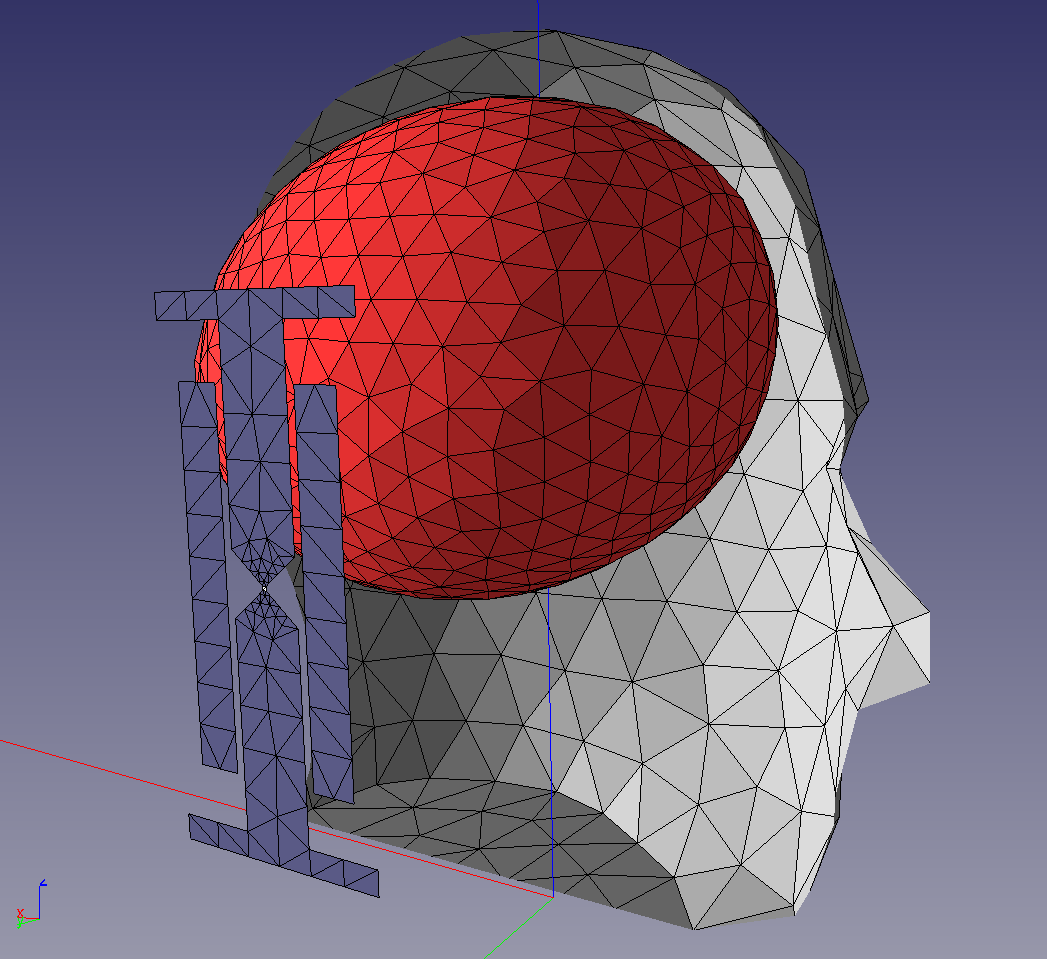
\includegraphics[width=0.9\textwidth]{../img/scene_brain}
\end{figure}
\vskip-1em
\begin{figure}
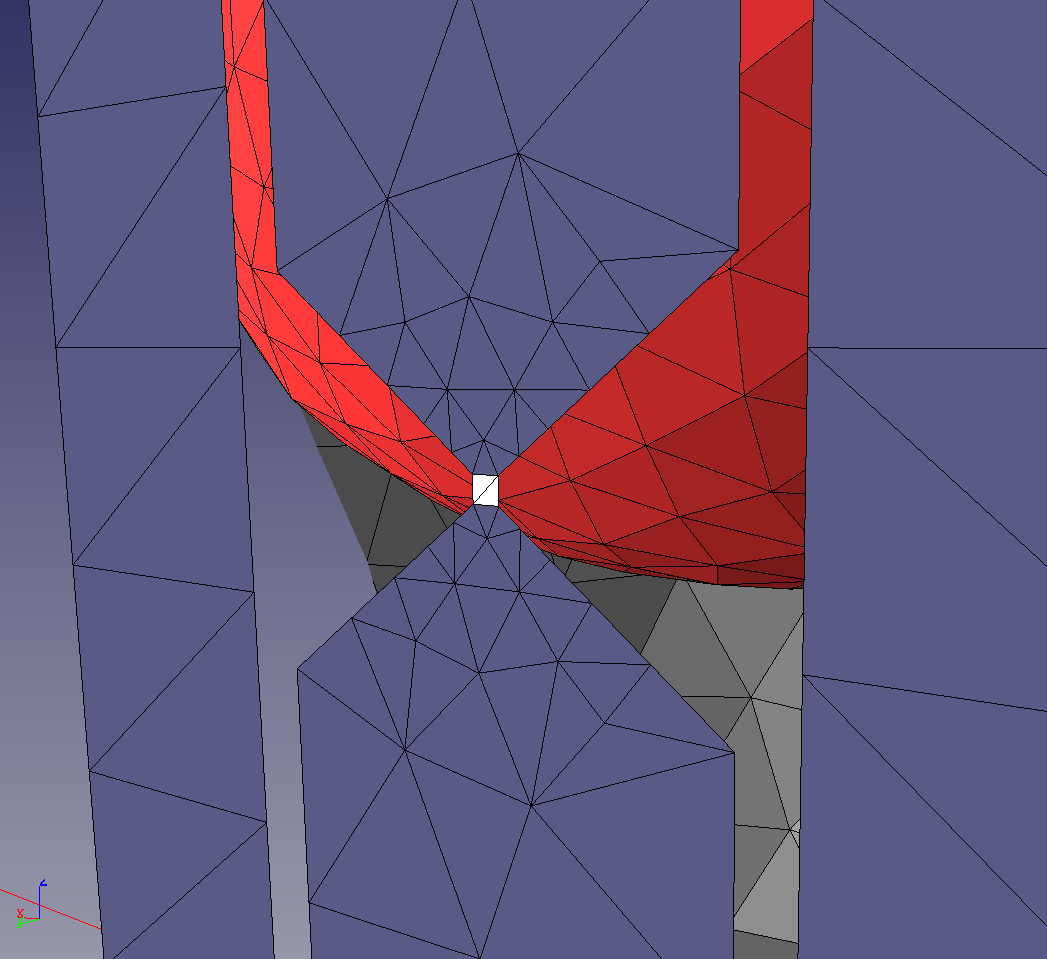
\includegraphics[width=0.9\textwidth,trim={0 200 0 200},clip]{../img/scene_brain_zoom}
\end{figure}
\end{columns}
\vfill
\end{frame}

 % descr
\begin{frame}
\frametitle{Tête simplifiée / Comparaison FD (différences finies)}
\vfill
\begin{columns}
\column{0.6\textwidth}
\scalebox{0.8}{\begin{minipage}{1.25\textwidth}
\begin{figure}
\begin{tabular}{|l|c|c|}
	\hline
	Critère & GD2-RK2 & FD \\ \hline\hline
	Nombre de mailles & 80 k & 90 M \\	\hline
	Nombre d'inconnues & 13 M & 540 M \\	\hline
	Mémoire & 380 Mo & 9 Go \\	\hline
\end{tabular}
\end{figure}
\begin{itemize}
\item Temps physique simulé : 20 ns ;
\item Corrélation empreinte mémoire - coût de calcul ;
\item Résultats cohérents.
\end{itemize}
\end{minipage}}
\column{0.4\textwidth}
\begin{figure}
	\centering
		Position des points.

			\begin{tikzpicture}[scale=3]
			\fill[white] (-0.2,0) rectangle (1.2,1);
			\draw (0,0) rectangle (1,1);
			\fill (0.14,0.45) rectangle (0.16,0.55);
			\draw[thick,fill=gray!20] (0.55,0.5) ellipse (0.25 and 0.35);
			\draw[thick,fill=gray!30] (0.55,0.55) ellipse (0.18 and 0.2);
			\draw (0.15,1) node[below] {SRC};
			\draw (0.55,1) node[below] {TETE};
			\draw[arrows={-latex}] (0.95,0.05) -- (0.95,0.15) node[above] {$\x_1$};
			\draw[arrows={-latex}] (0.95,0.05) -- (0.85,0.05) node[left] {$\x_2$};
			\fill[red] (0.23,0.5) circle (0.015) node[above,red]{$O_1$};
			\fill[red] (0.55,0.5) circle (0.015) node[above,red]{$O_2$};
			\fill[red] (0.94,0.5) circle (0.015) node[above,red]{$O_3$};
			\end{tikzpicture}
\end{figure}
\end{columns}
\begin{columns}
\column{0.33\textwidth}
\begin{figure}
	\centering
		Au point $O_1$.

			\begin{tikzpicture}[scale=0.5]
			\begin{axis}[
			axis lines=middle,
			xlabel=$t$ (ns), x label style={at={(axis cs:11.5,0)},anchor=south},
			ylabel=$\E$ (V/m), y label style={at={(axis cs:0,6)},anchor=west},
			xmin=0,xmax=13,%ymin=-0.1,ymax=1.1,
			xtick={0,2,...,12},%ytick={0,0.5,1},
			%x post scale=1.8,
			%y post scale=1.2,
			%legend style={at={(axis cs:0.9,0.2)},anchor=south west}
			]
			
			\addplot+[
			%thick,
			mark=none,
			color=red,
			] table
			[y expr=-\thisrowno{1}]
			{../tete_elposd/temsi_ez_O1.plt};
			\addlegendentry{FD}
			
			\addplot+[
			%thick,
			mark=none,
			color=blue,
			densely dashed,
			] table
			{../tete_elposd/teta_ez_O1.plt};
			\addlegendentry{GD}
			
			\end{axis}
			\end{tikzpicture}
\end{figure}
\column{0.33\textwidth}
\begin{figure}
	\centering
		Au point $O_2$.

			\begin{tikzpicture}[scale=0.5]
			\begin{axis}[
			axis lines=middle,
			xlabel=$t$ (ns), x label style={at={(axis cs:11.5,0)},anchor=south},
			ylabel=$\E$ (V/m), y label style={at={(axis cs:0,0.175)},anchor=west},
			xmin=0,xmax=13,%ymin=-0.1,ymax=1.1,
			xtick={0,2,...,12},%ytick={0,0.5,1},
			%x post scale=1.8,
			%y post scale=1.2,
			%legend style={at={(axis cs:0.9,0.2)},anchor=south west}
			]
			
			\addplot+[
			%thick,
			mark=none,
			color=red,
			] table
			[y expr=-\thisrowno{1}]
			{../tete_elposd/temsi_ez_O2.plt};
			\addlegendentry{FD}
			
			\addplot+[
			%thick,
			mark=none,
			color=blue,
			densely dashed,
			] table
			{../tete_elposd/teta_ez_O2.plt};
			\addlegendentry{GD}
			
			\end{axis}
			\end{tikzpicture}
\end{figure}
\column{0.33\textwidth}
\begin{figure}
	\centering
		Au point $O_3$.

			\begin{tikzpicture}[scale=0.5]
			\begin{axis}[
			axis lines=middle,
			xlabel=$t$ (ns), x label style={at={(axis cs:11.5,0)},anchor=south},
			ylabel=$\E$ (mV/m), y label style={at={(axis cs:0,70)},anchor=west},
			xmin=0,xmax=13,%ymin=-0.1,ymax=1.1,
			xtick={0,2,...,12},%ytick={0,0.5,1},
			%x post scale=1.8,
			%y post scale=1.2,
			%legend style={at={(axis cs:0.9,0.2)},anchor=south west}
			]
			
			\addplot+[
			%thick,
			mark=none,
			color=red,
			] table
			[y expr=-\thisrowno{1}*1000]
			{../tete_elposd/temsi_ez_O3.plt};
			\addlegendentry{FD}
			
			\addplot+[
			%thick,
			mark=none,
			color=blue,
			densely dashed,
			] table
			[y expr=\thisrowno{1}*1000]
			{../tete_elposd/teta_ez_O3.plt};
			\addlegendentry{GD}
			
			\end{axis}
			\end{tikzpicture}
\end{figure}
\end{columns}
\vfill
\end{frame}

 % comp fd
\begin{frame}
\frametitle{Tête simplifiée / Performances}
\vfill
%\scalebox{0.9}{\begin{minipage}{1.11\textwidth}
Temps de calcul pour un pas de temps optimal :
\begin{figure}
\centering
\begin{tabular}{|l|c|c|c|}
	\hline
	Méthode & Temps de calcul (h) & Accélérateur & Accélération \\ \hline\hline
	FD & 2.24 & CPU & 0.53 \\	\hline\hline
	GD2-RK2 & 1.19 & GPU & 1 \\	\hline
	GD2-LRK2 & 1.71 & GPU & 0.70* \\	\hline
	GD2-LTS2 & 0.84 & GPU & 1.42* \\	\hline\hline
	GD1-RK2 & 0.31 & GPU & 3.84 \\	\hline
	GD1-LTS2 & 0.18 & GPU & 6.61* \\	\hline
\end{tabular}
\vfill
* : Le pas de temps optimal RK2 est 2 fois plus grand que le plus petit pas de temps LRK2/LTS2.
\end{figure}
\vfill
\begin{itemize}
\item []
\begin{itemize}
\item [CPU] : Intel Dual Xeon E5-2650 v4 (48 c.)
\item [GPU] : NVidia GeForce GTX 1080 Ti
\end{itemize}
\end{itemize}
\vfill
\end{frame}

 % resultats

\subsection{Corps humain complet}

\begin{frame}
\frametitle{Corps humain / Description}
\begin{columns}
\column{0.55\textwidth}
\scalebox{0.8}{\begin{minipage}{1.25\textwidth}
\begin{itemize}
\item 12 organes dont le squelette ;
\item $5\,840\,122$ tétraèdres découpés ;
\item Permittivités relatives : Gabriel, 1996 ;
\item Condition limite absorbante (PML de Bérenger) ;
\item Antenne Bluetooth rayonnant à 2.45 GHz ;
\item Facteur d'échelle d'ordre 1300 ;
\item Forme d'onde (6 ns) : Gaussienne modulée.
\end{itemize}
\end{minipage}}
\vskip-1em
\begin{columns}
\column{0.5\textwidth}
\scalebox{0.7}{\begin{minipage}{1.42\textwidth}
\begin{figure}
	\centering
		\begin{tabular}{|c|c|c|c|c|}
			\hline
			Matériau & $\EPrm_r$\\ \hline\hline
			cerveau & $48.34$ \\	\hline
			cœur & $58.67$ \\	\hline
			poumon & $22$ \\	\hline
			foie & $41.82$ \\	\hline
			bile & $60$ \\	\hline
			rate & $56.75$ \\	\hline
			pancréas & $56.75$ \\	\hline
			rein & $56.83$ \\	\hline
			colon & $48.5$ \\	\hline
			vessie & $20$ \\	\hline
			muscle & $50$ \\	\hline
			os & $11.41$ \\	\hline
			cartilage & $36$ \\	\hline
			vide & $1$ \\	\hline
		\end{tabular}
\end{figure}
\end{minipage}}
\column{0.5\textwidth}
\begin{figure}
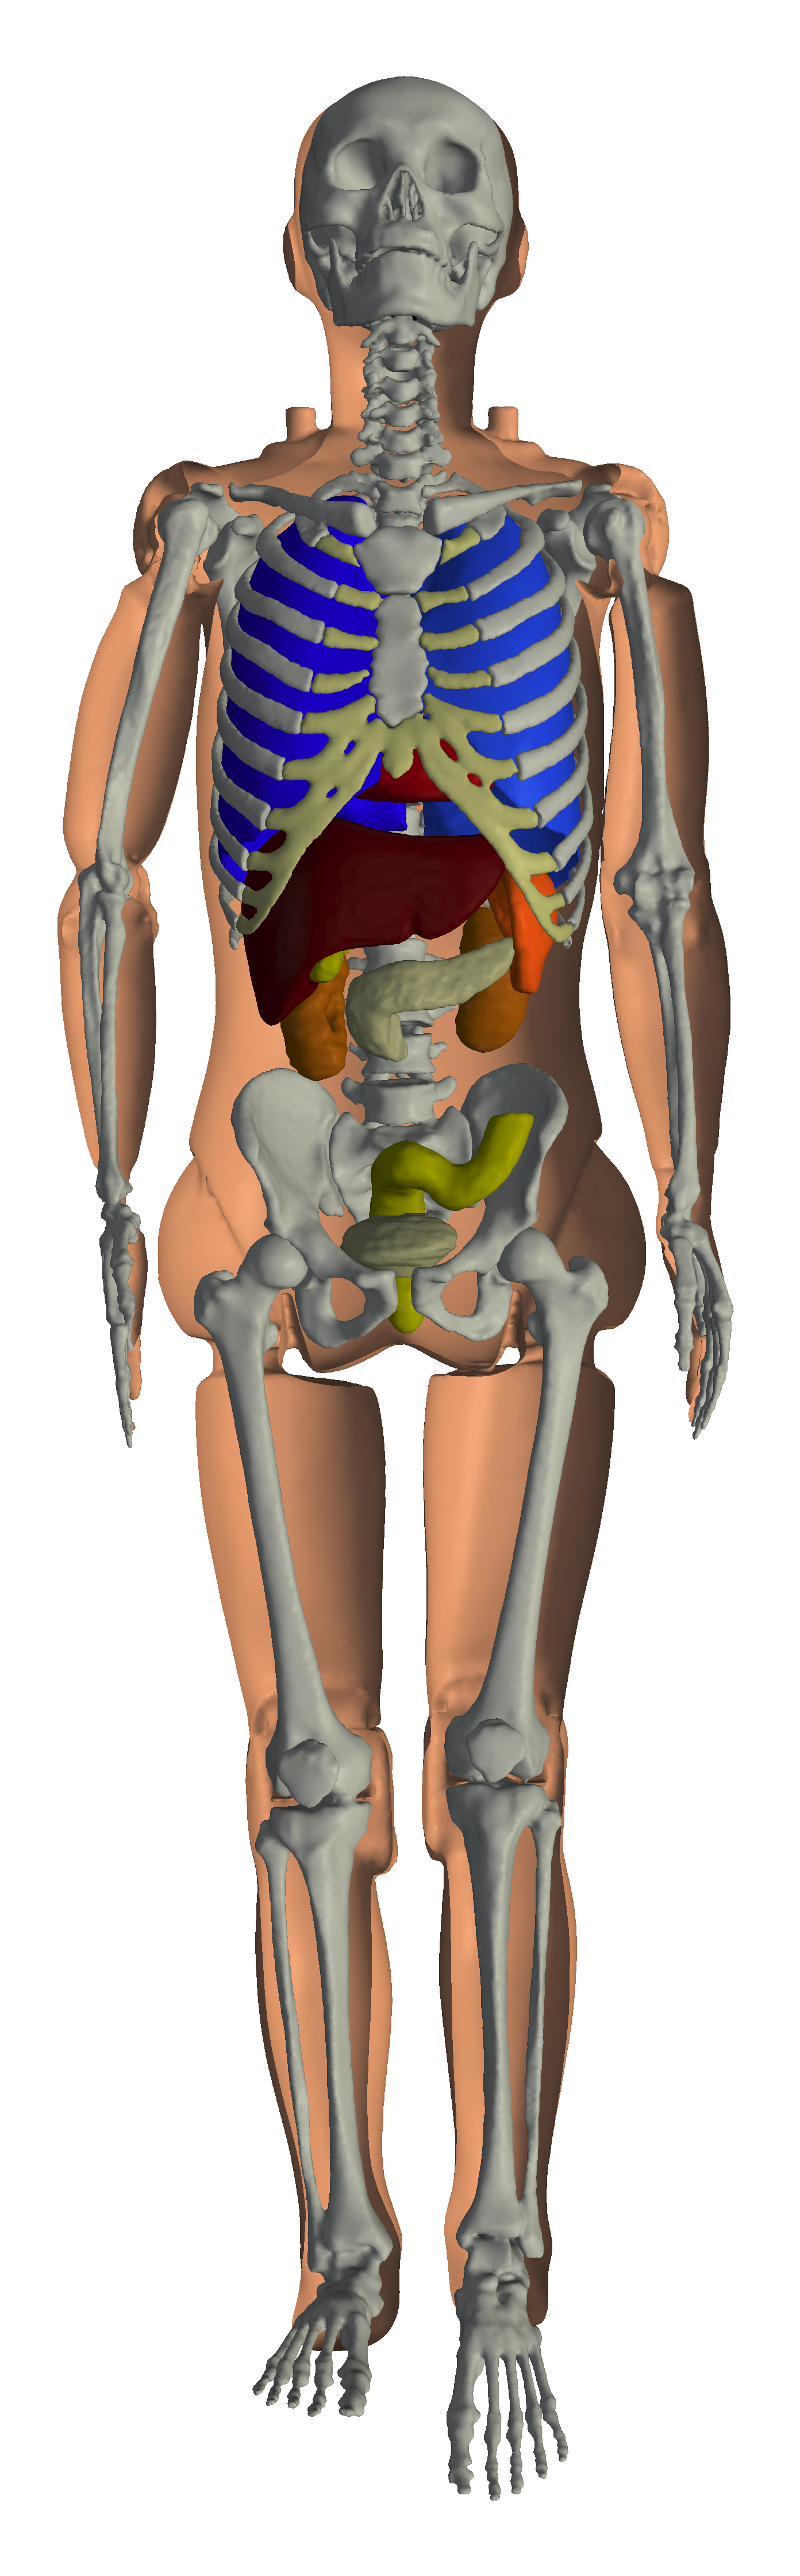
\includegraphics[width=0.5\textwidth]{../img/kyoto}
\end{figure}
\end{columns}
\column{0.45\textwidth}
\vskip-1em
\begin{figure}
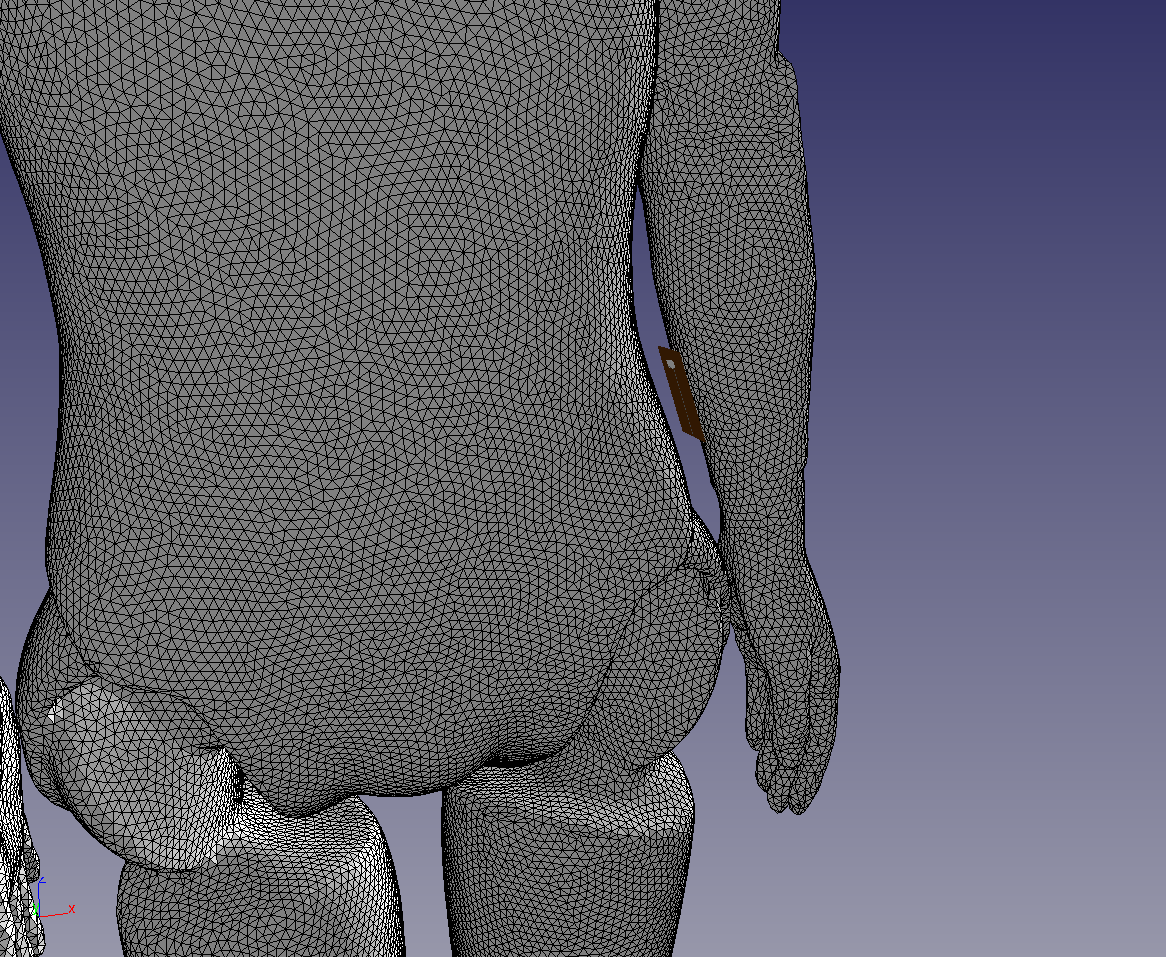
\includegraphics[width=0.8\textwidth]{../img/wide_ltcc}
\end{figure}
\vskip-1em
\begin{figure}
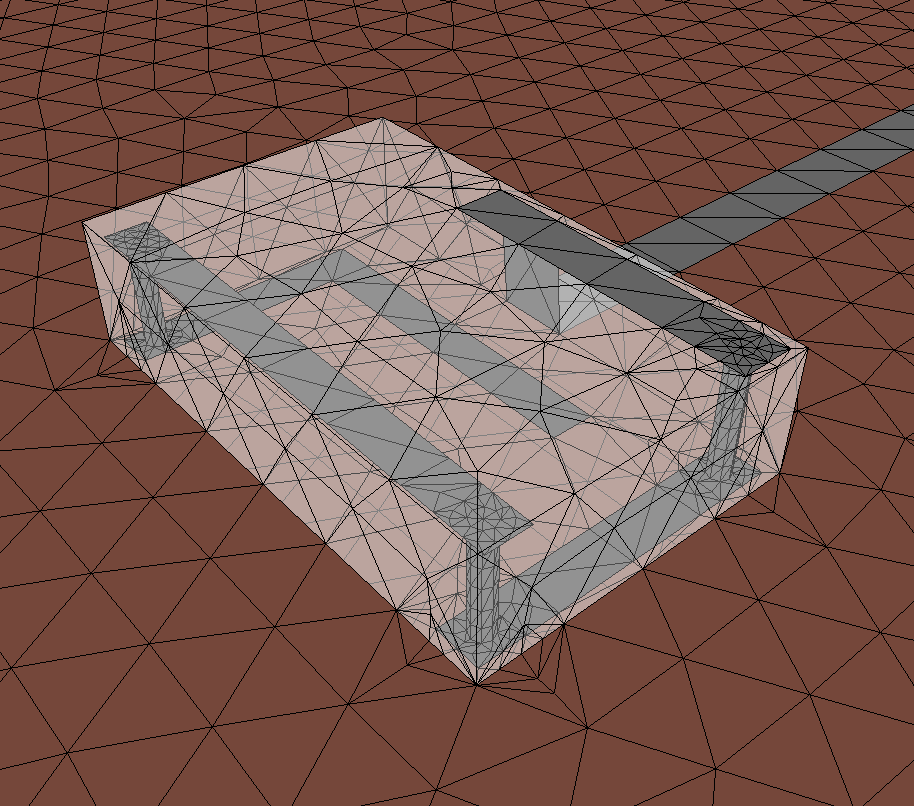
\includegraphics[width=0.8\textwidth,
%trim={0 200 0 200},clip
]{../img/ltcc}
\end{figure}
\end{columns}
\vfill
\end{frame}

 % descr
\begin{frame}
\frametitle{Corps humain / Résultats}
\vfill
\begin{columns}
\column{0.6\textwidth}
%\scalebox{0.9}{\begin{minipage}{1.11\textwidth}
\begin{figure}
\begin{tabular}{|l|c|c|}
	\hline
	Critère & GD1-RK2 & GD2-RK2 \\ \hline\hline
	Nombre de mailles & 23.4 M & 23.4 M \\	\hline
	Nombre d'inconnues & 1123 M & 3791 M \\	\hline
	Mémoire & 40 Go & 100 Go \\	\hline
\end{tabular}
\end{figure}
\vfill
\begin{itemize}
\item Temps physique simulé : 10 ns ;
\item Machine AxesSim :\\ 8 GPU NVidia GeForce GTX 1080 Ti 11 Go ;
\item Temps machine GD1-RK2 : 2072 heures ;
\item Temps humain GD1-RK2 : 10.79 jours.
\end{itemize}
%\end{minipage}}
\vfill
\begin{figure}
\centering
\href{run:../img/modE_xoz_ogv.mp4}{\textcolor{blue}{VIDEO plan (xOz)}}

1 s de vidéo $\leftrightarrow$ 6.5 h de calcul intensif

1 s de vidéo $\leftrightarrow$ 0.25 ns physiques
\end{figure}
\column{0.4\textwidth}
\begin{figure}
\centering
(xOz), $t = 3$ ns.

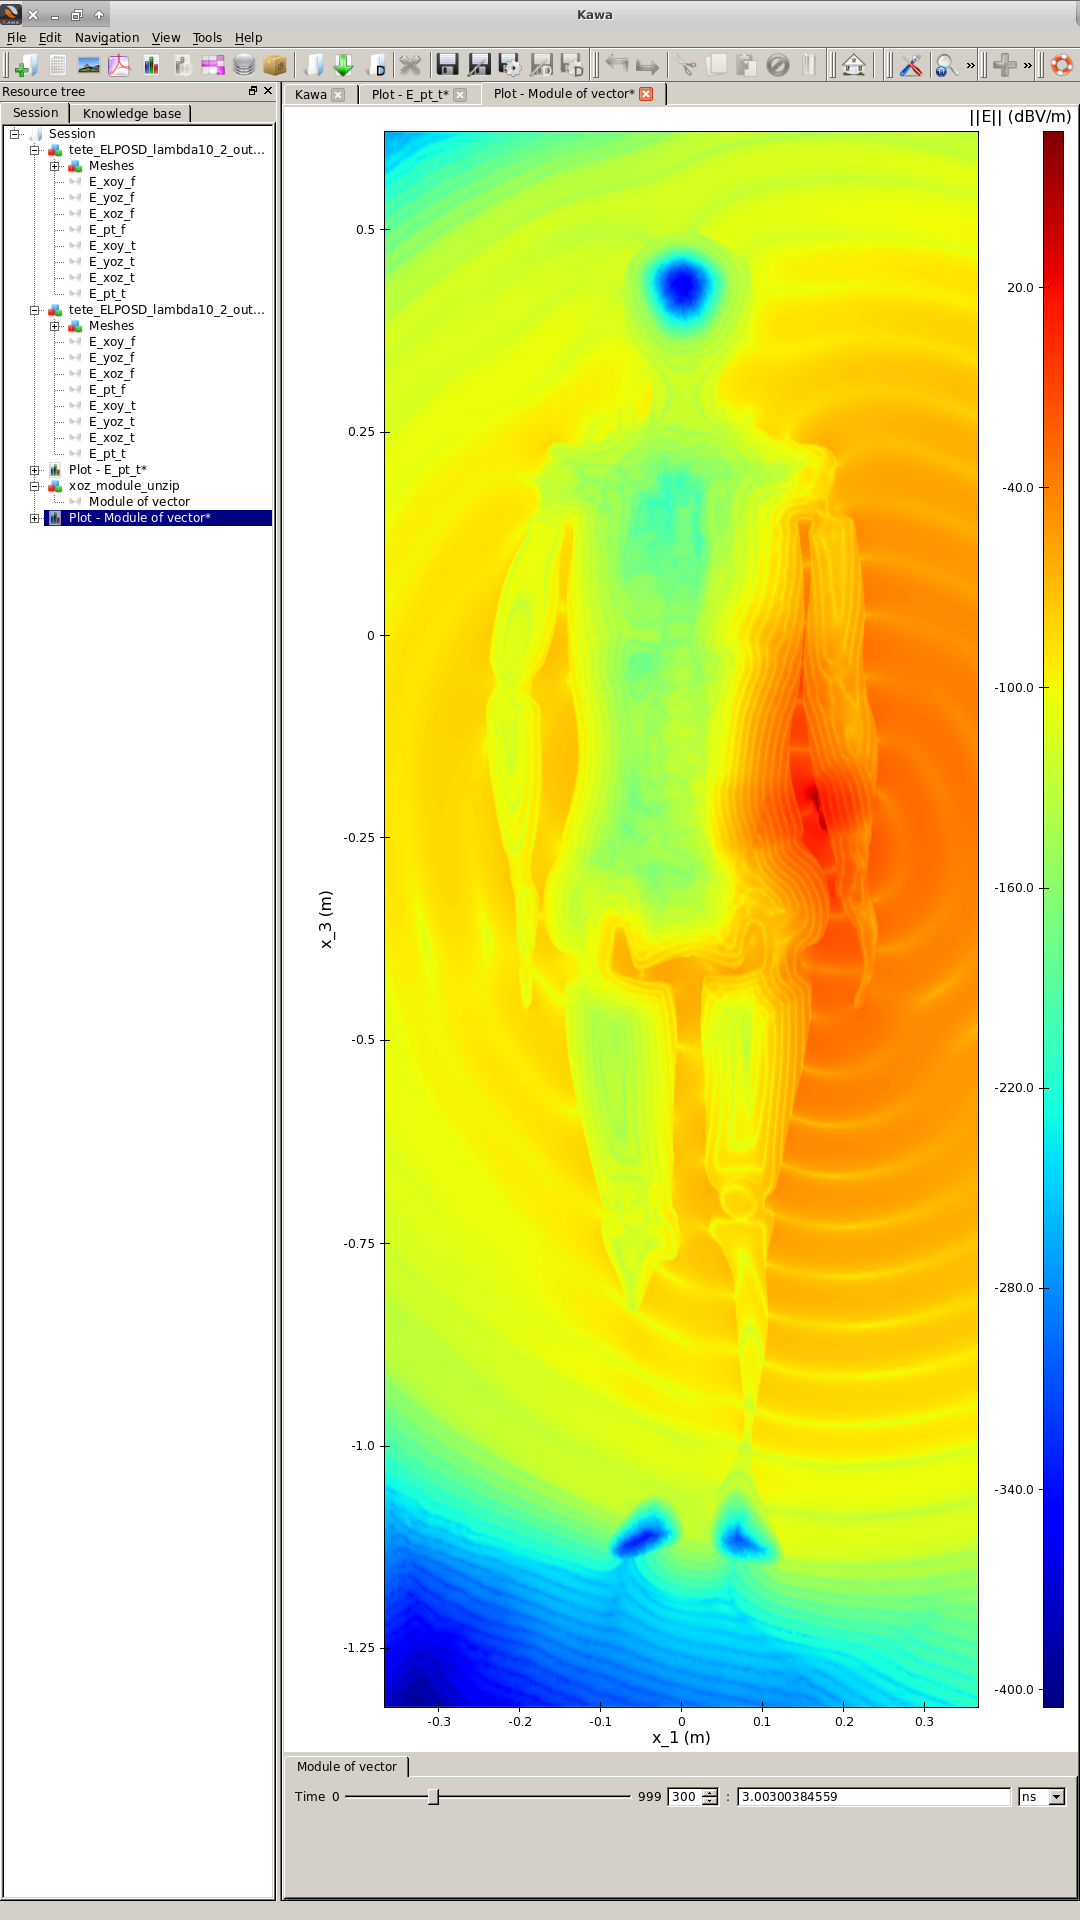
\includegraphics[
	width=0.66\linewidth,
	trim={317 170 8 108},clip
	]{../img/kyoto_3ns}
\end{figure}
\end{columns}
\vfill
\end{frame}

 % resultat simu
\begin{frame}
\frametitle{Corps humain / Efficacité MPI}
\vfill
\begin{itemize}
\item Scalabilités faible et forte évaluées sur le Mésocentre de Strasbourg :
\begin{itemize}
\item [=>] Très efficace (perte $< 10$ \%) à partir de 500 k mailles (1.3 Go) par nœud MPI ;
\end{itemize}
\vfill
\item Scalabilité forte évaluée sur PizDaint sur le corps humain jusqu'à 256 GPU :
\begin{itemize}
\item 2000 heures de calcul obtenues par PRACE ;
\item $3^{\mathrm{eme}}$ machine au TOP500 jusqu'en juin 2018 ($5^{\mathrm{eme}}$ depuis) ;
\item Plus de 5000 GPU NVidia Tesla P100 (équivalent GTX 1080 Ti) ;
\end{itemize}
\end{itemize}
\vfill
\scalebox{0.8}{\begin{minipage}{1.25\textwidth}
\begin{figure}
	\centering
Efficacités constatées :

		\begin{tabular}{|c|c|c|c|}
			\hline
			$\#$GPU & GD1-RK2 & GD2-RK2 & GD3-RK2 \\ \hline\hline
			$4$ & 1* & - & - \\	\hline
			$8$ & $0.980$ & 1* & - \\	\hline
			$16$ & $0.955$ & $0.980$ & 1* \\	\hline
			$32$ & $0.909$ & $0.943$ & $0.970$ \\	\hline
			$64$ & $0.844$ & $0.889$ & $0.919$ \\	\hline
			$128$ & $0.749$ & - & - \\	\hline
			$256$ & $0.612$ & - & - \\	\hline
		\end{tabular}

		* : Simulation prise comme référence pour l'ordre courant.
\end{figure}
\end{minipage}}
\begin{itemize}
\item [=>] Temps de calcul GD1-RK2 sur 256 GPU pour 10 ns estimé à :
\begin{align*}
2072 / 256 / 0.612 = 13.23 \ \mathrm{heures.}
\end{align*}
\end{itemize}
\vfill
\end{frame}

 % scala MPI


\section{Conclusion}






\begin{frame}
\frametitle{Conclusion}
\vfill
Points abordés :
\begin{itemize}
\item Description du solveur GD Teta-CLAC qui permet de résoudre efficacement les équations de Maxwell en se conformant aux contraintes géométriques ;
\item Présentation d'une partie des améliorations apportées dans le cadre de cette thèse CIFRE qui ont permis de faire passer une simulation \textit{réaliste} sur un modèle de corps humain présentant un haut niveau de détail ;
\item Preuve donnée de la possibilité de traiter ce type de problématique en un temps humain très raisonnable ;
\item C'est l'amélioration constante du solveur GD Teta-CLAC qui a permis d'obtenir ces résultats encore hypothétiques il y a $3$ ans.
\end{itemize}
\vfill
La suite :
\begin{itemize}
\item Simulation sur corps humain à l'aide du schéma à pas de temps local ;
\item Utilisation de maillages hybrides (hexaèdres, tétraèdres) afin de réduire les contraintes induites par le découpage des tétraèdres tout en bénéficiant des simplifications apportées par les hexaèdres ;
\item Consolider l'exécution hybride CPU/GPU pour plus de polyvalence au niveau des accélérateurs et tirer profit de toute la puissance de calcul disponible.
\end{itemize}
\end{frame}



%TODO ccl et perspectives



\begin{frame}

\includegraphics[width=\textwidth]{../img/fin}

\vfill
 
\huge{\centerline{Merci pour votre attention.}}
\end{frame}


\end{document}
